% Appendices

%========================================
% APPENDIX 1: ADDITIONAL MATERIAL
%========================================
\chapter{Listings}
\label{listings}

\begin{lstlisting}[language=Python, caption=Preprocessing Function for EfficientNet and ResNet, label=PreprocessingFunction]
def preprocess_dataset(src_root, dest_root, size=(224, 224)):
	
	if not os.path.exists(dest_root):
		os.makedirs(dest_root, exist_ok=True)
	
	for category in os.listdir(src_root):
		src_path = os.path.join(src_root, category)
		dest_path = os.path.join(dest_root, category)
		
		if not os.path.isdir(src_path):
			continue
		
		if not os.path.exists(dest_path):
			os.makedirs(dest_path, exist_ok=True)
		
		print(f"Category: {category}")
		
		for img_name in tqdm(os.listdir(src_path)):
			img_path = os.path.join(src_path, img_name)
			save_path = os.path.join(dest_path, img_name)
			
			try:
				img = cv2.imread(img_path)
				if img is None: continue
				
				gray = cv2.cvtColor(img, cv2.COLOR_BGR2GRAY)
				faces = face_cascade.detectMultiScale(gray, 1.1, 4)
				
				if len(faces) > 0:
					faces = sorted(faces, key=lambda f: f[2] * f[3], reverse=True)
					x, y, w, h = faces[0]
					face_img = img[y:y+h, x:x+w]
				else:
					face_img = img
				
				face_img = cv2.resize(face_img, size)
				
				cv2.imwrite(save_path, face_img)
			except Exception as e:
				print(f"Error {img_name}: {e}")
\end{lstlisting}
\pagebreak

\begin{lstlisting}[language=Python, caption=Calculation of weights for the CrossEntropyLoss, label=weights]
class_counts = torch.tensor([3995, 4097, 7215, 4965, 4830, 3171], dtype=torch.float)
total_samples = class_counts.sum()

weights = total_samples / (len(class_counts) * class_counts)
weights = weights.to(device)

criterion = nn.CrossEntropyLoss(weight=weights)
\end{lstlisting}

\begin{lstlisting}[language=Python, caption=Backbone-freeze and Hyperparameters for EfficientNet, label=efficientNetModel]
efficientnet_b0_model = models.efficientnet_b0(pretrained=True)

for param in efficientnet_b0_model.parameters():
	param.requires_grad = False

num_features = efficientnet_b0_model.classifier[1].in_features
efficientnet_b0_model.classifier = nn.Sequential(
	nn.Dropout(p=0.5, inplace=True),
	nn.Linear(num_features, 6)
)

optimizer_efficientnet = torch.optim.Adam(efficientnet_b0_model.parameters(), lr=0.001, weight_decay=1e-4)
scheduler_efficientnet = torch.optim.lr_scheduler.ReduceLROnPlateau(optimizer_efficientnet, 'max', patience=2)
\end{lstlisting}

\chapter{Accuracy and Loss Graphs}
\label{accAndLoss}

\begin{figure}[h]
	\centering
	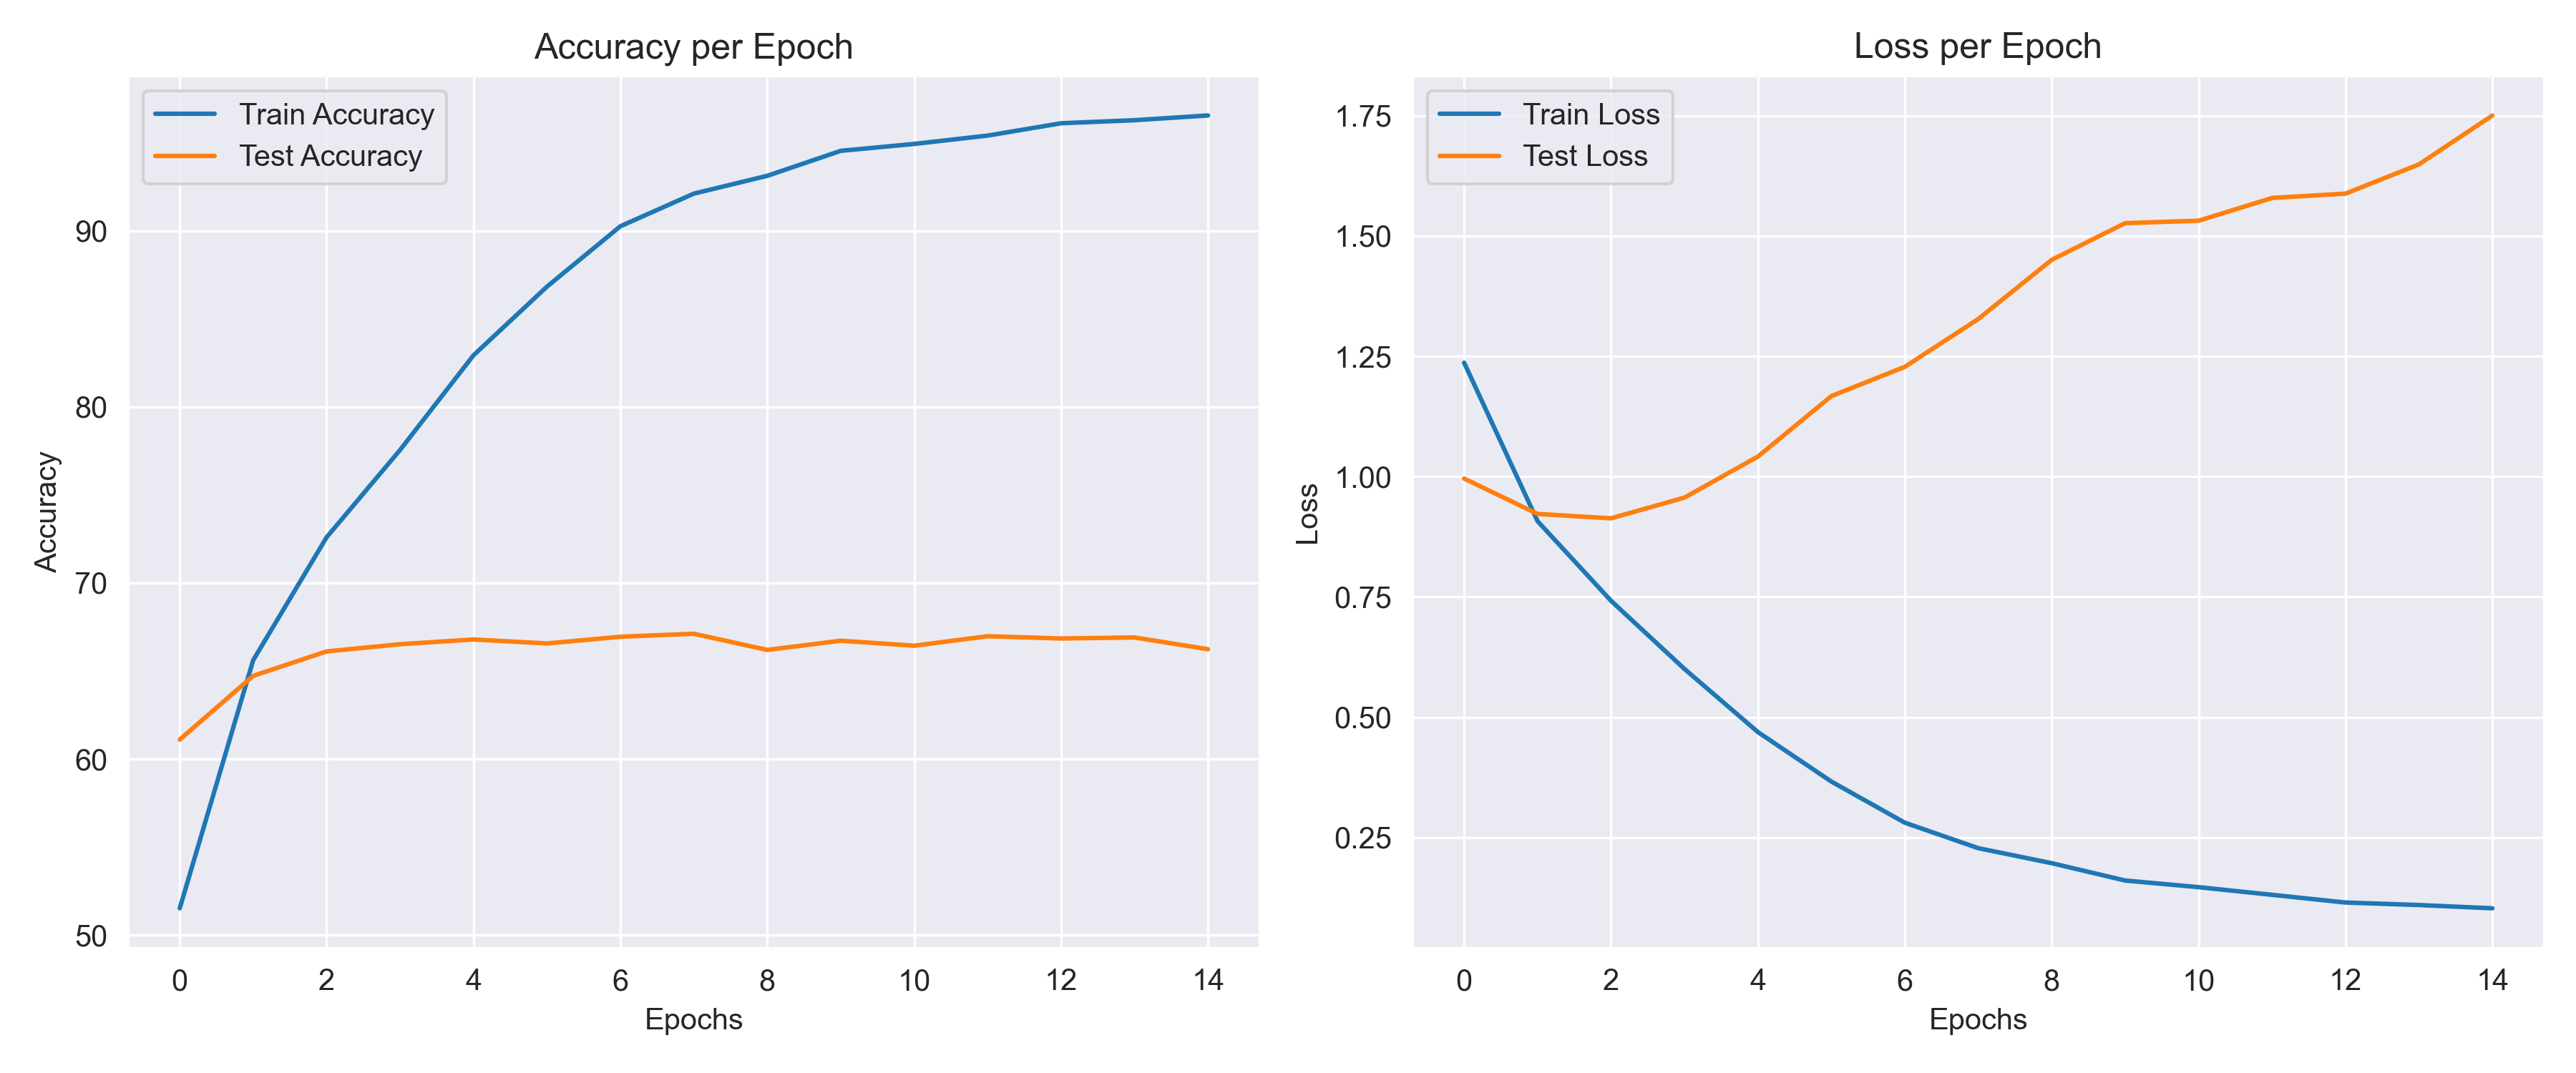
\includegraphics[width=1\textwidth]{figures/acc_loss_efficientnet.png}
	\caption{Accuracy and Loss Graph - EfficientNet-B0 - pre-improvements}
	\label{fig:accLossEfficientnet01}
\end{figure}

\begin{figure}[h]
	\centering
	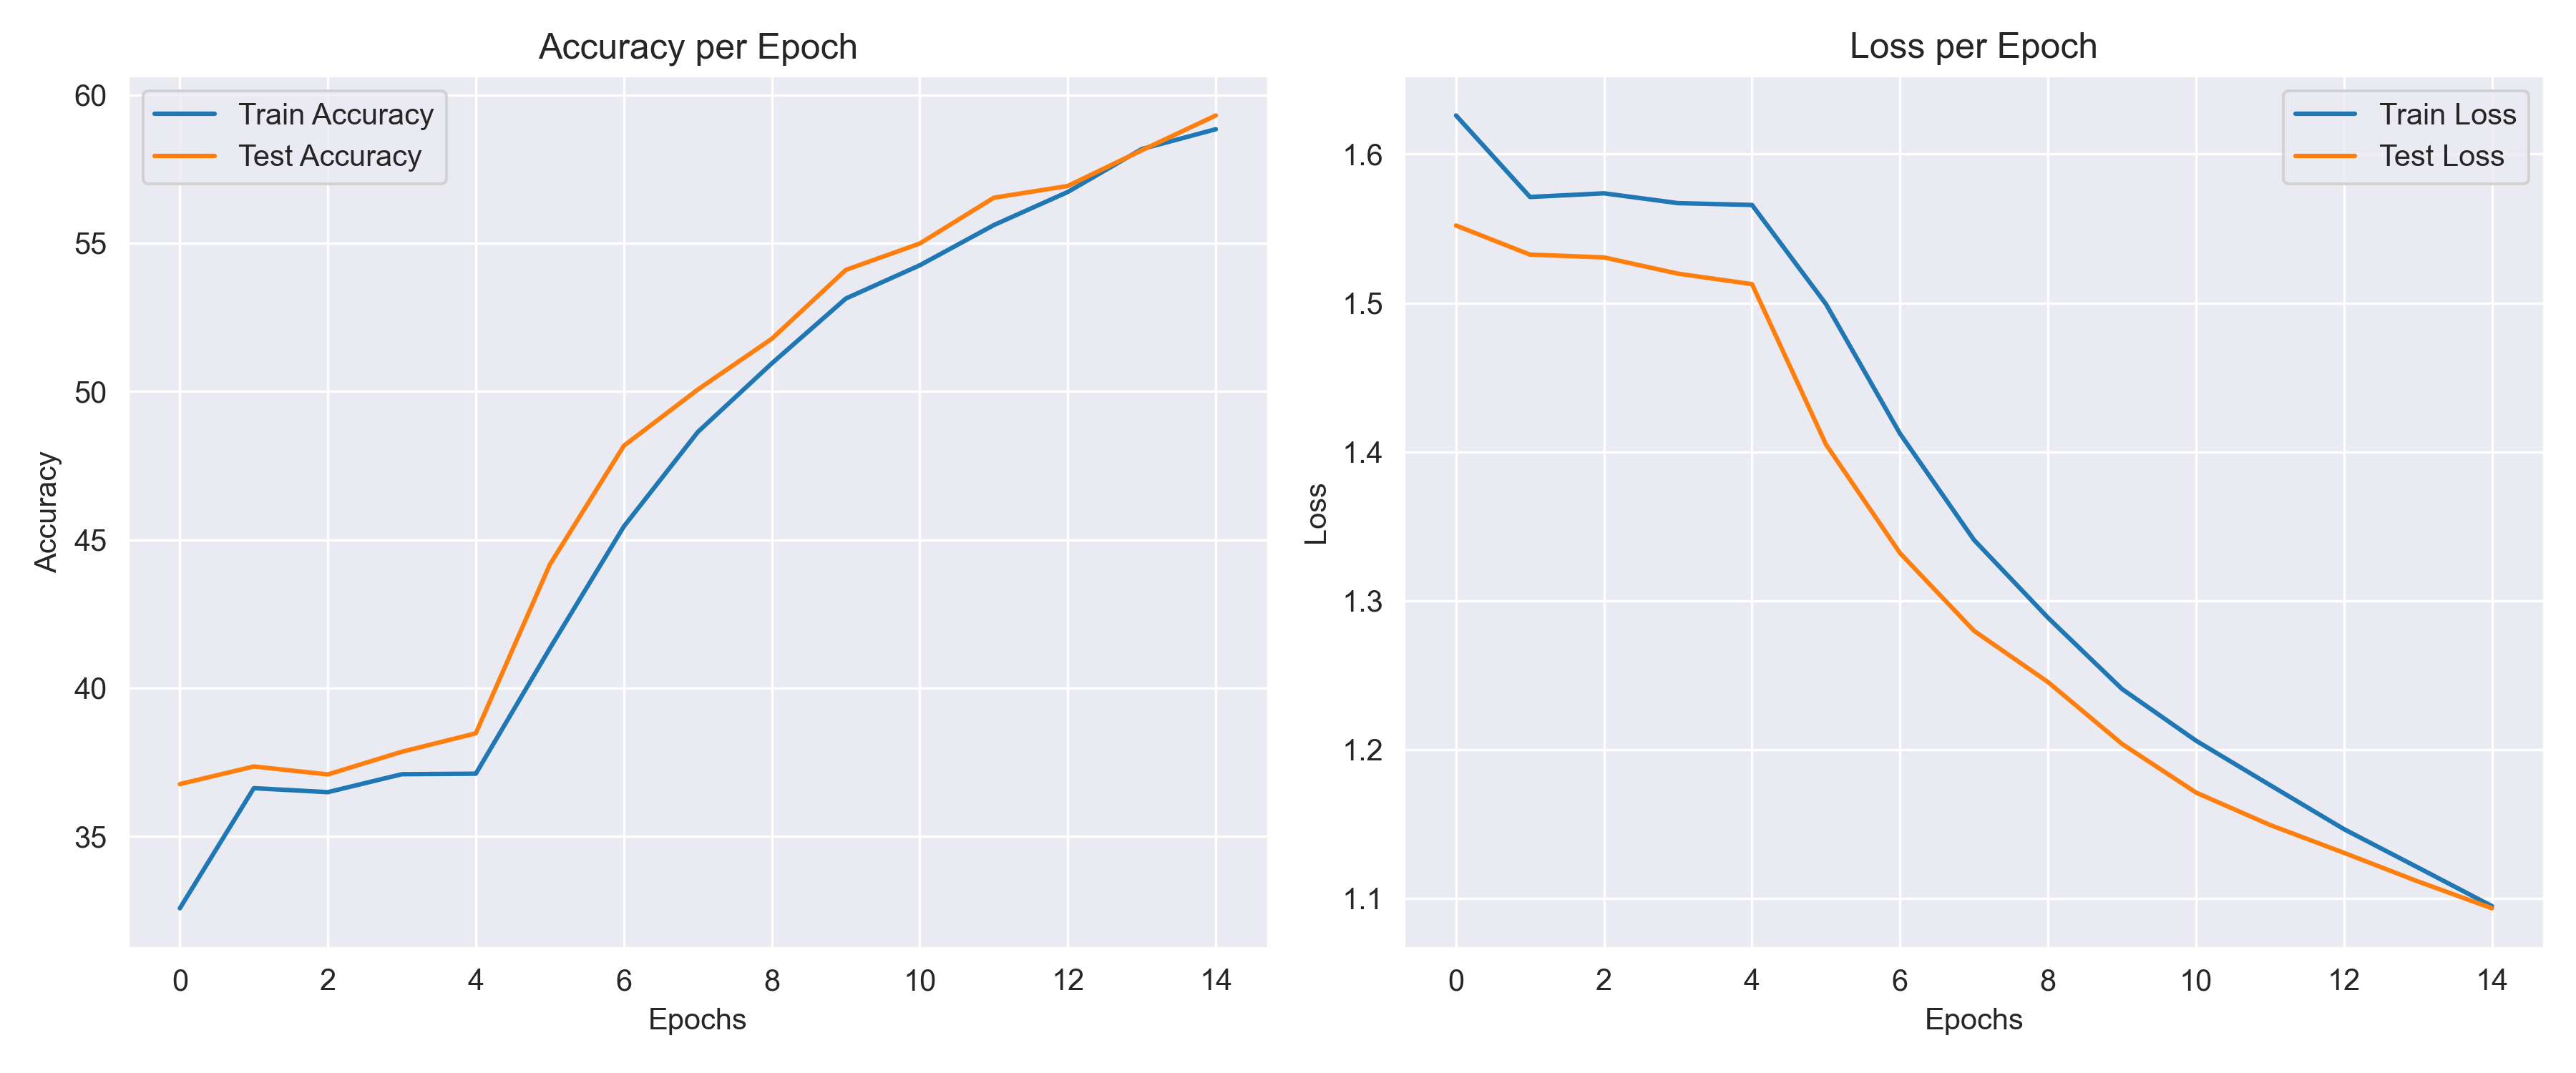
\includegraphics[width=1\textwidth]{figures/acc_loss_efficientnet_02.png}
	\caption{Accuracy and Loss Graph - EfficientNet-B0 - post-improvements}
	\label{fig:accLossEfficientnet02}
\end{figure}

\begin{figure}[h]
	\centering
	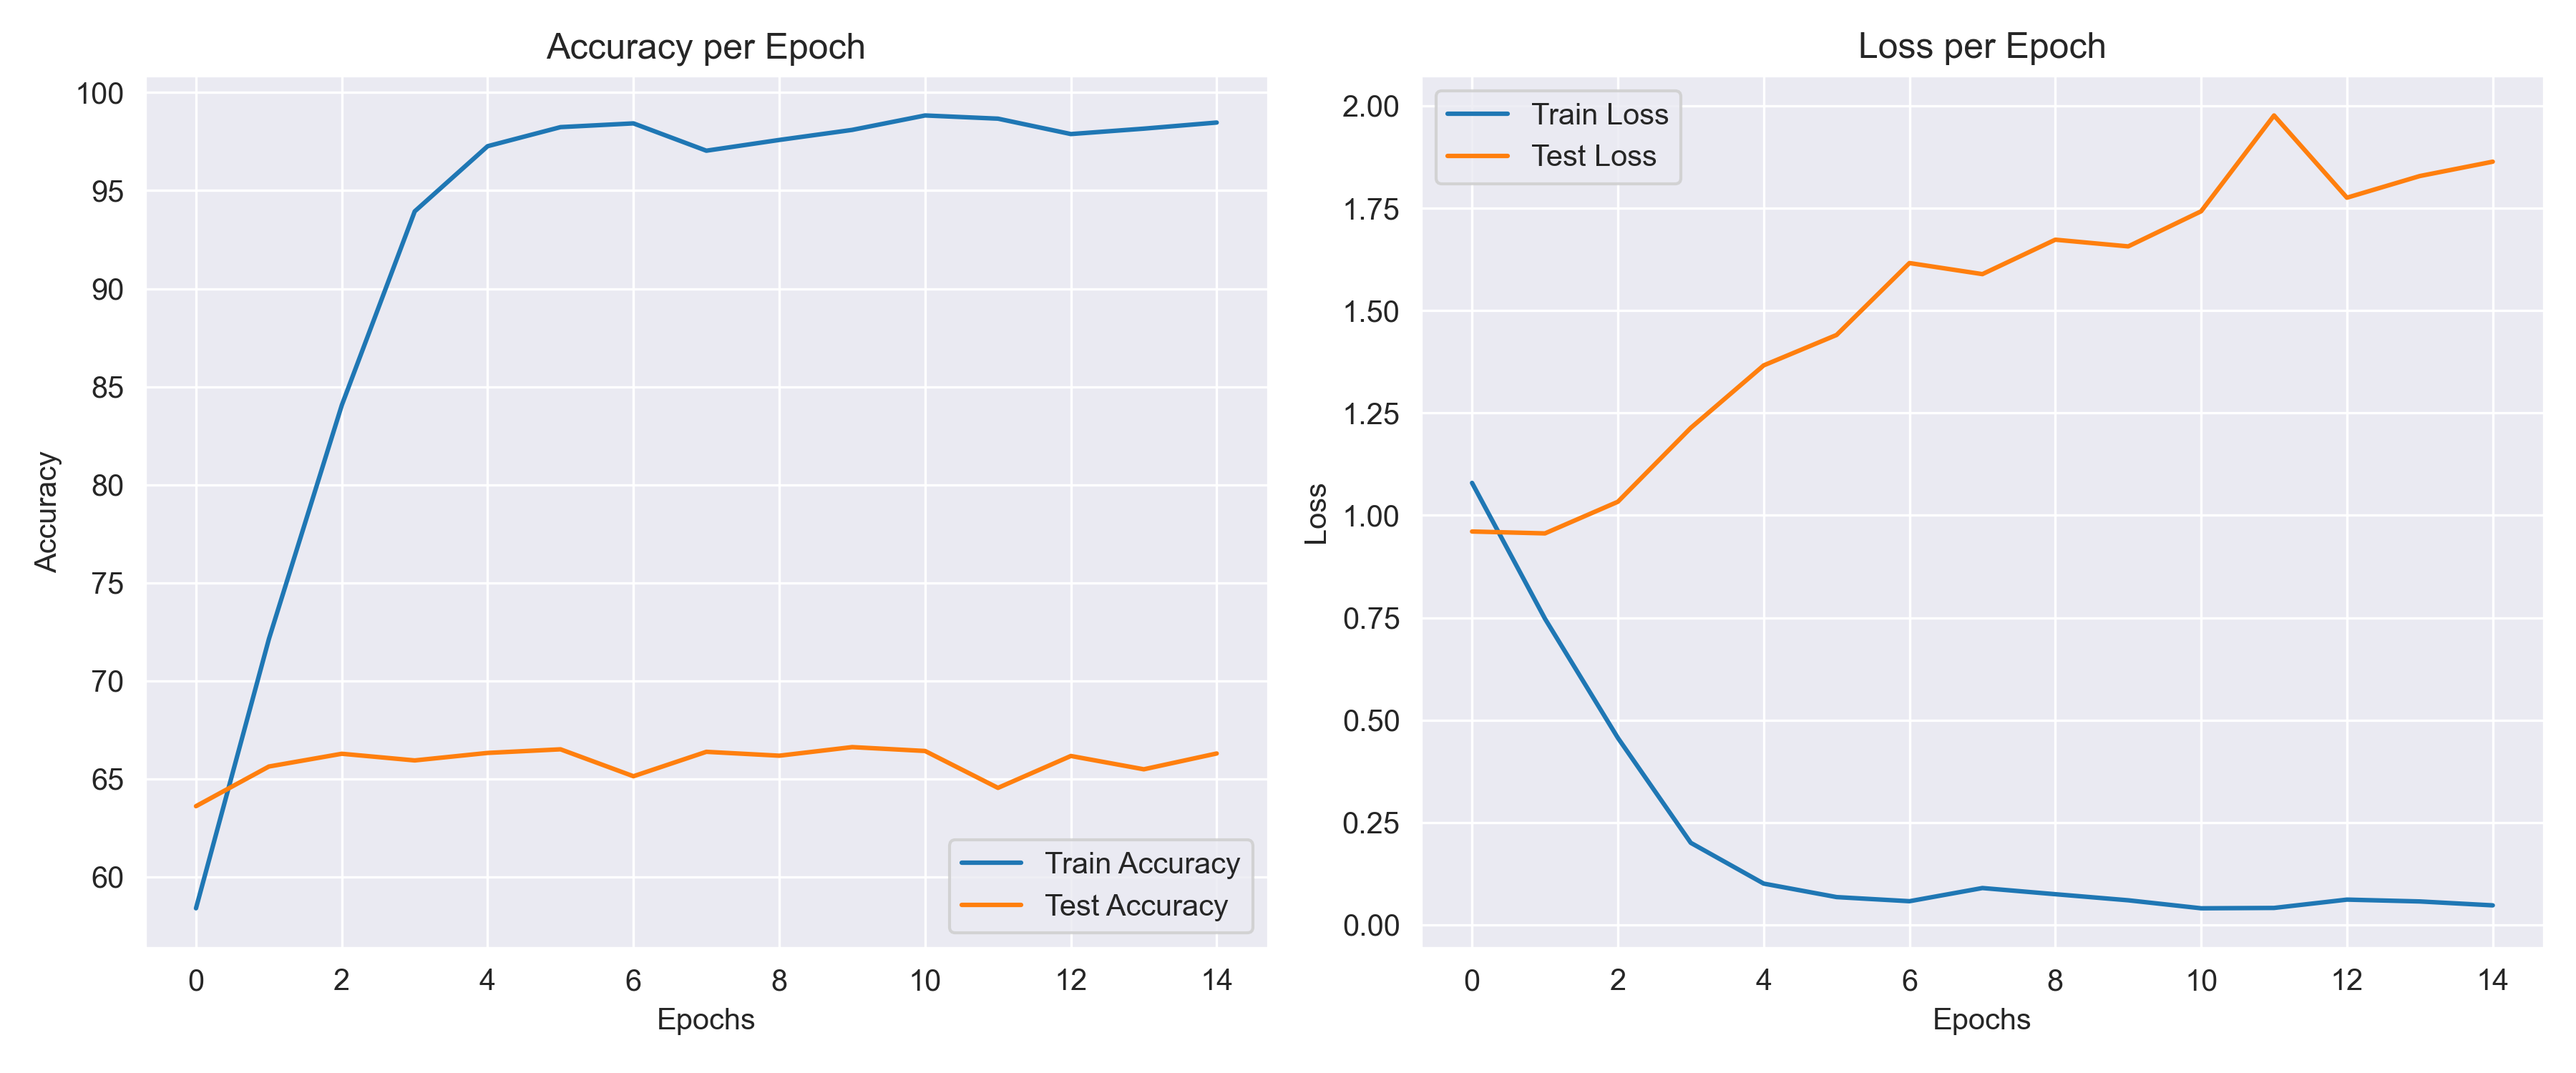
\includegraphics[width=1\textwidth]{figures/acc_loss_resnet.png}
	\caption{Accuracy and Loss Graph - ResNet18 - pre-improvements}
	\label{fig:accLossResNet01}
\end{figure}

\begin{figure}[h]
	\centering
	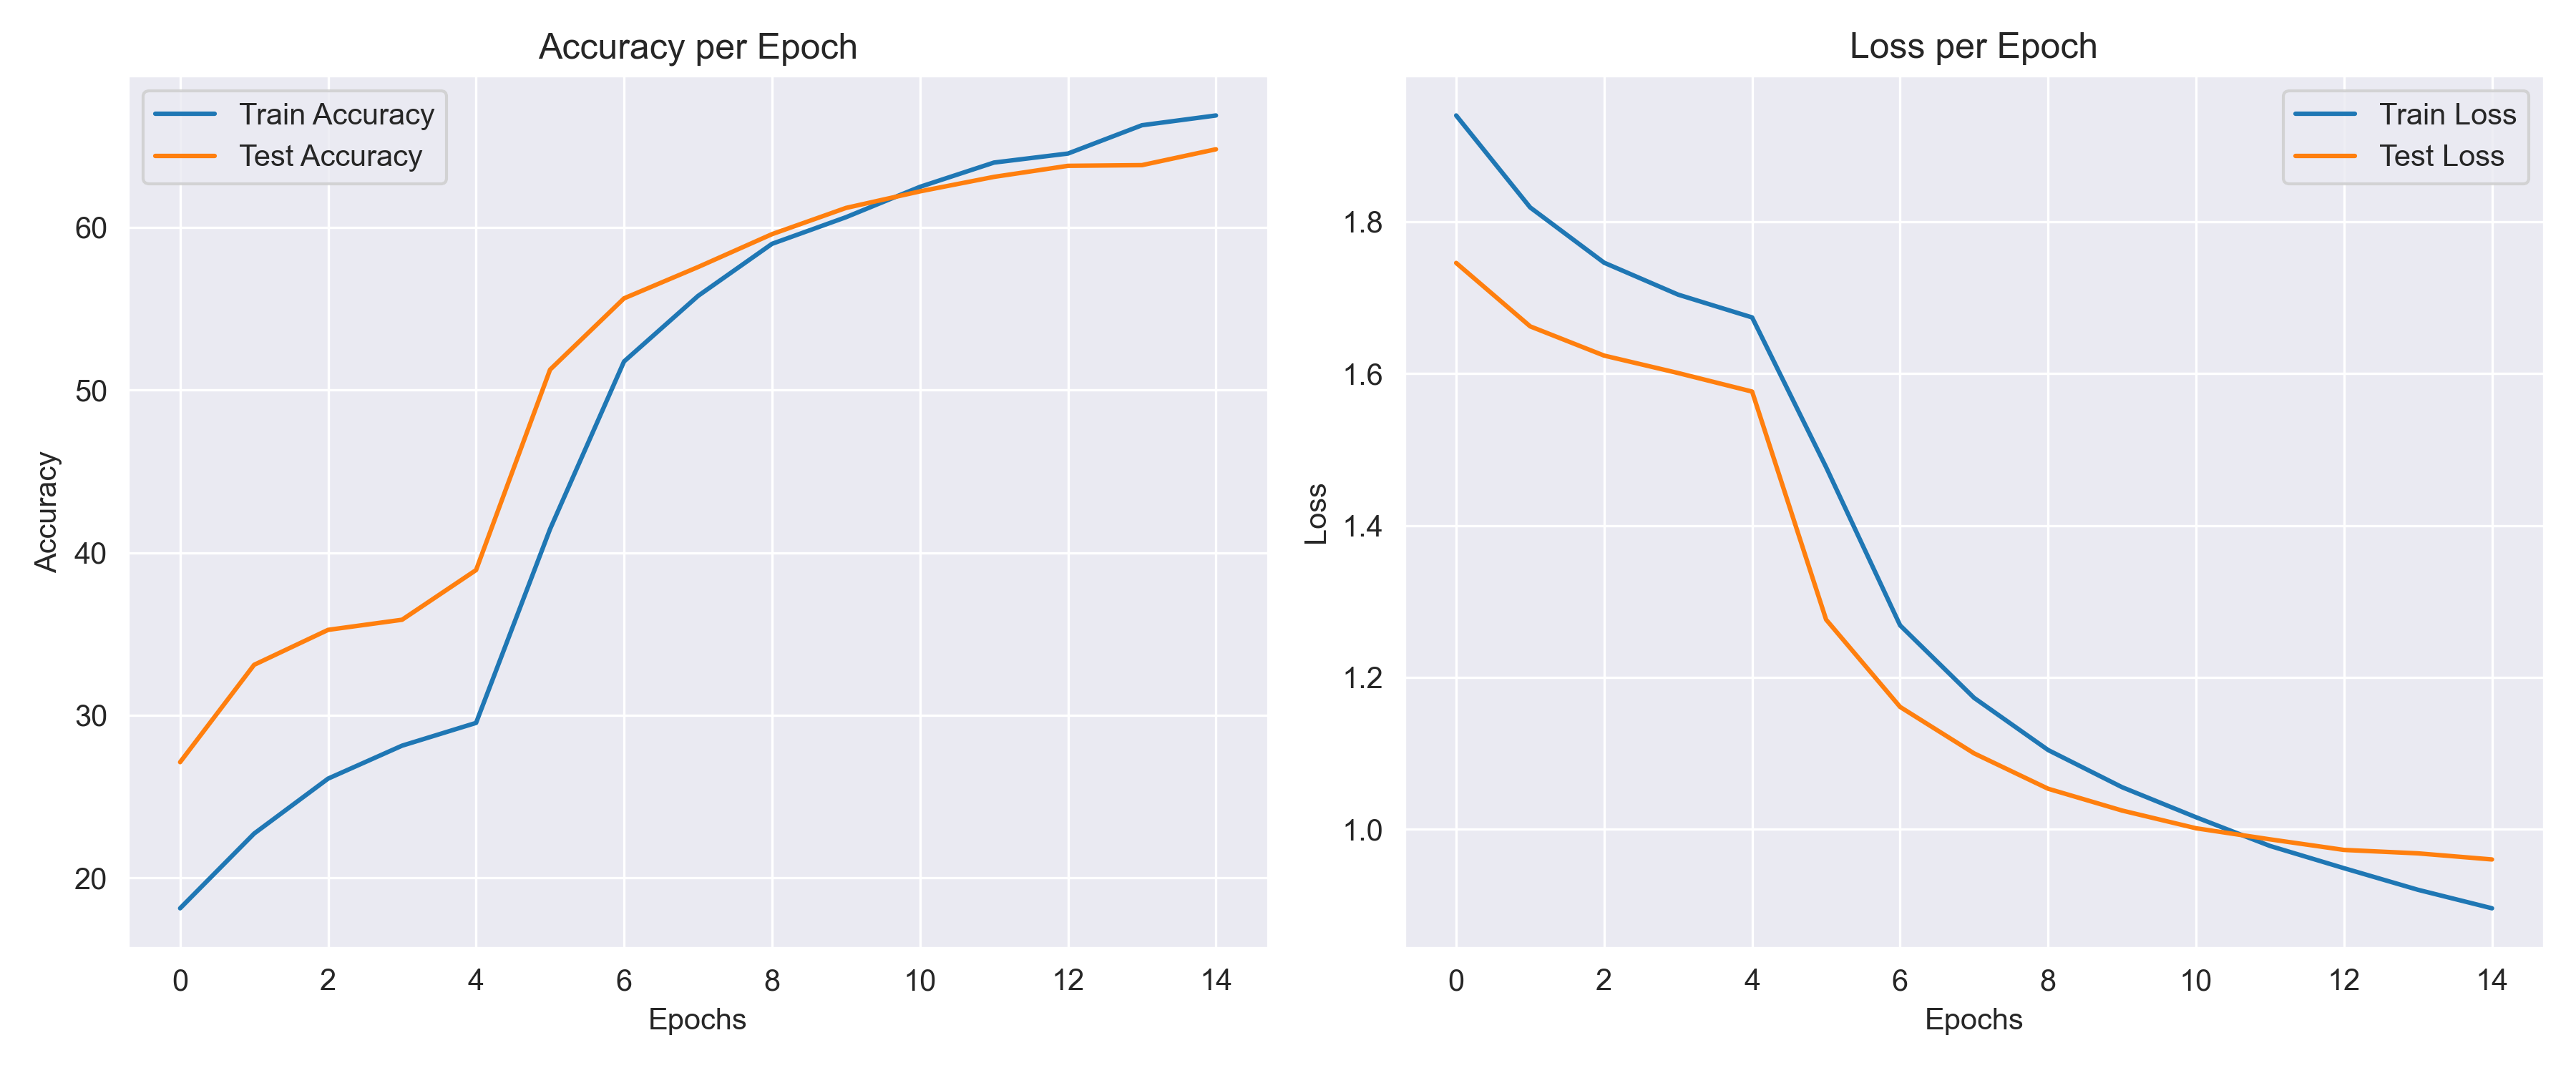
\includegraphics[width=1\textwidth]{figures/acc_loss_resnet_02.png}
	\caption{Accuracy and Loss Graph - ResNet18 - post-improvements}
	\label{fig:accLossResNet02}
\end{figure}

\begin{figure}[h]
	\centering
	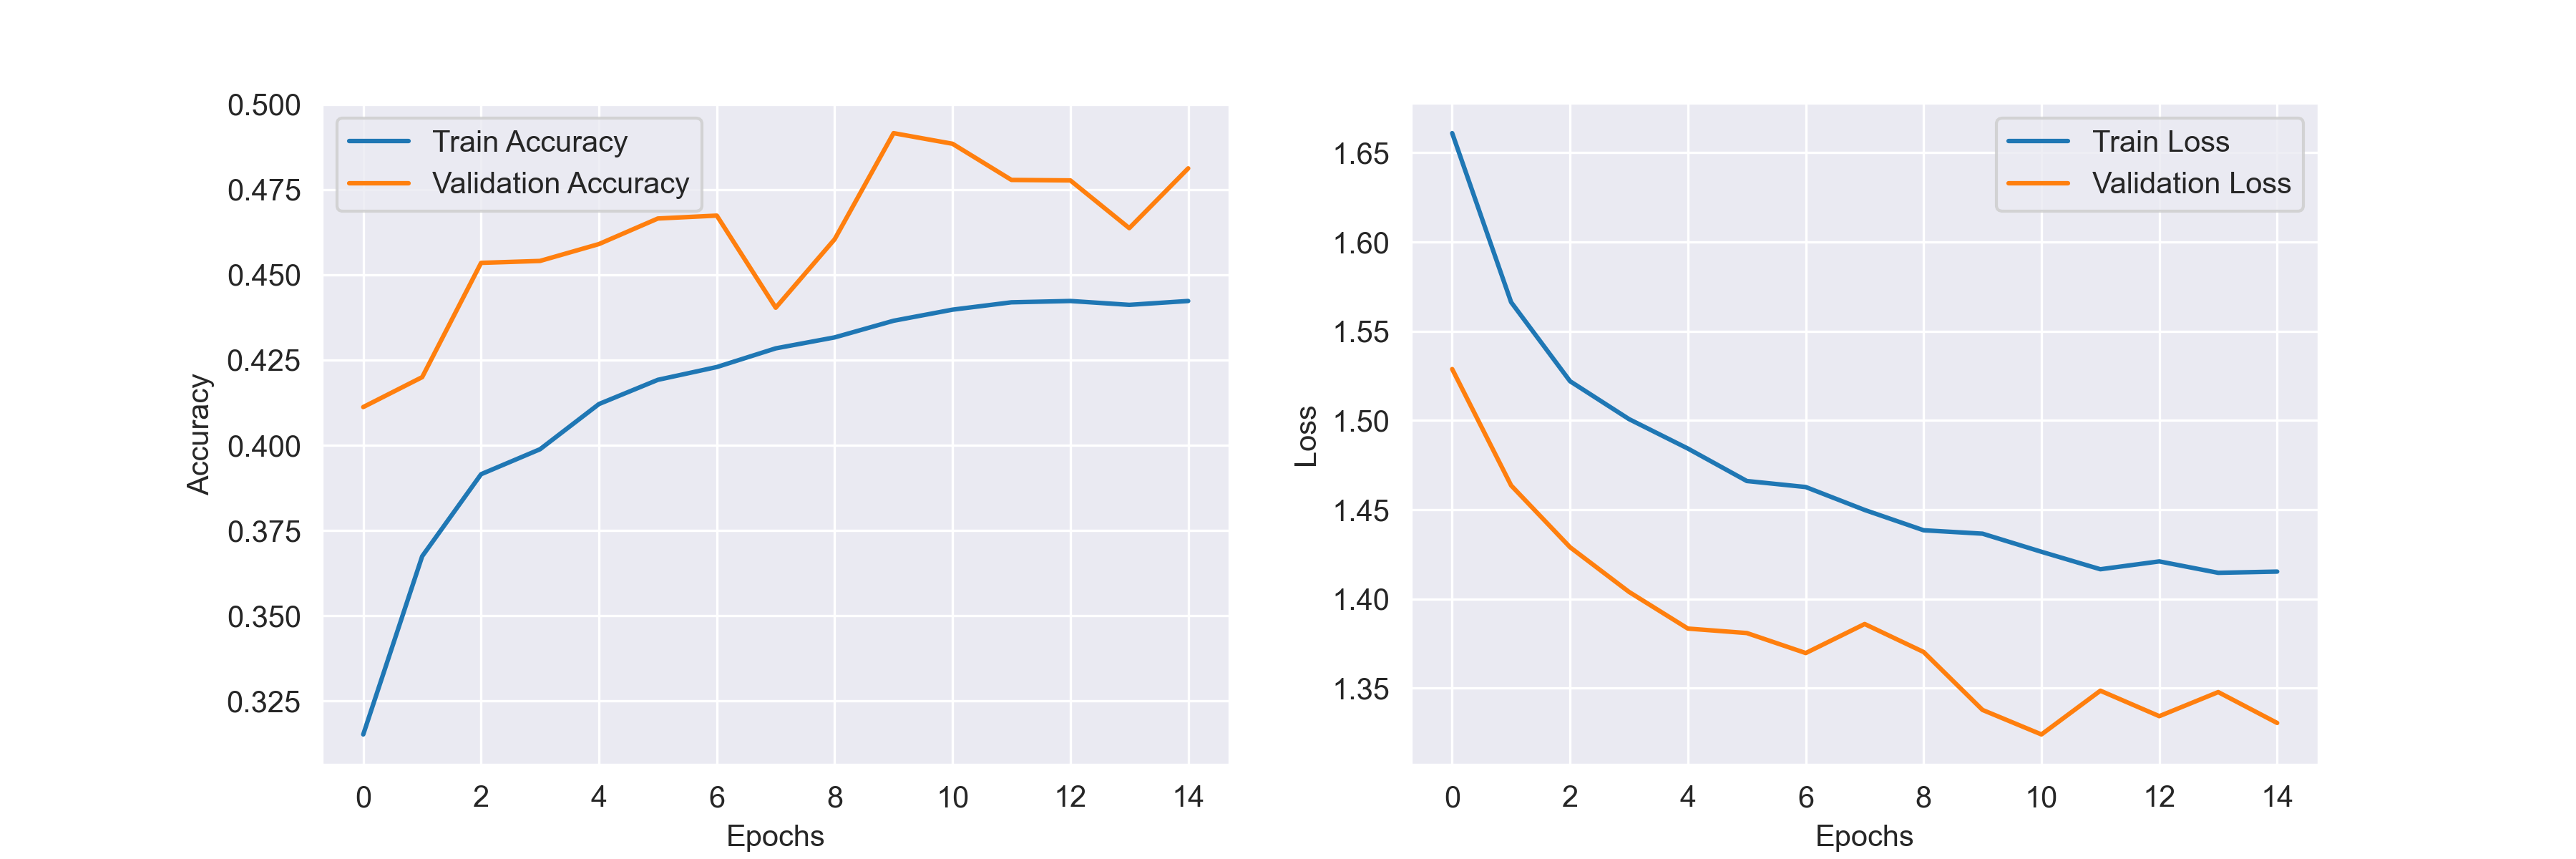
\includegraphics[width=1\textwidth]{figures/acc_loss_vgg16.png}
	\caption{Accuracy and Loss Graph - VGG16}
	\label{fig:accLossVGG16}
\end{figure}

\chapter{Confusion Matrices}
\label{cm}

\begin{figure}[h]
	\centering
	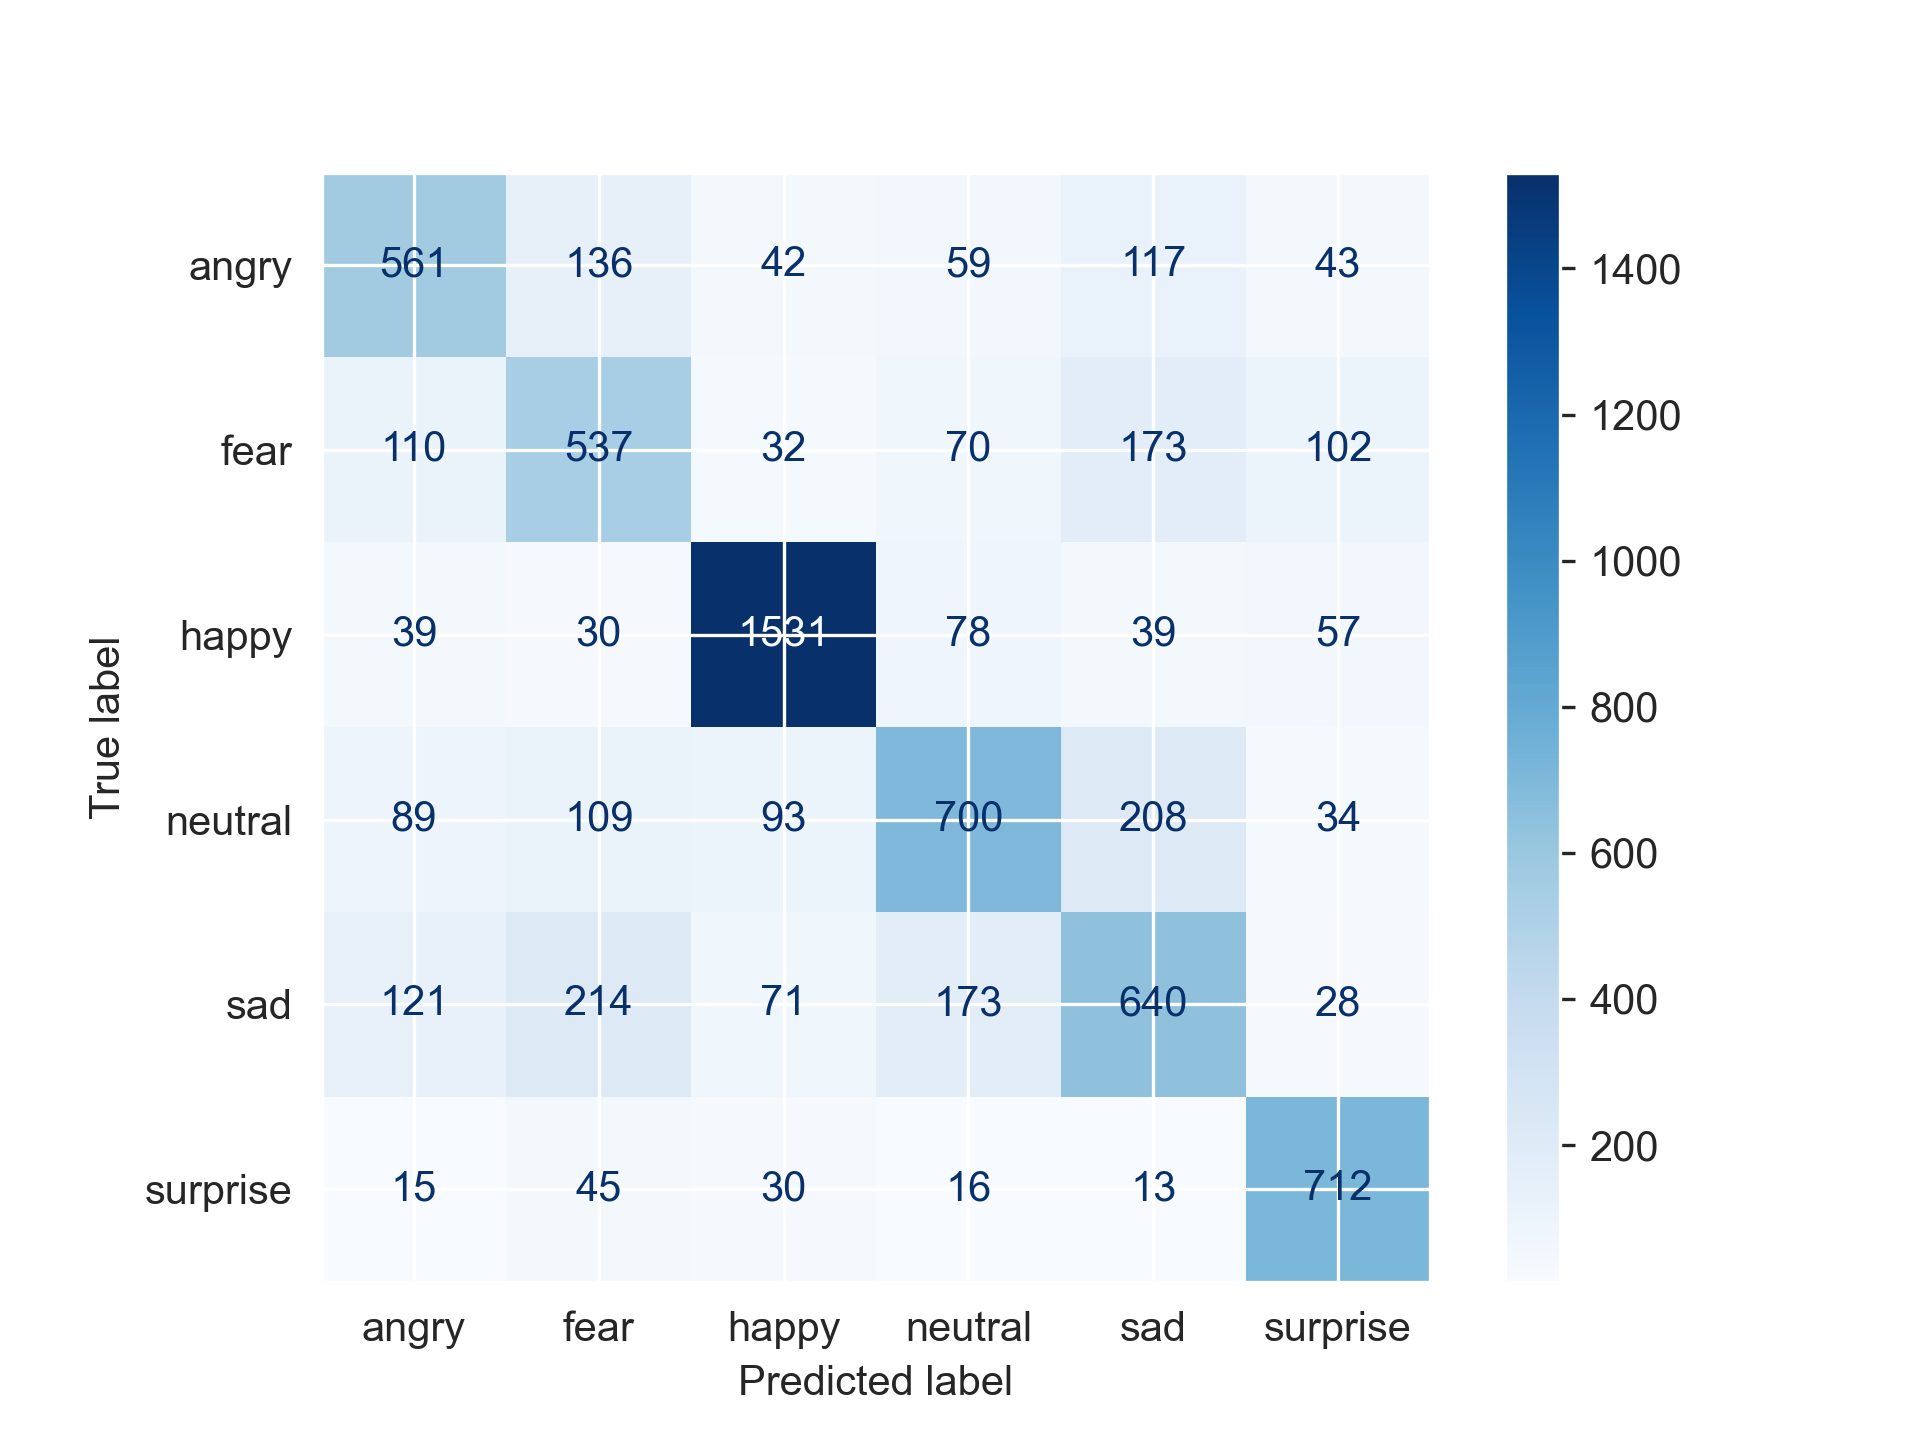
\includegraphics[width=1\textwidth]{figures/cm_efficientnet_b0_trained.png}
	\caption{Confusion Matrix - EfficientNet-B0 - pre-improvements}
	\label{fig:cm_efficientnet_01}
\end{figure}

\begin{figure}[h]
	\centering
	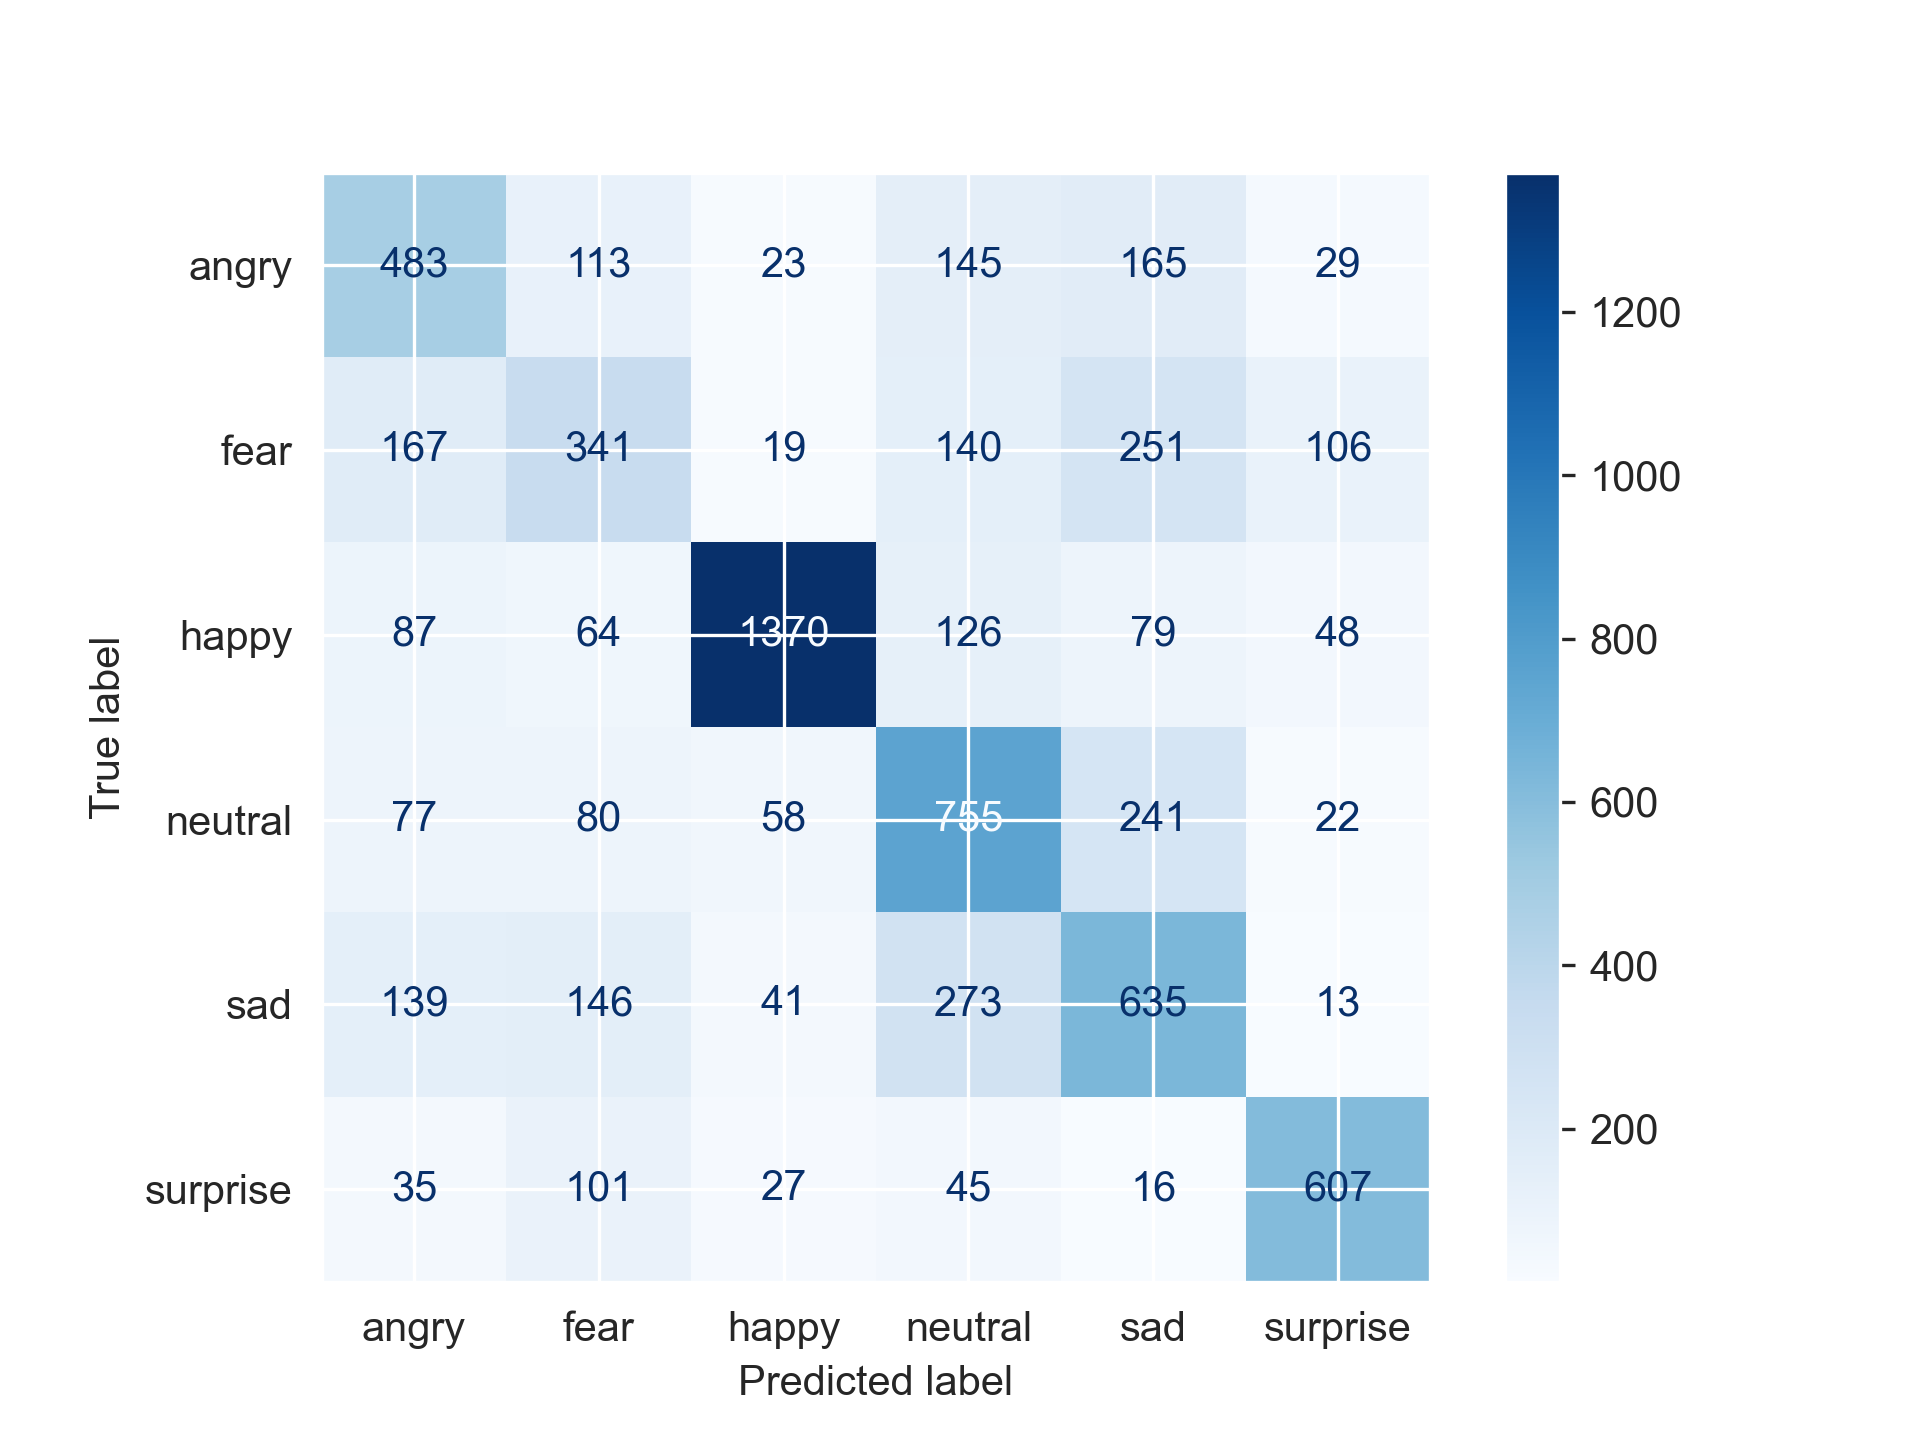
\includegraphics[width=1\textwidth]{figures/cm_efficientnet_b0_trained_02.png}
	\caption{Confusion Matrix - EfficientNet-B0 - post-improvements}
	\label{fig:cm_efficientnet_02}
\end{figure}

\begin{figure}[h]
	\centering
	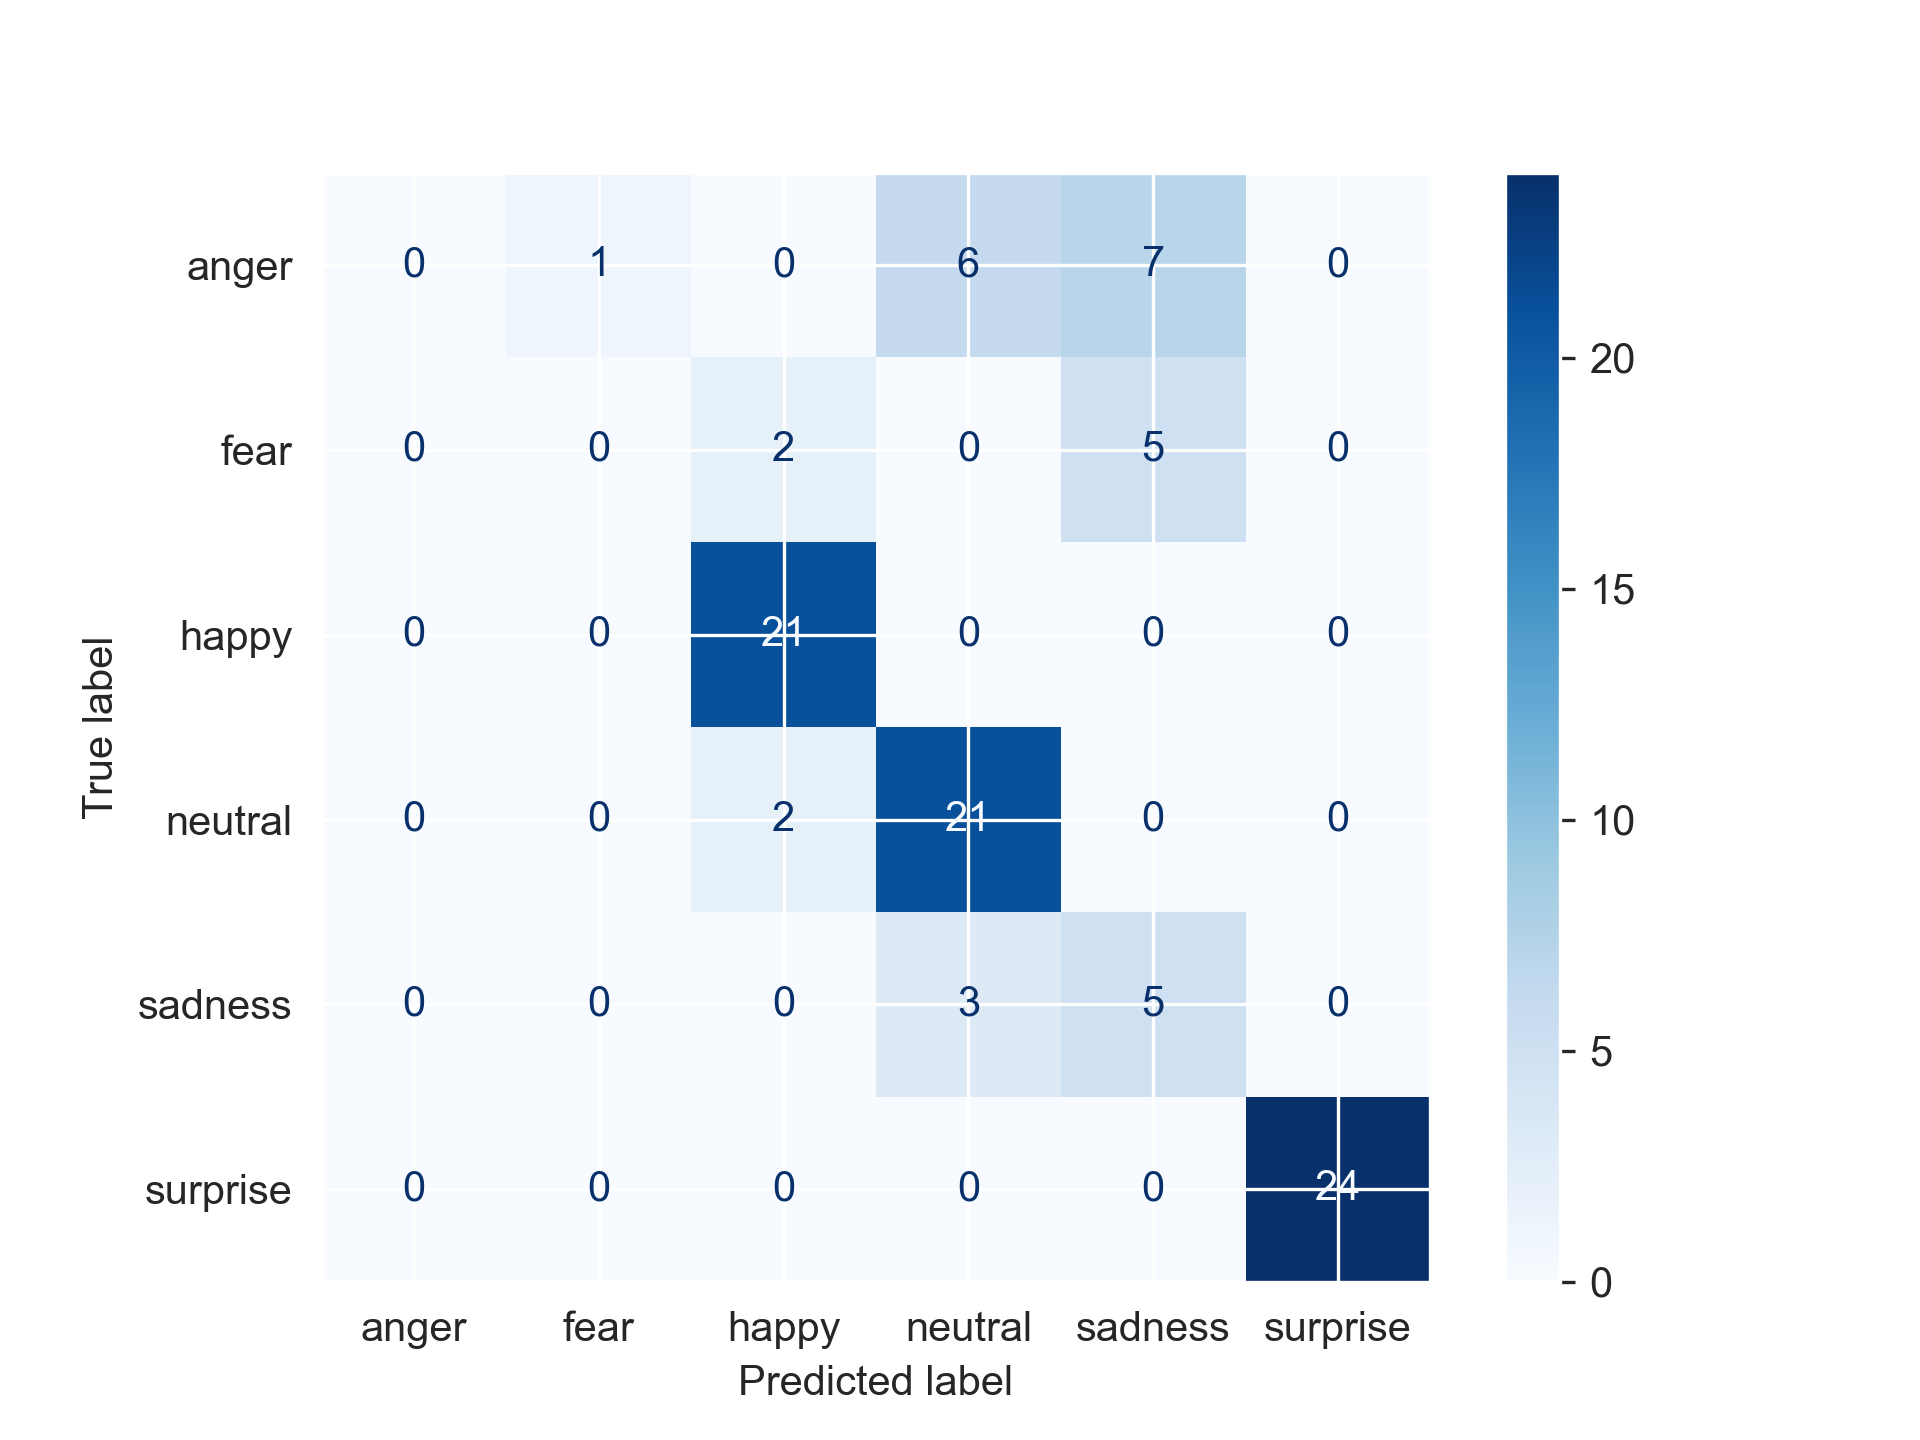
\includegraphics[width=1\textwidth]{figures/cm_efficientnet_b0_trained_ck-dataset.png}
	\caption{Confusion Matrix - EfficientNet-B0 - CK+ Dataset}
	\label{fig:cm_efficientnet_ck}
\end{figure}

\begin{figure}[h]
	\centering
	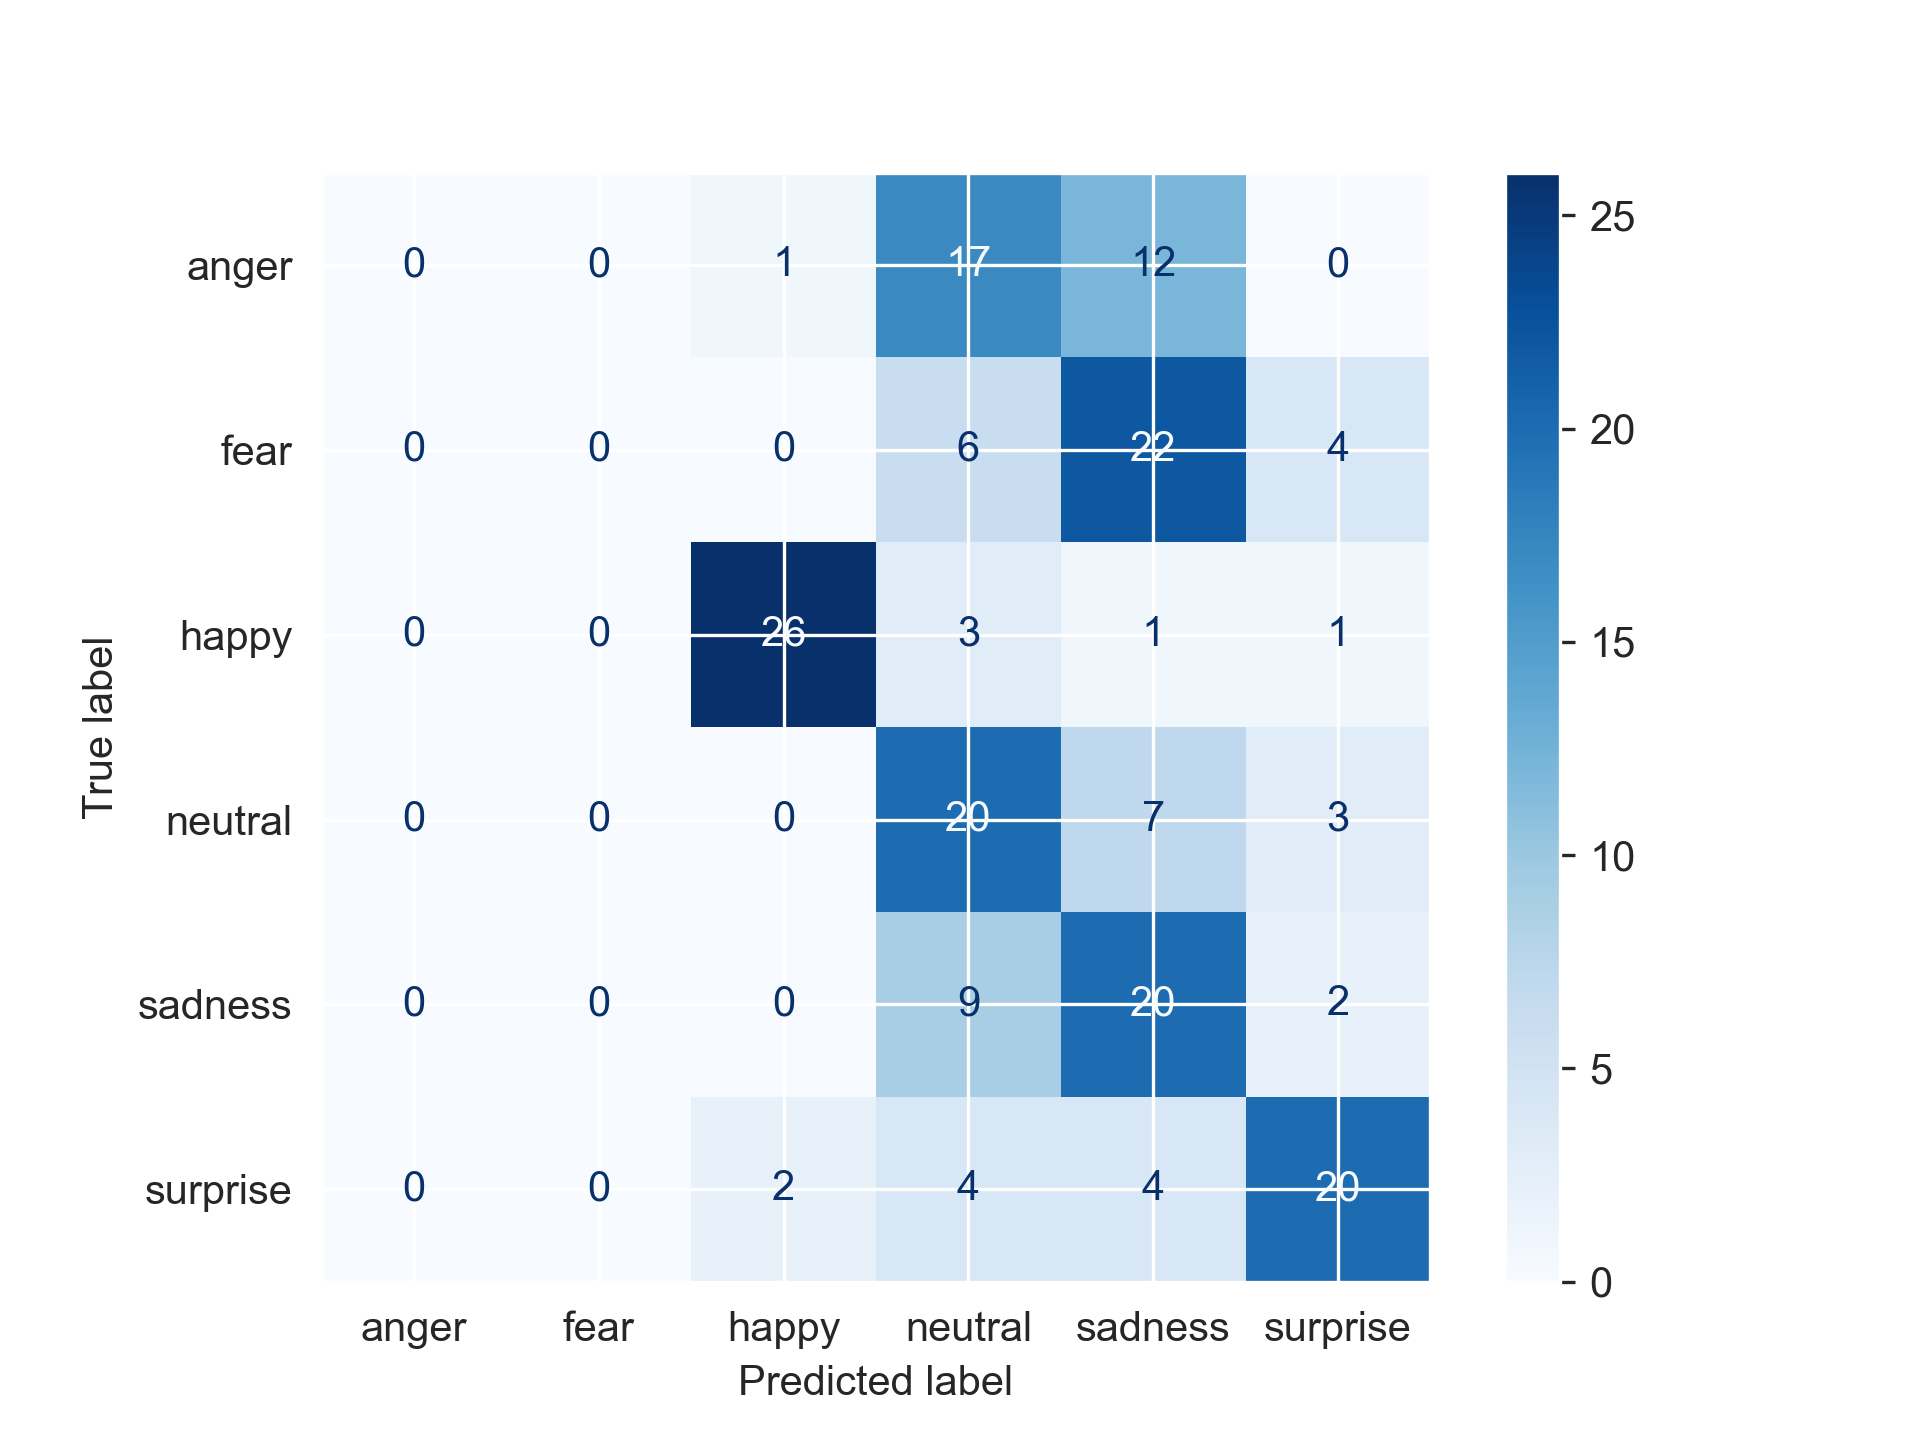
\includegraphics[width=1\textwidth]{figures/cm_efficientnet_b0_trained_jaffe-dataset.png}
	\caption{Confusion Matrix - EfficientNet-B0 - JAFFE Dataset}
	\label{fig:cm_efficientnet_jaffe}
\end{figure}

\begin{figure}[h]
	\centering
	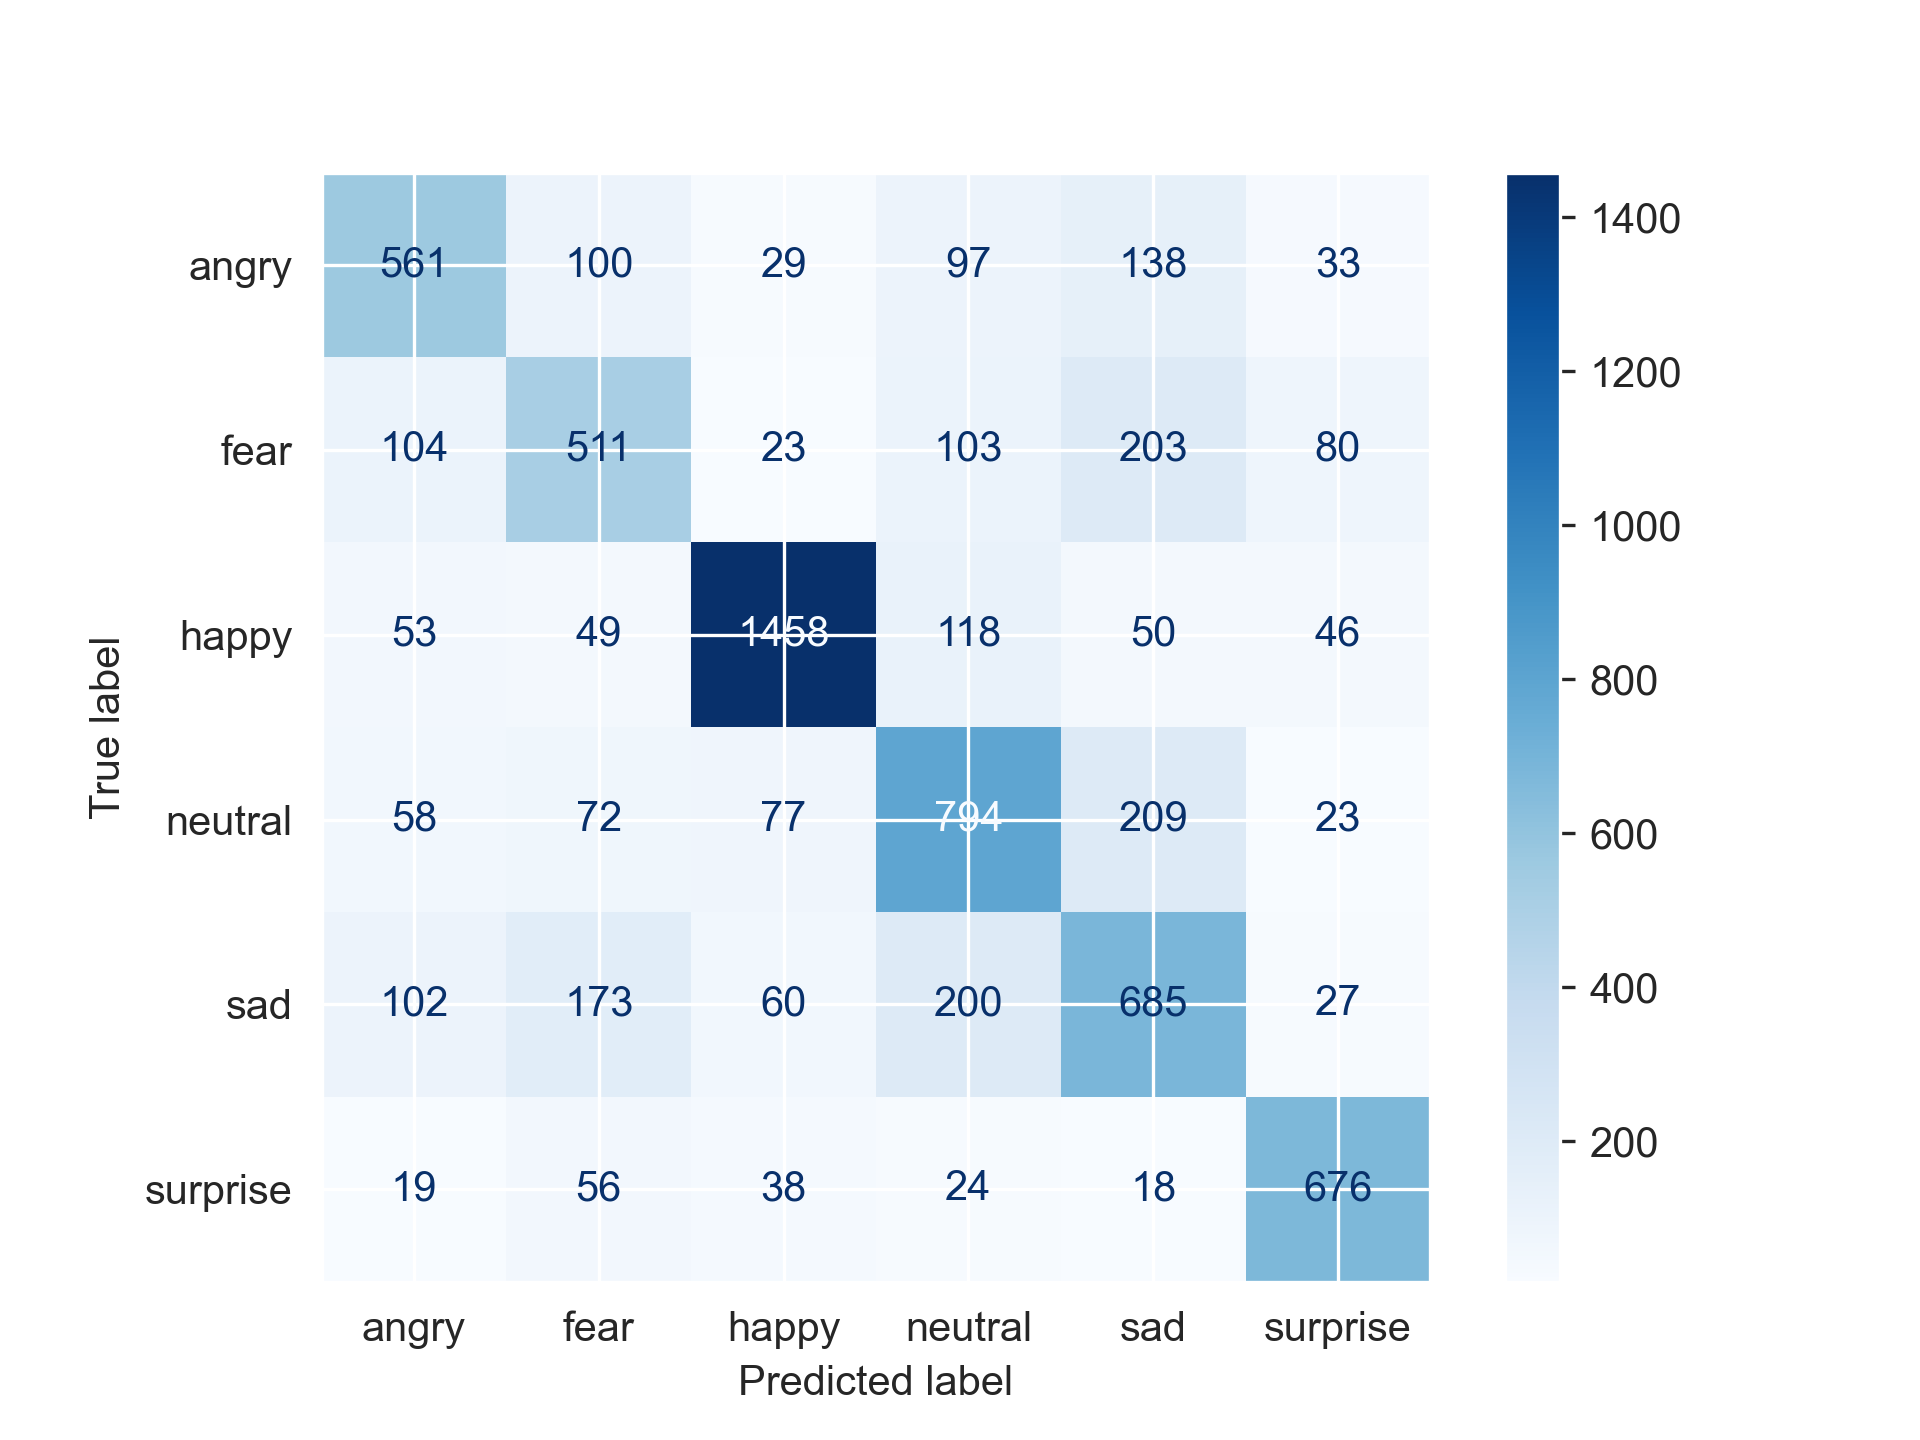
\includegraphics[width=1\textwidth]{figures/cm_resnet_18_trained.png}
	\caption{Confusion Matrix - ResNet18 - pre-improvements}
	\label{fig:cm_resnet_01}
\end{figure}

\begin{figure}[h]
	\centering
	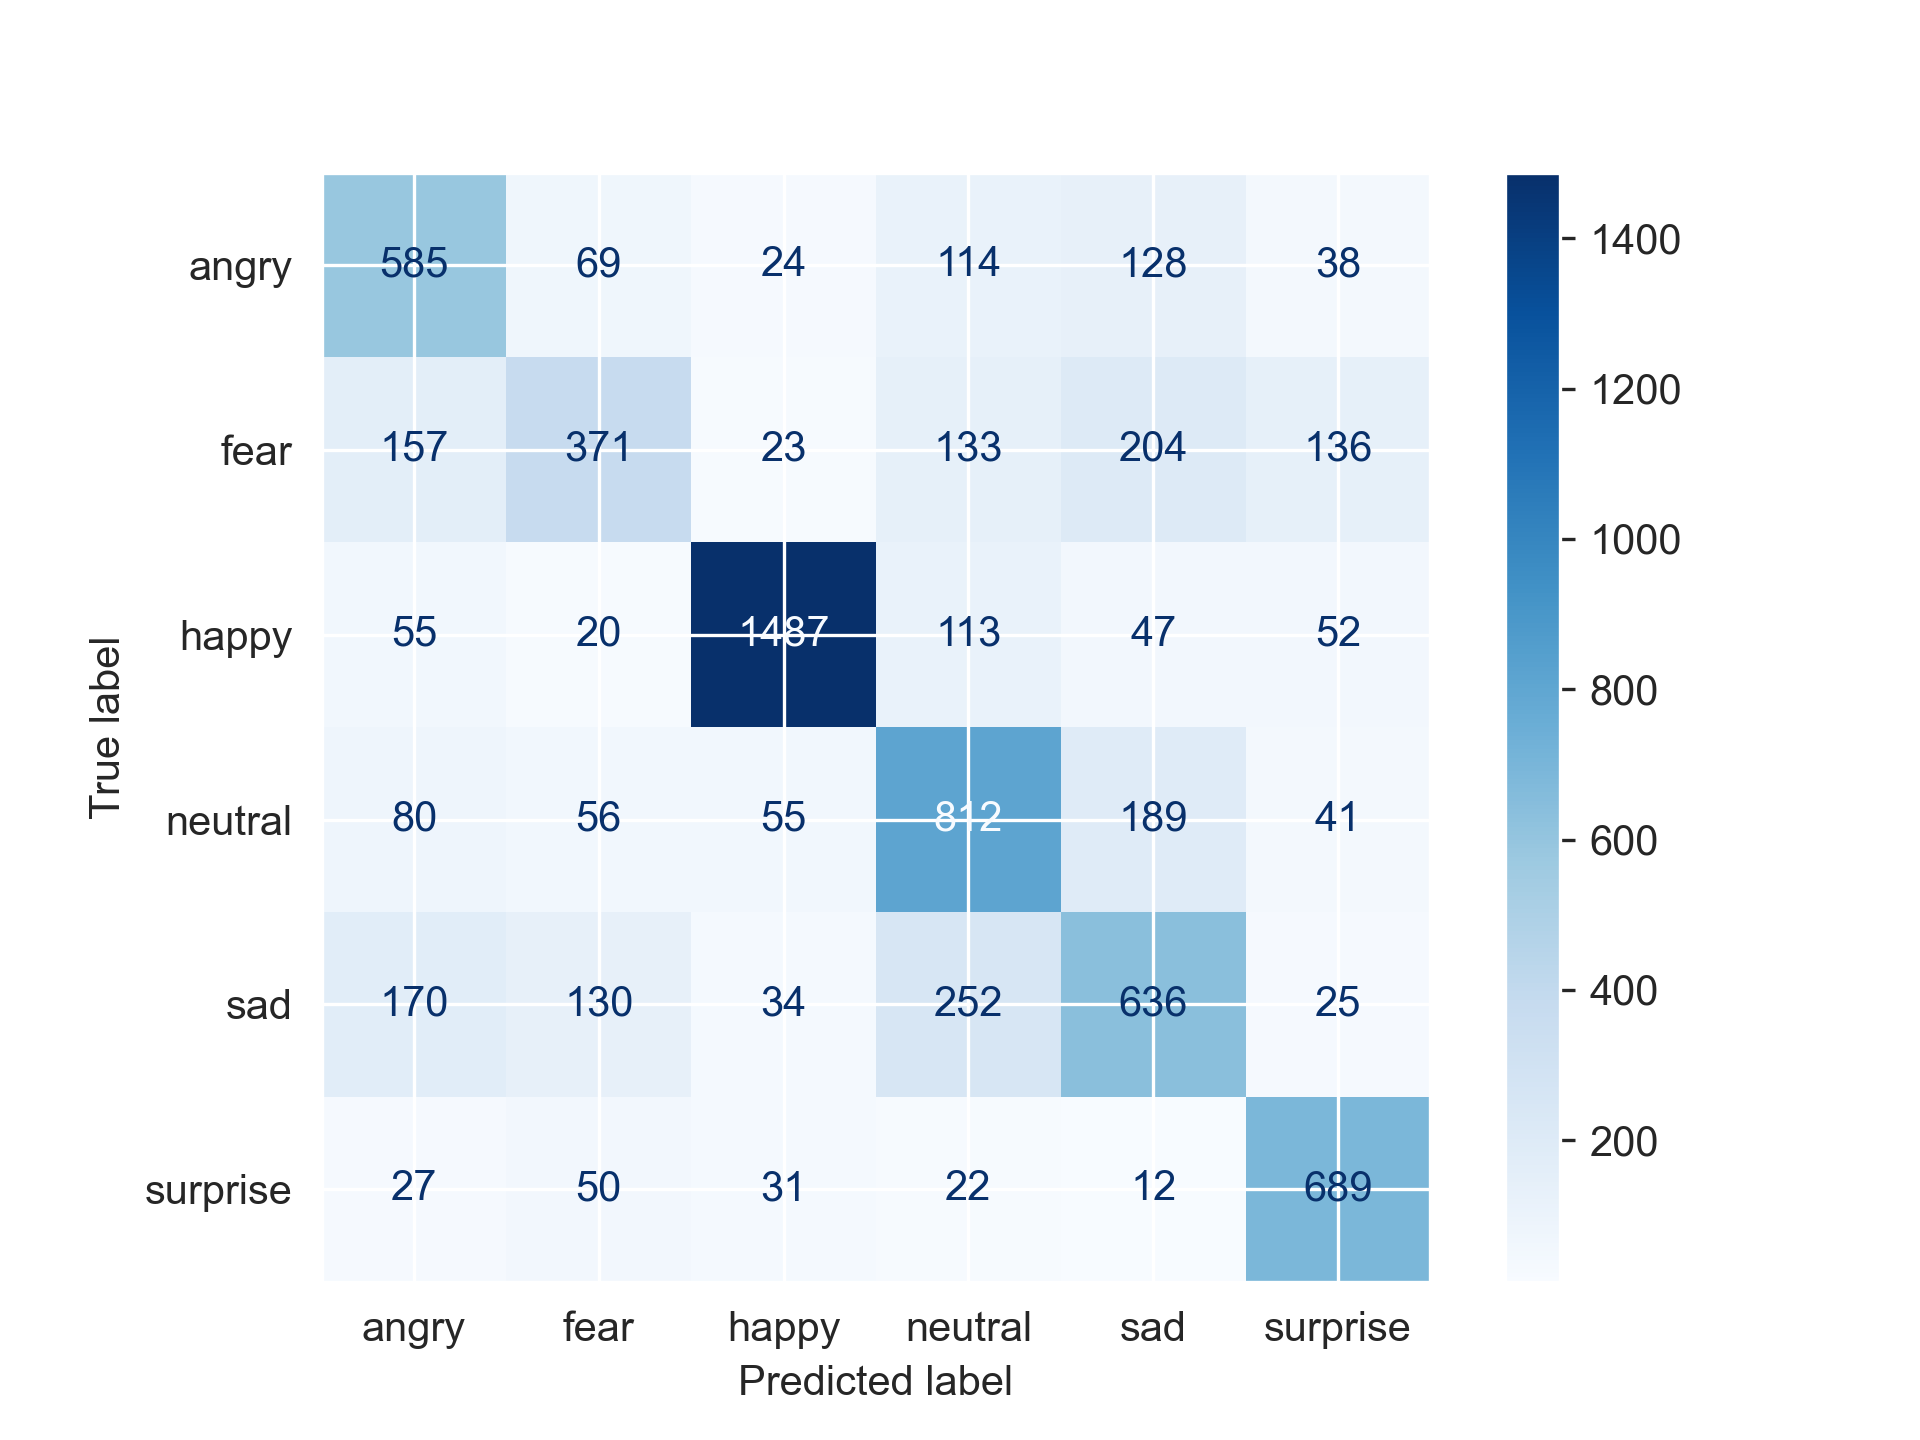
\includegraphics[width=1\textwidth]{figures/cm_resnet_18_trained_02.png}
	\caption{Confusion Matrix - ResNet18 - post-improvements}
	\label{fig:cm_resnet_02}
\end{figure}

\begin{figure}[h]
	\centering
	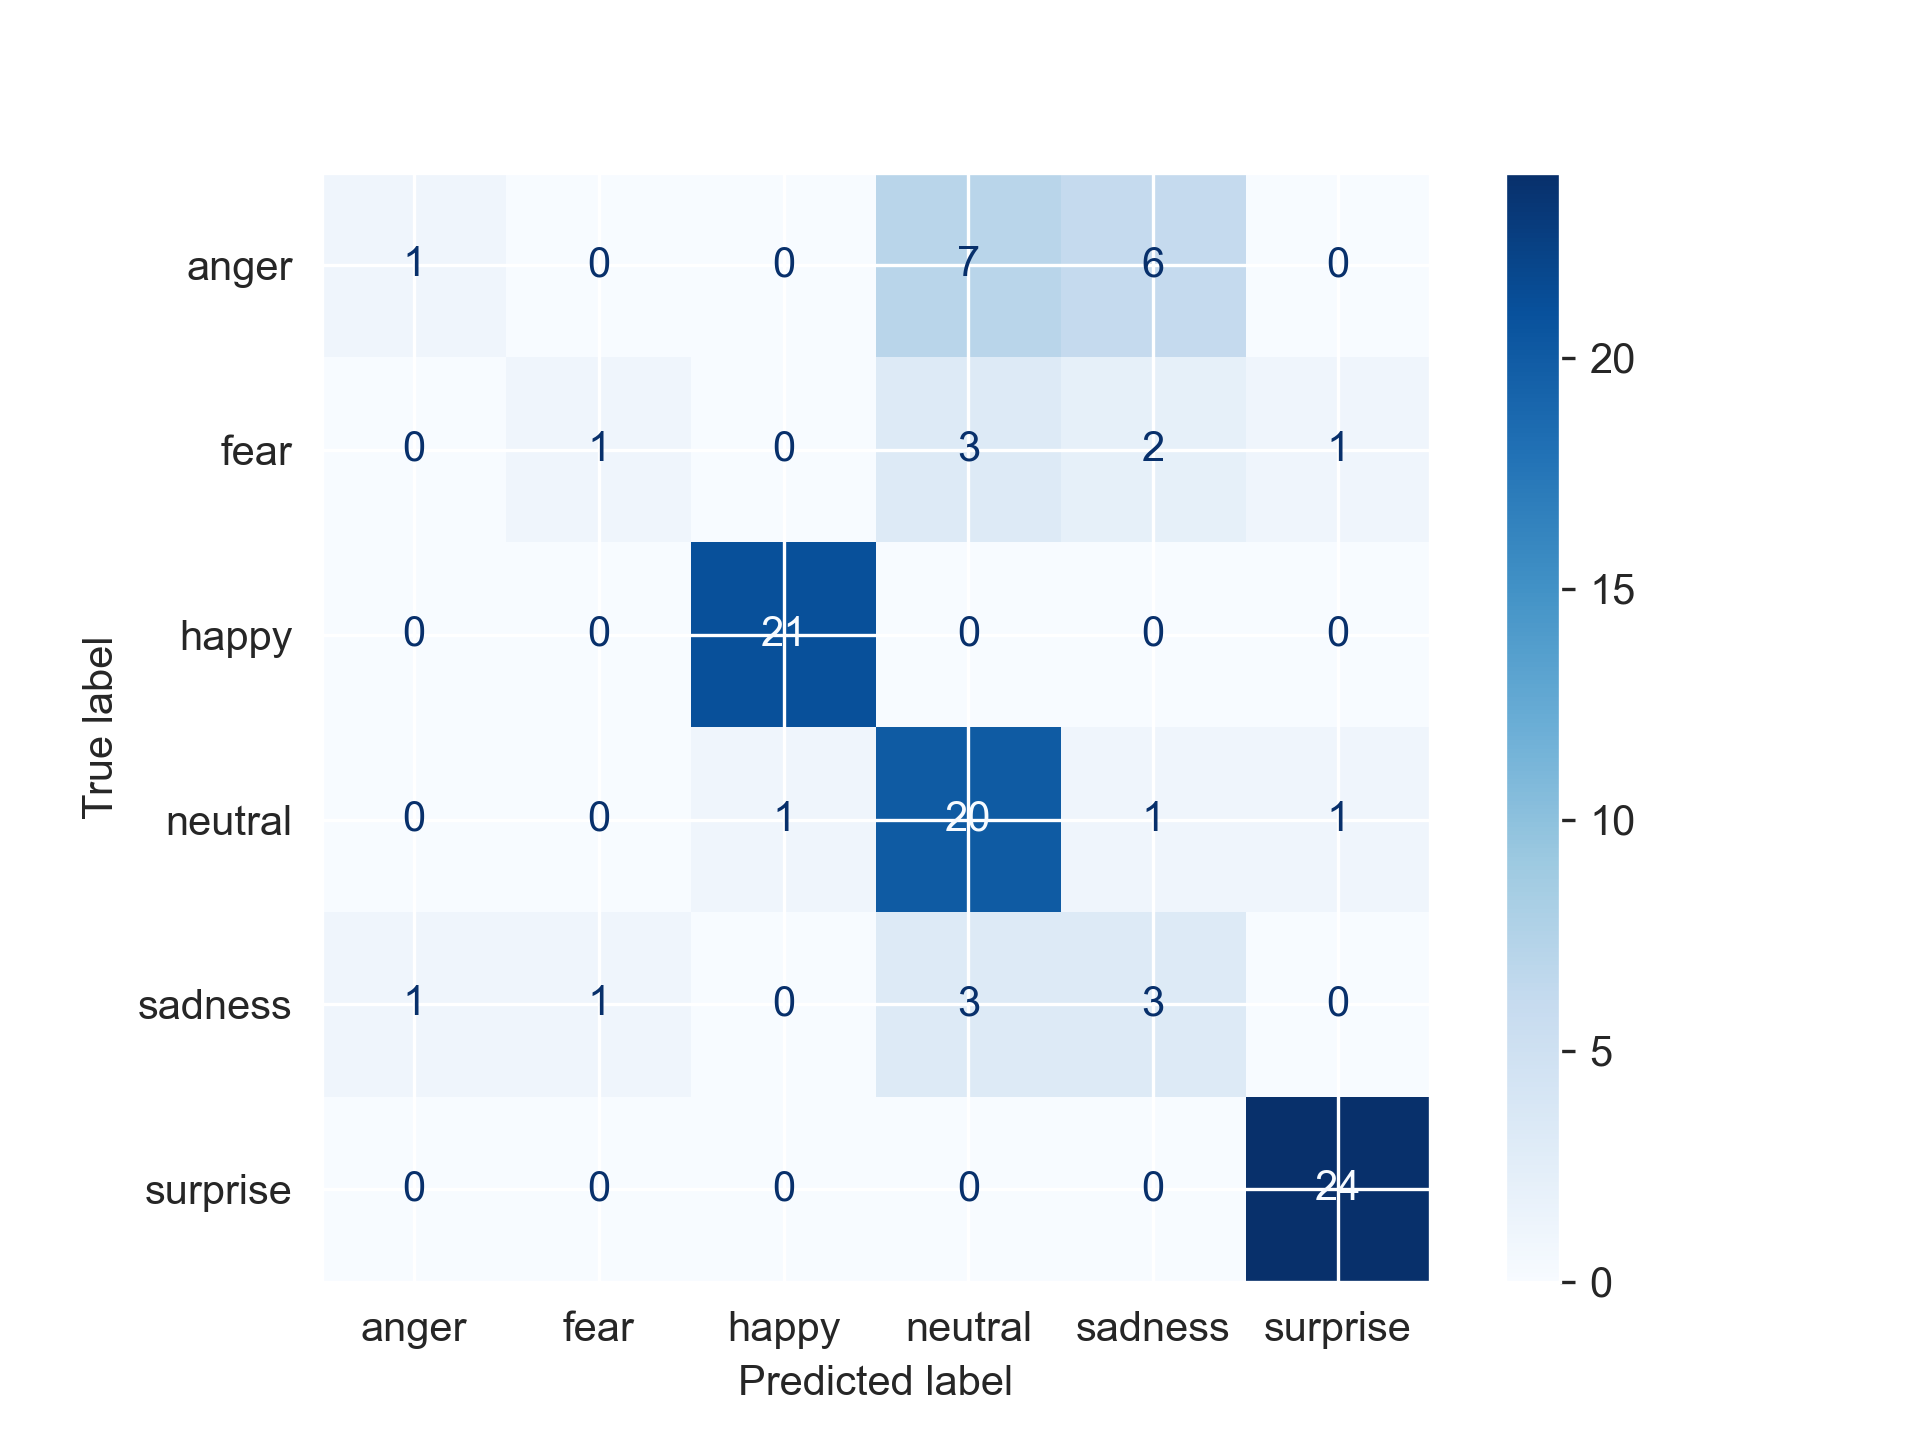
\includegraphics[width=1\textwidth]{figures/cm_resnet_18_trained_ck-dataset.png}
	\caption{Confusion Matrix - ResNet18 - CK+ Dataset}
	\label{fig:cm_resnet_ck}
\end{figure}

\begin{figure}[h]
	\centering
	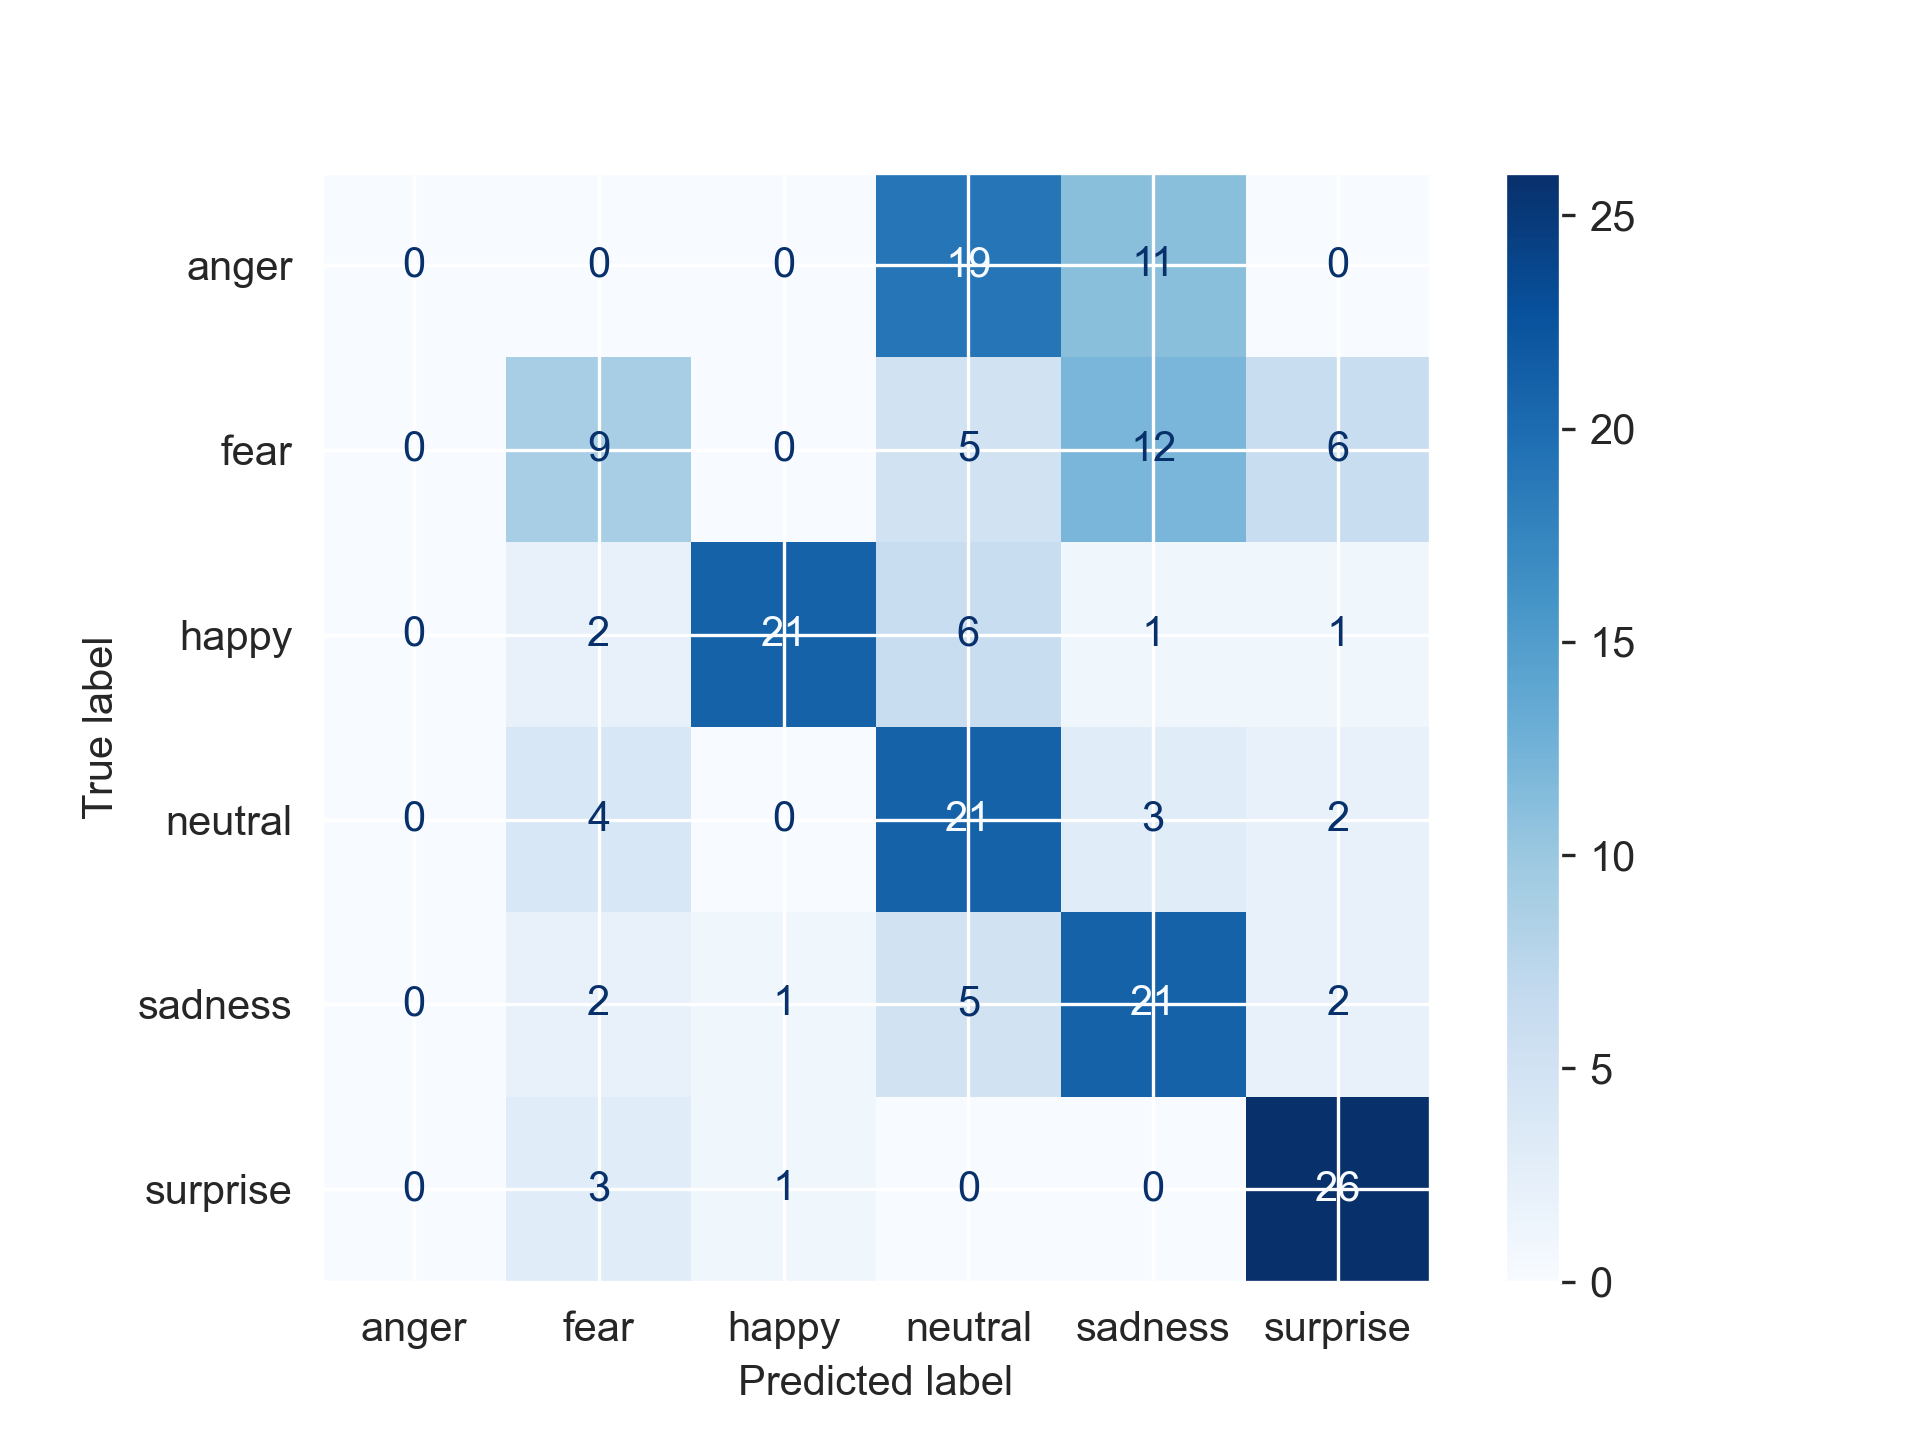
\includegraphics[width=1\textwidth]{figures/cm_resnet_18_trained_jaffe-dataset.png}
	\caption{Confusion Matrix - ResNet18 - JAFFE Dataset}
	\label{fig:cm_resnet_jaffe}
\end{figure}

\begin{figure}[h]
	\centering
	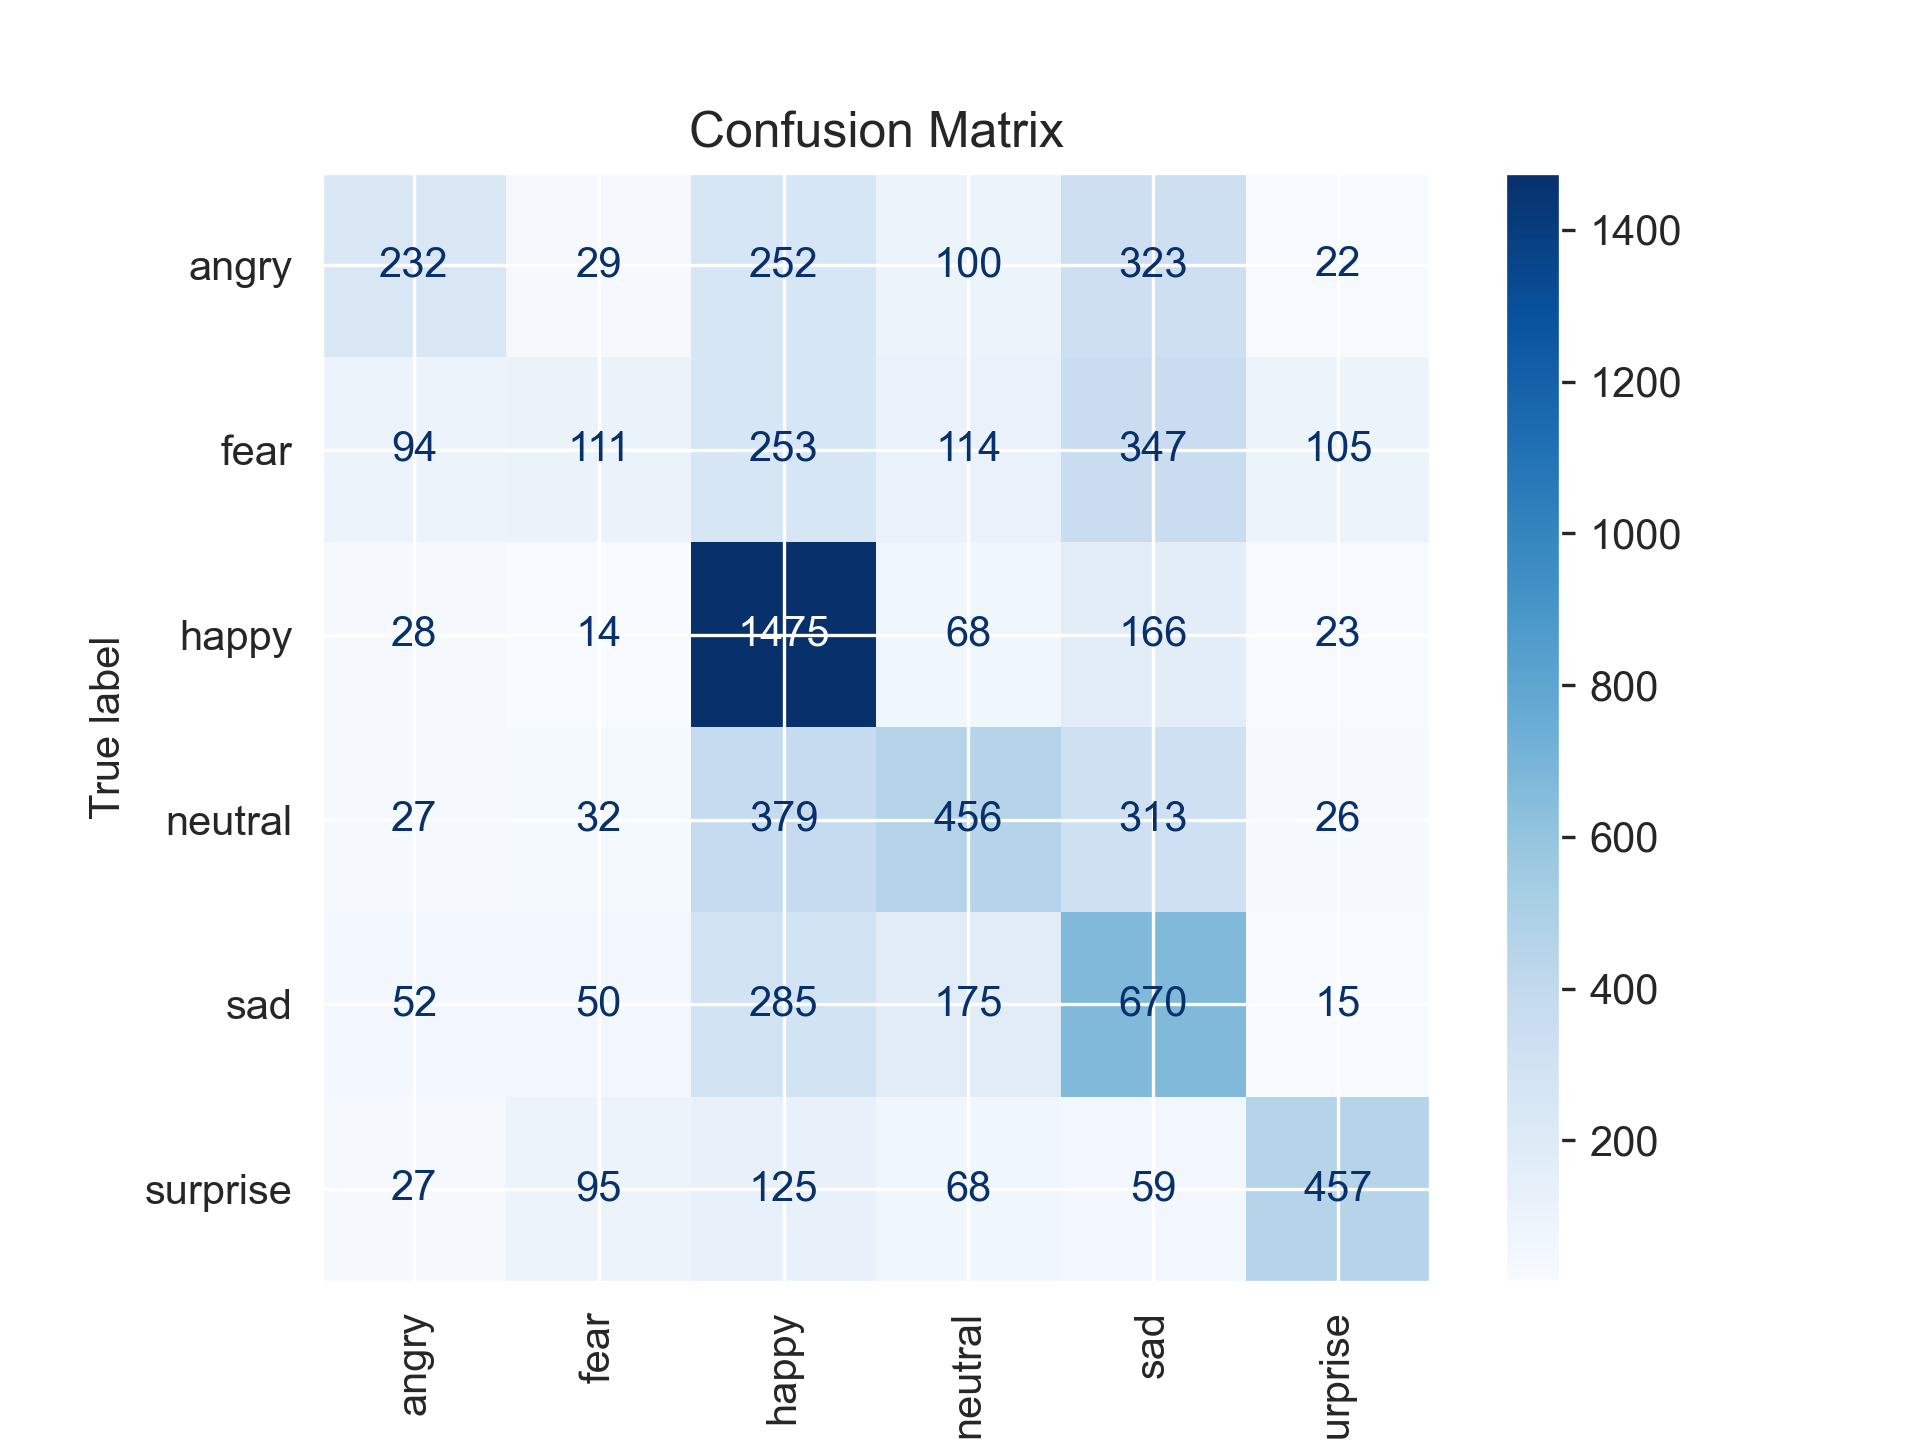
\includegraphics[width=1\textwidth]{figures/conf_matrix_vgg16.png}
	\caption{Confusion Matrix - VGG16}
	\label{fig:cm_vgg16}
\end{figure}

\begin{figure}[h]
	\centering
	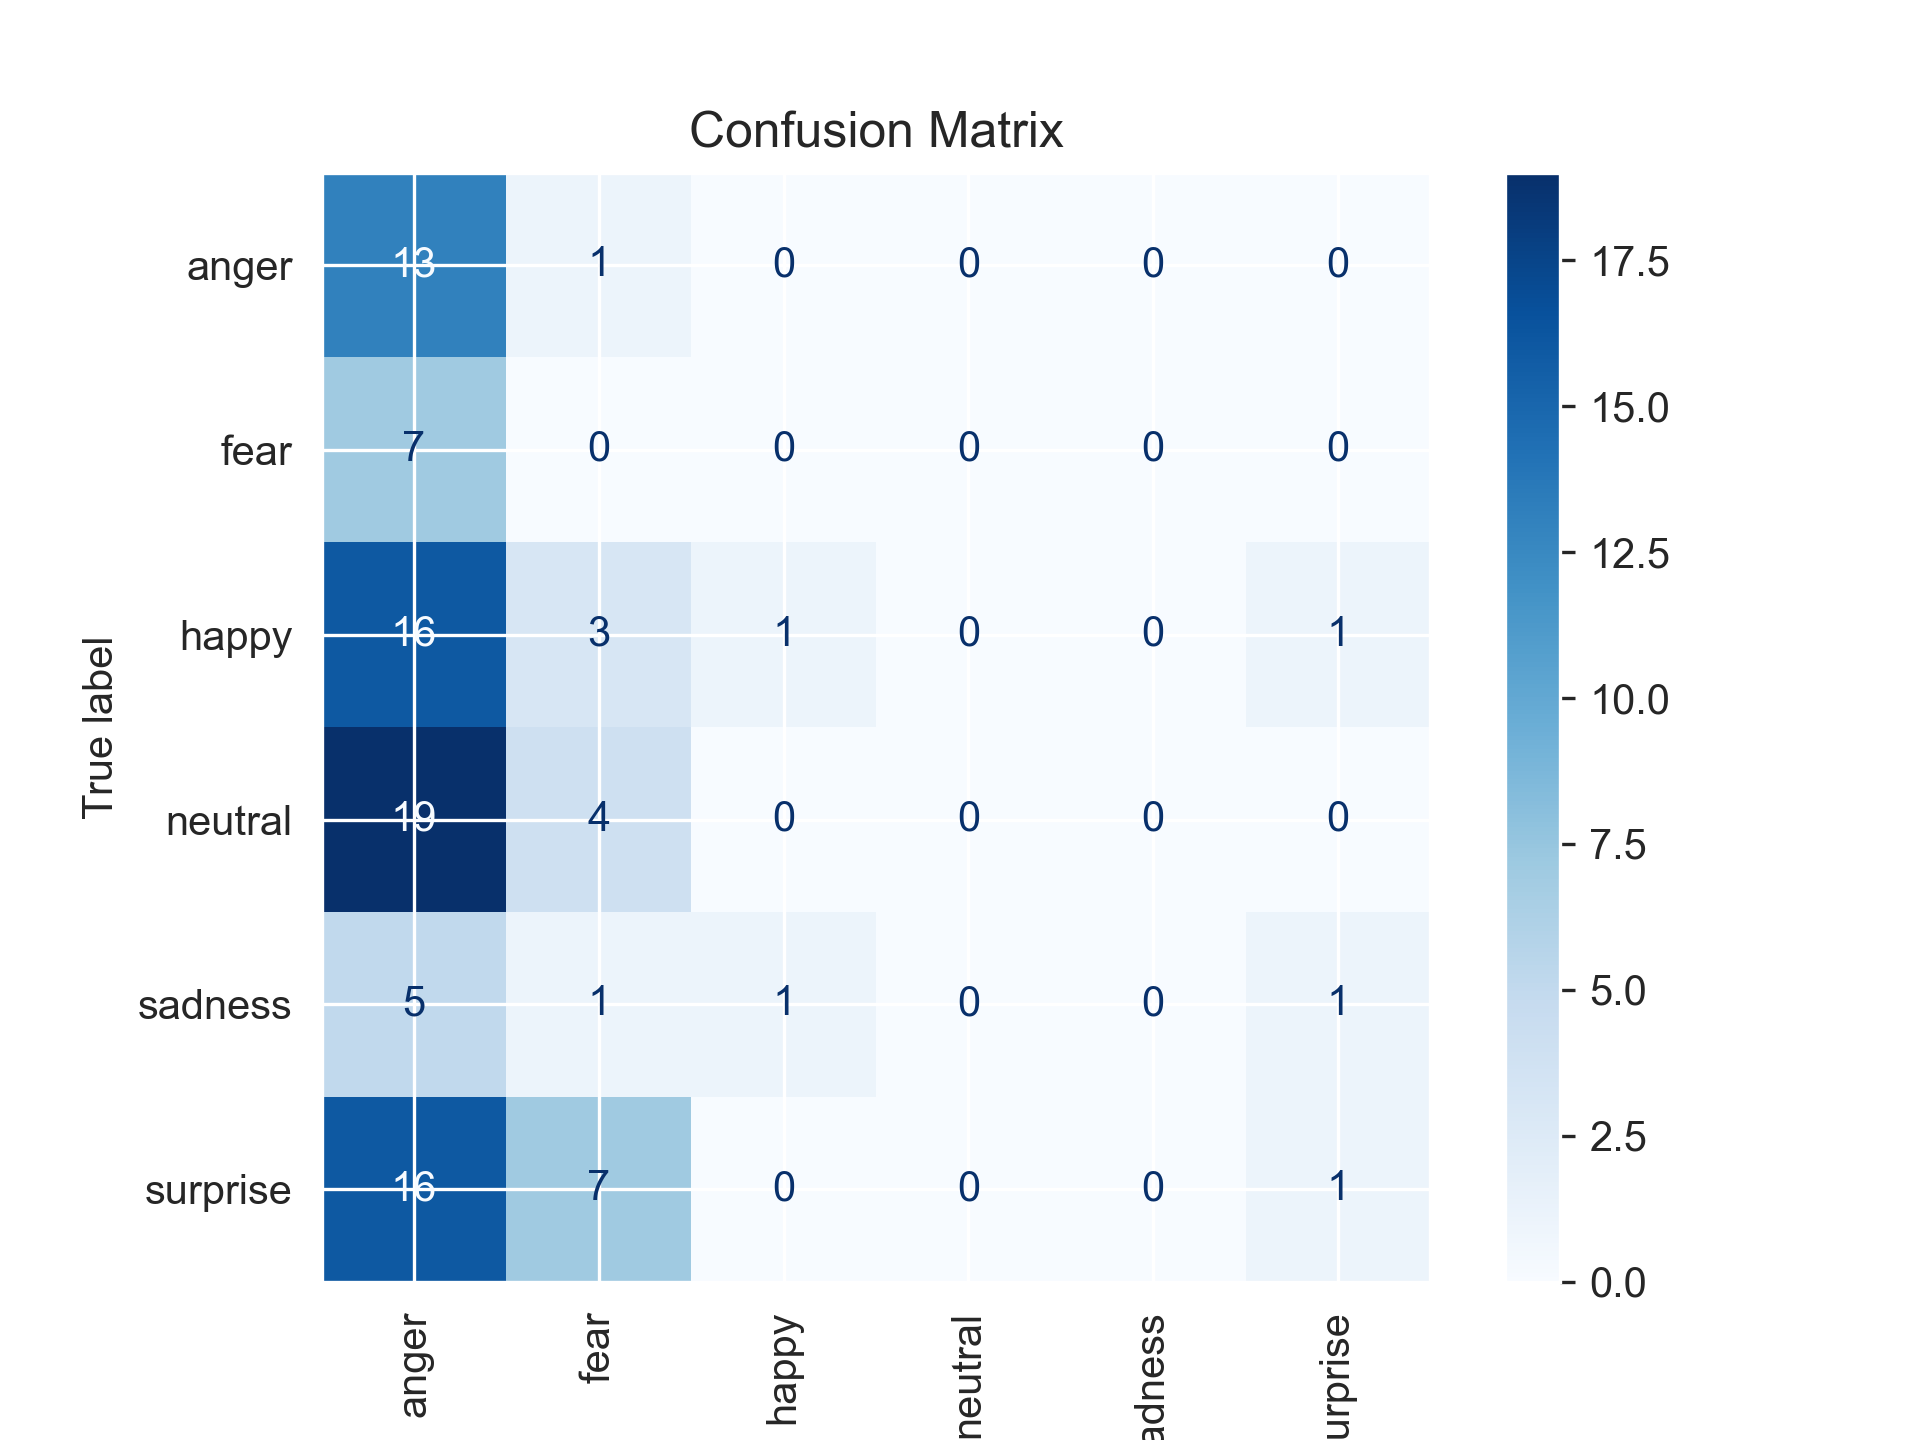
\includegraphics[width=1\textwidth]{figures/conf_matrix_vgg16_ck-dataset.png}
	\caption{Confusion Matrix - VGG16 - CK+ Dataset}
	\label{fig:cm_vgg16_ck}
\end{figure}

\begin{figure}[h]
	\centering
	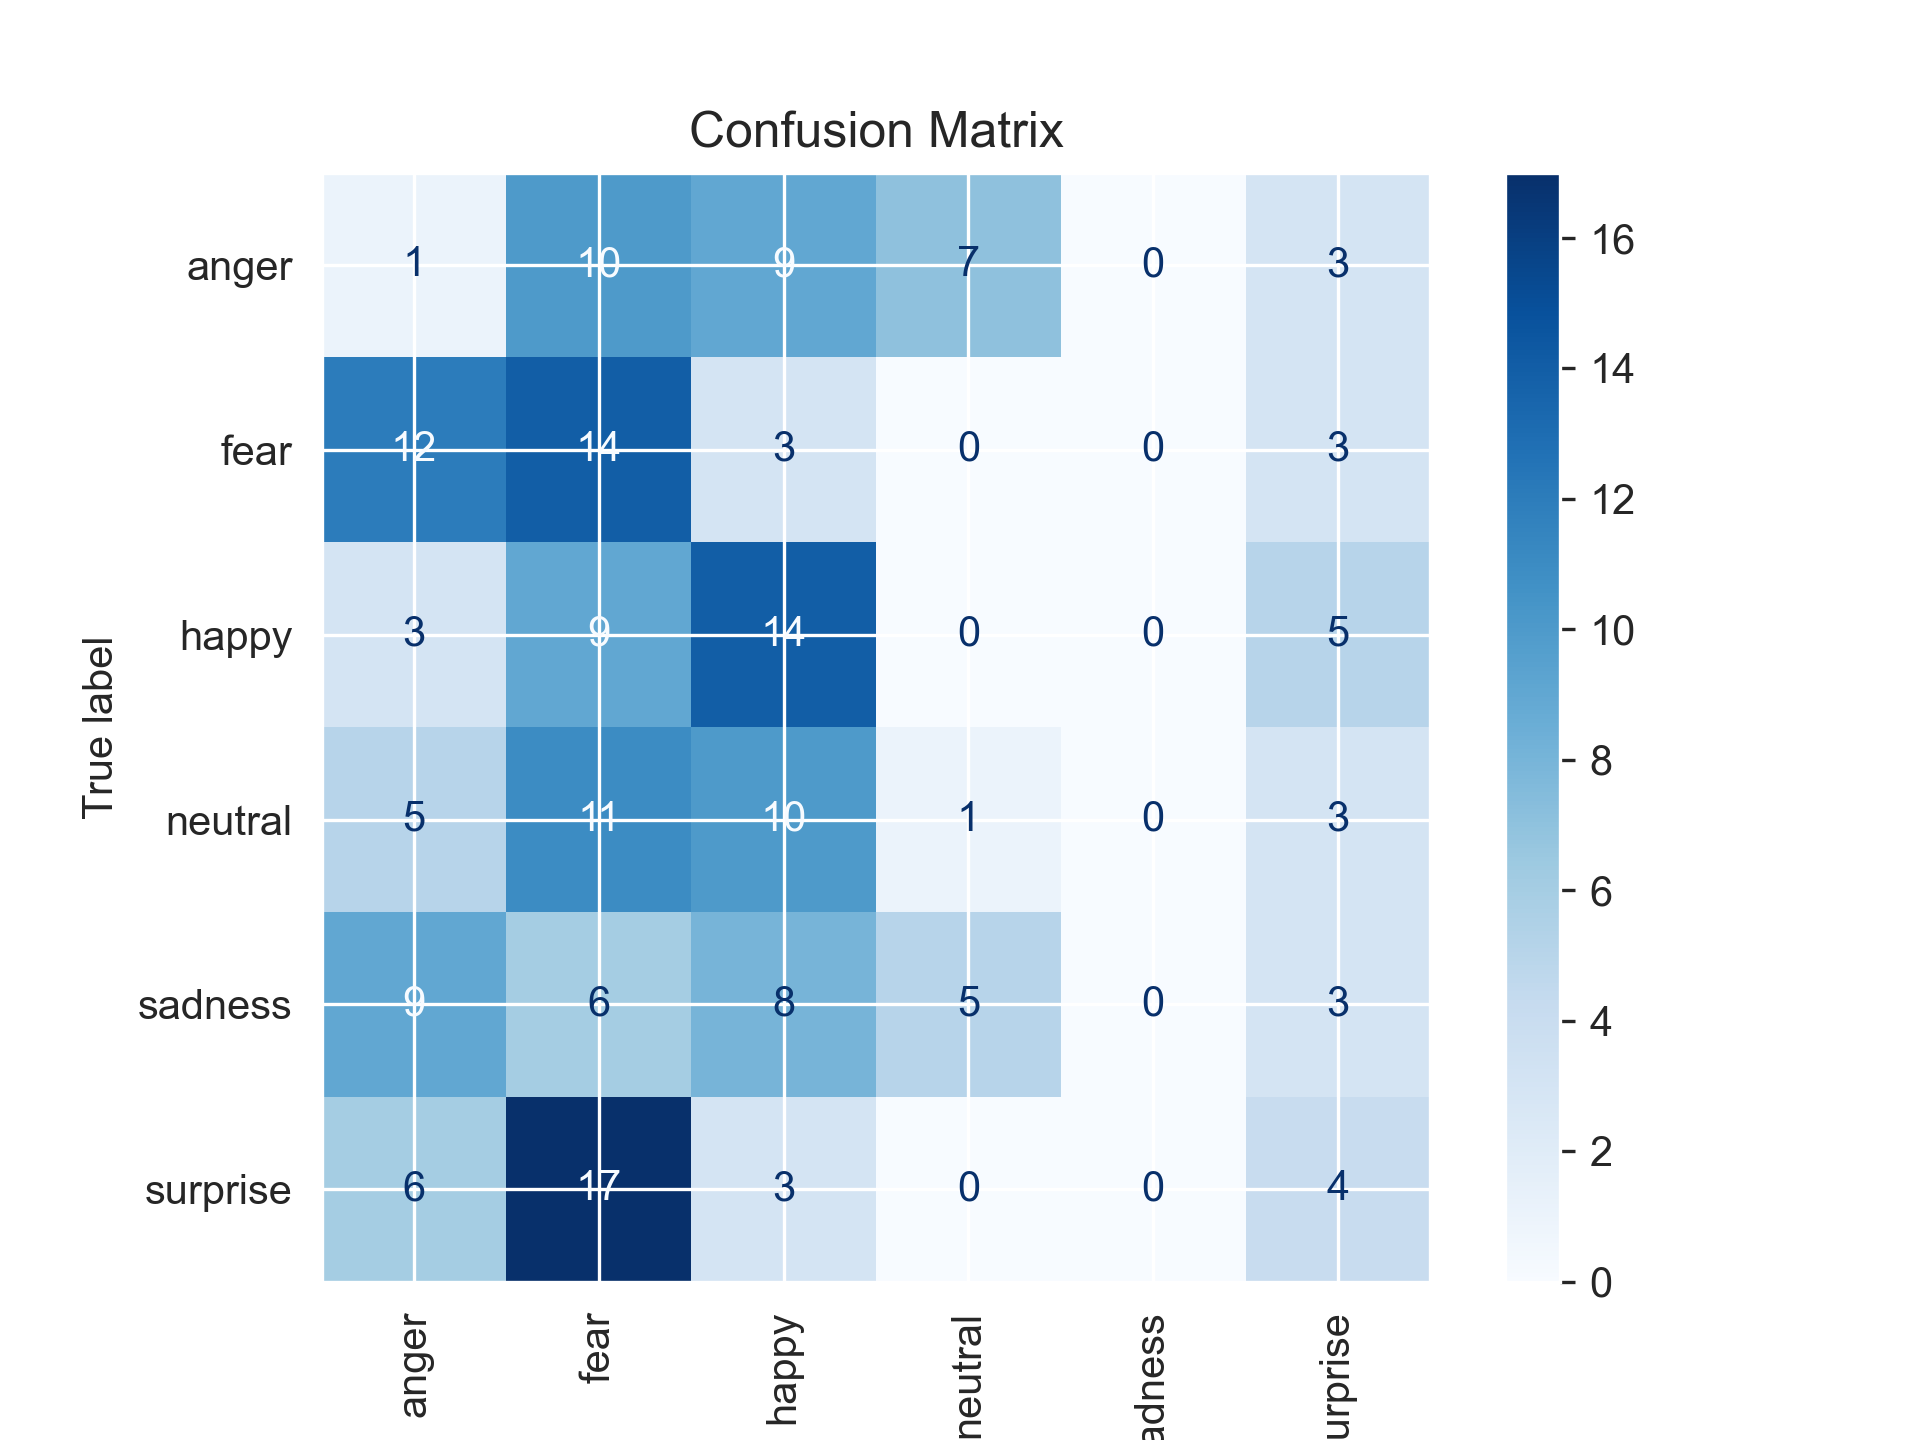
\includegraphics[width=1\textwidth]{figures/conf_matrix_vgg16_jaffe-dataset.png}
	\caption{Confusion Matrix - VGG16 - JAFFE Dataset}
	\label{fig:cm_vgg16_jaffe}
\end{figure}

\chapter{Classification Reports}
\label{cr}

\begin{figure}[h]
	\begin{subfigure}{0.5\textwidth}
		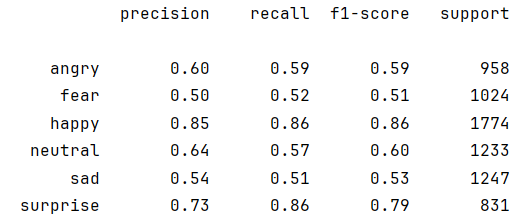
\includegraphics[width=0.9\linewidth]{figures/efficientnet_cr_01.png} 
		\caption{Results for FER-2013 - pre-improvements}
		\label{fig:subim1}
	\end{subfigure}
	\begin{subfigure}{0.5\textwidth}
		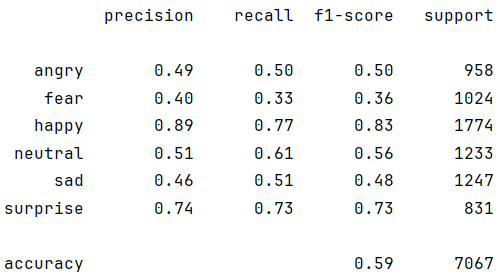
\includegraphics[width=0.9\linewidth]{figures/efficientnet_cr_02.png}
		\caption{Results for FER-2013 - post-improvements}
		\label{fig:subim2}
	\end{subfigure}
	
	\begin{subfigure}{0.5\textwidth}
		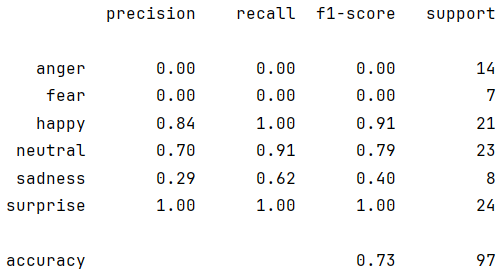
\includegraphics[width=0.9\linewidth]{figures/efficientnet_cr_ck-dataset.png} 
		\caption{Results for CK+ Dataset}
		\label{fig:subim3}
	\end{subfigure}
	\begin{subfigure}{0.5\textwidth}
		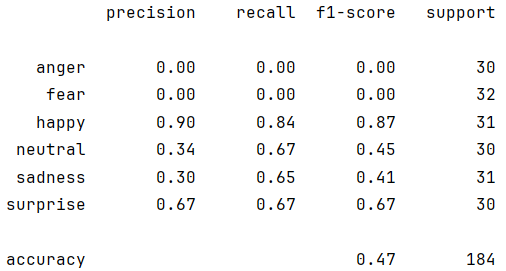
\includegraphics[width=0.9\linewidth]{figures/efficientnet_cr_jaffe-dataset.png}
		\caption{Results for JAFFE Dataset}
		\label{fig:subim4}
	\end{subfigure}
	
	\caption{Classification Reports for EfficientNet-B0 Model}
	\label{fig:image2}
\end{figure}

\begin{figure}[h]
	\begin{subfigure}{0.5\textwidth}
		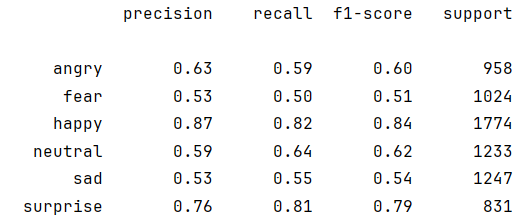
\includegraphics[width=0.9\linewidth]{figures/resnet_cr_01.png} 
		\caption{Results for FER-2013 - pre-improvements}
		\label{fig:subim5}
	\end{subfigure}
	\begin{subfigure}{0.5\textwidth}
		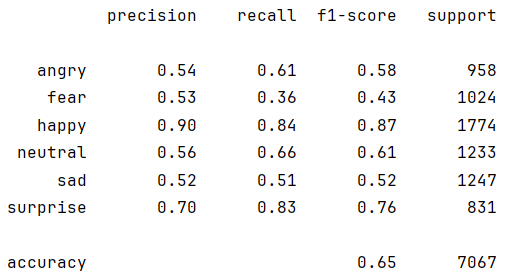
\includegraphics[width=0.9\linewidth]{figures/resnet_cr_02.png}
		\caption{Results for FER-2013 - post-improvements}
		\label{fig:subim6}
	\end{subfigure}
	
	\begin{subfigure}{0.5\textwidth}
		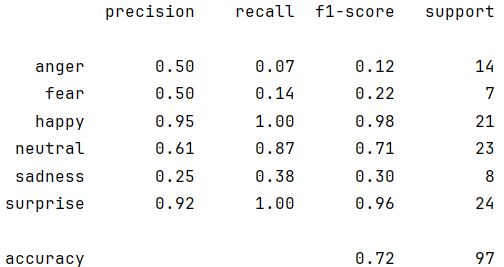
\includegraphics[width=0.9\linewidth]{figures/resnet_cr_ck-dataset.png} 
		\caption{Results for CK+ Dataset}
		\label{fig:subim7}
	\end{subfigure}
	\begin{subfigure}{0.5\textwidth}
		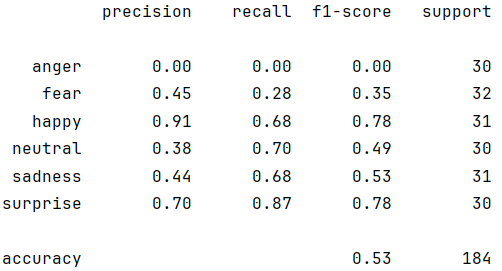
\includegraphics[width=0.9\linewidth]{figures/resnet_cr_jaffe-dataset.png}
		\caption{Results for JAFFE Dataset}
		\label{fig:subim8}
	\end{subfigure}
	
	\caption{Classification Reports for ResNet-18 Model}
	\label{fig:image3}
\end{figure}

\begin{figure}[h]
	\begin{subfigure}{0.5\textwidth}
		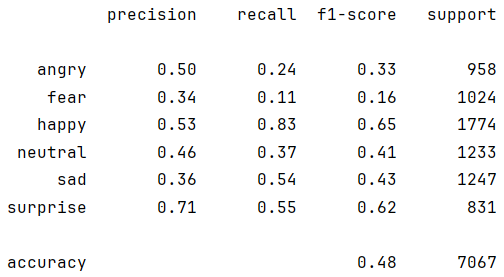
\includegraphics[width=0.9\linewidth]{figures/vgg16_cr_01.png} 
		\caption{Results for FER-2013}
		\label{fig:subim9}
	\end{subfigure}
	\begin{subfigure}{0.5\textwidth}
		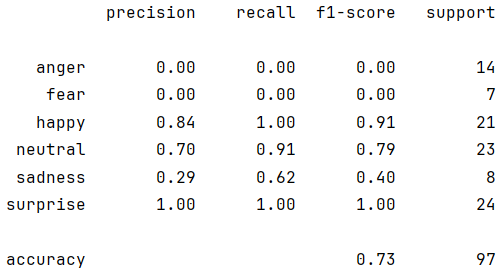
\includegraphics[width=0.9\linewidth]{figures/vgg16_cr_ck-dataset.png} 
		\caption{Results for CK+ Dataset}
		\label{fig:subim91}
	\end{subfigure}
	\begin{subfigure}{0.5\textwidth}
		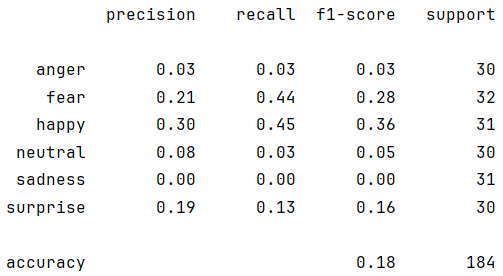
\includegraphics[width=0.9\linewidth]{figures/vgg16_cr_jaffe-dataset.png}
		\caption{Results for JAFFE Dataset}
		\label{fig:subim92}
	\end{subfigure}
	
	\caption{Classification Reports for VGG16 Model}
	\label{fig:image4}
\end{figure}

\chapter{Predictions}
\label{predictions}

%\begin{figure}[h]
%	\centering
%	\includegraphics[width=1\textwidth]{figures/Emotions.png}
%	\caption{Display of Emotions}
%	\label{fig:emotions}
%\end{figure}

\begin{figure}[h]
	\centering
	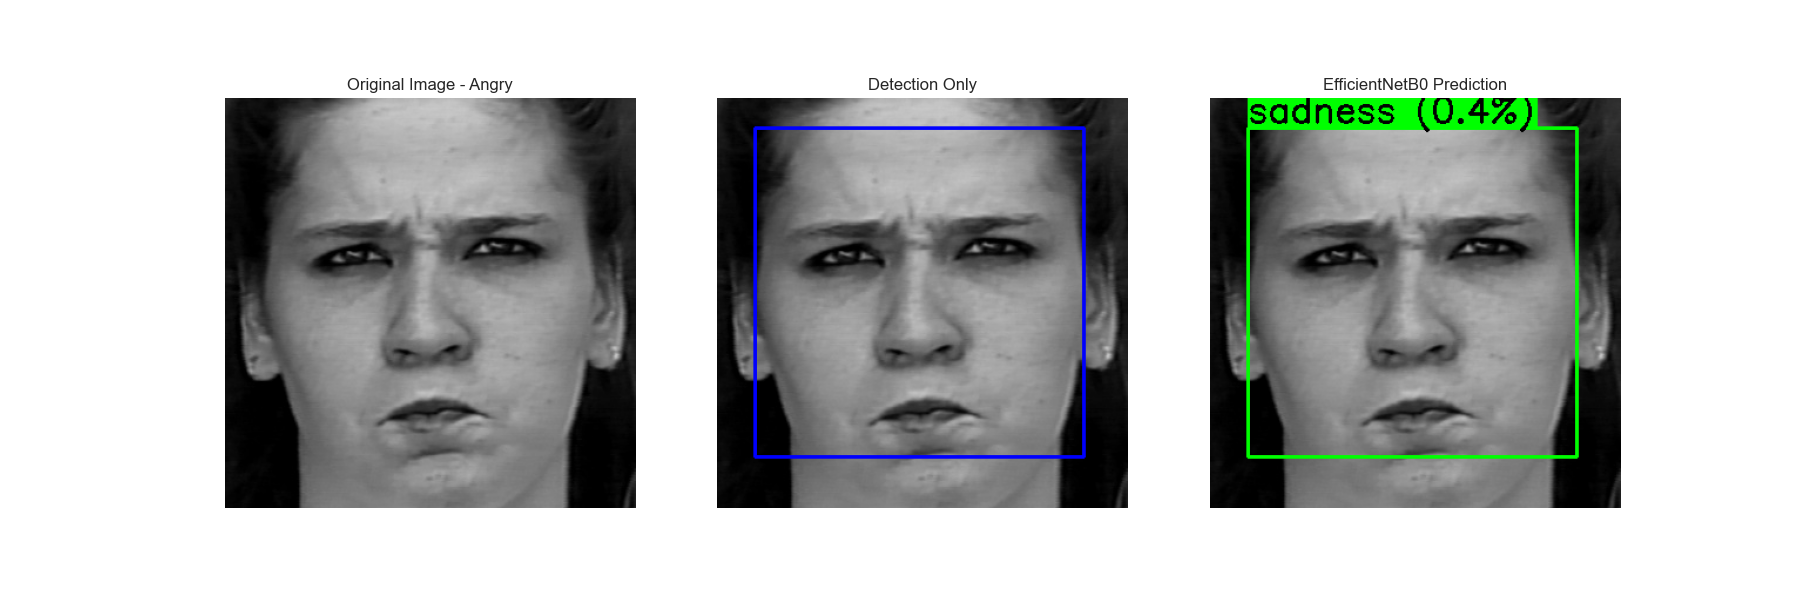
\includegraphics[width=1\textwidth]{figures/EfficientNetB0_Angry.png}
	\caption{Prediction - EfficientNet-B0 - Emotion: "Angry", Predicted: "Sadness"}
	\label{fig:predictions_efficientnet_01}
\end{figure}

\begin{figure}[h]
	\centering
	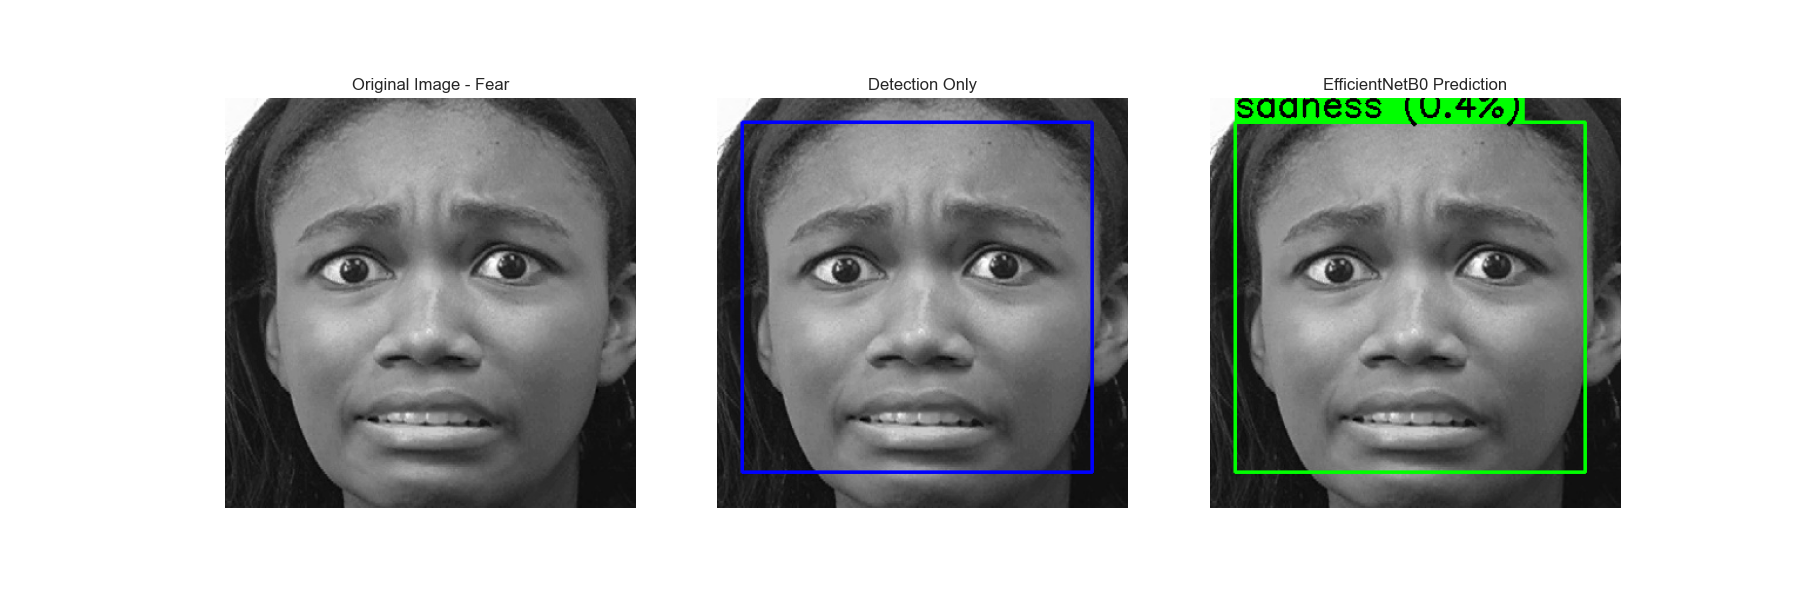
\includegraphics[width=1\textwidth]{figures/EfficientNetB0_Fear.png}
	\caption{Prediction - EfficientNet-B0 - Emotion: "Fear", Predicted: "Sadness"}
	\label{fig:predictions_efficientnet_02}
\end{figure}

\begin{figure}[h]
	\centering
	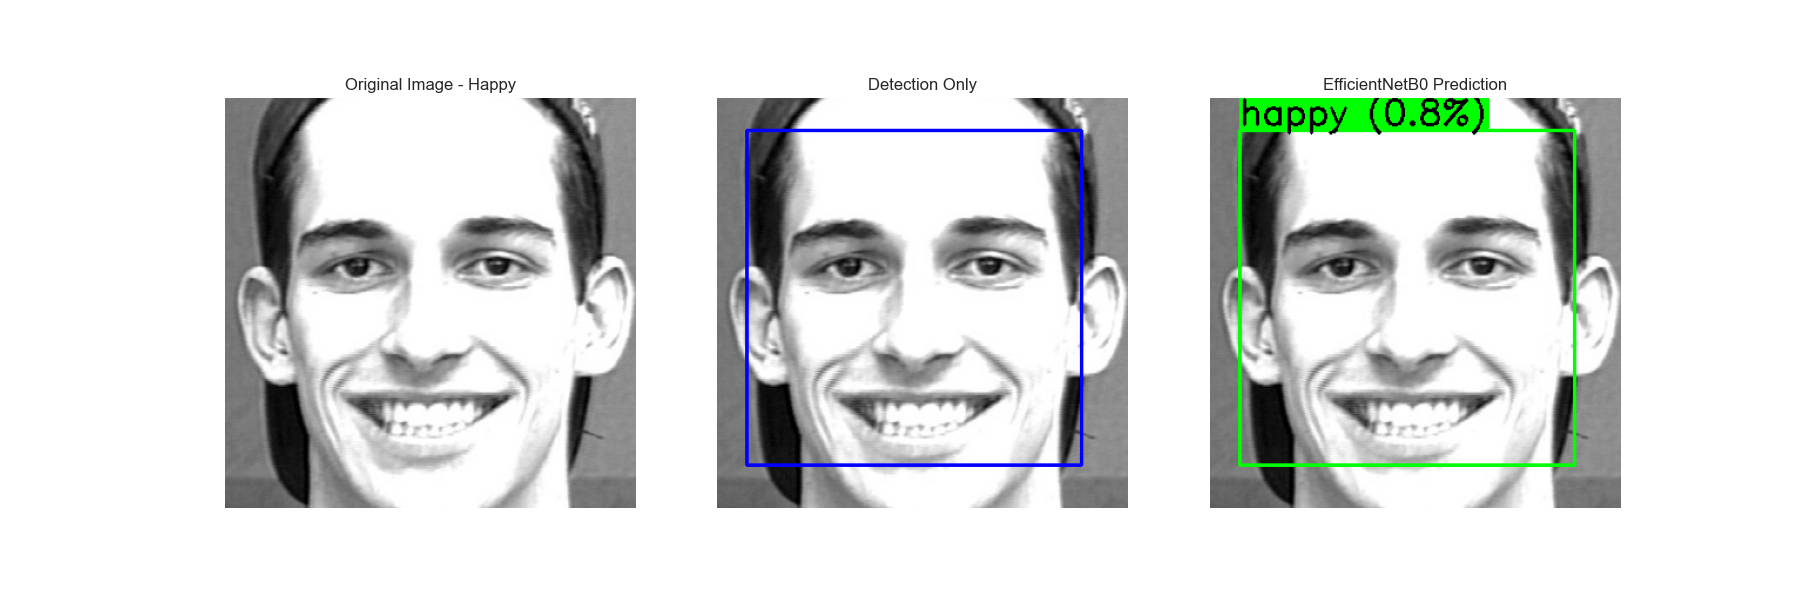
\includegraphics[width=1\textwidth]{figures/EfficientNetB0_Happy.png}
	\caption{Prediction - EfficientNet-B0 - Emotion: "Happy", Predicted: "Neutral"}
	\label{fig:predictions_efficientnet_03}
\end{figure}

\begin{figure}[h]
	\centering
	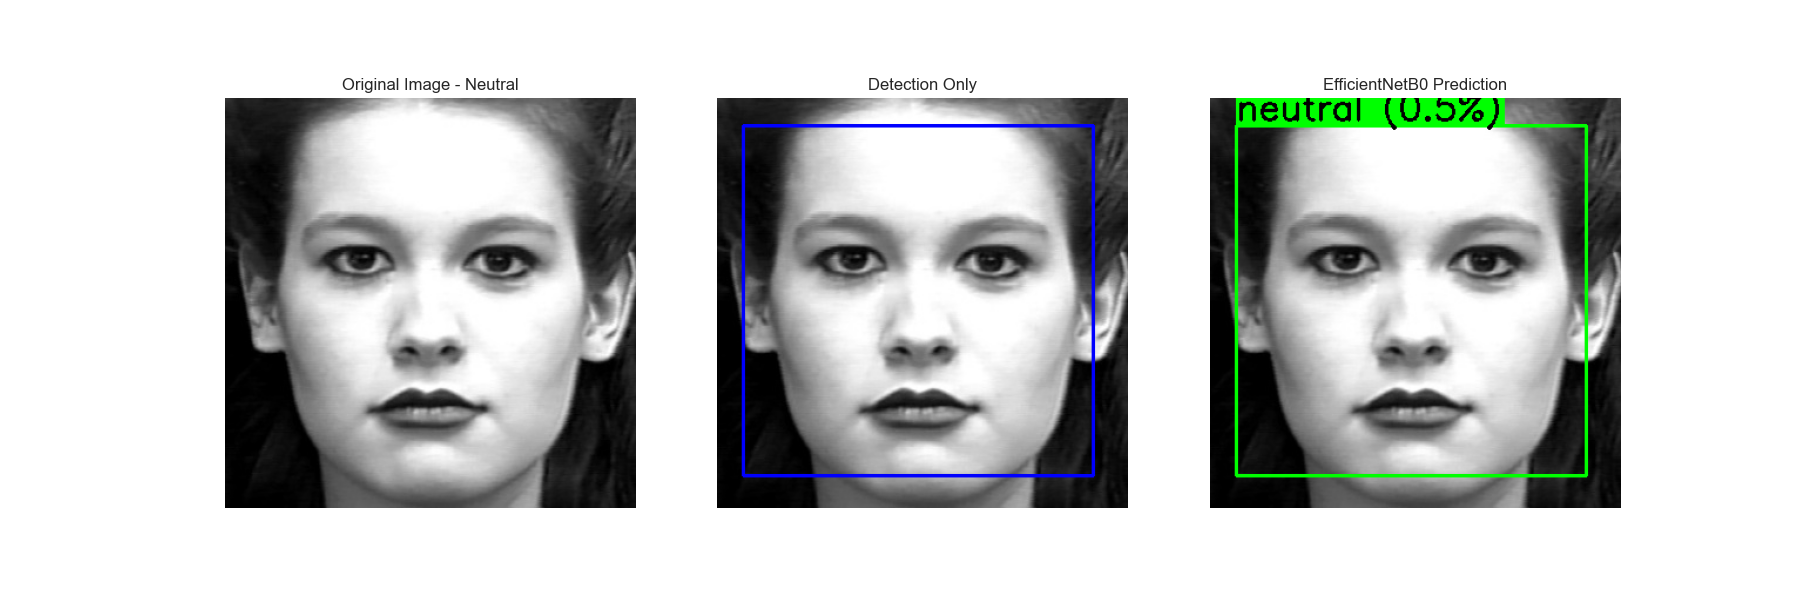
\includegraphics[width=1\textwidth]{figures/EfficientNetB0_Neutral.png}
	\caption{Prediction - EfficientNet-B0 - Emotion: "Neutral", Predicted: "Neutral"}
	\label{fig:predictions_efficientnet_04}
\end{figure}

\begin{figure}[h]
	\centering
	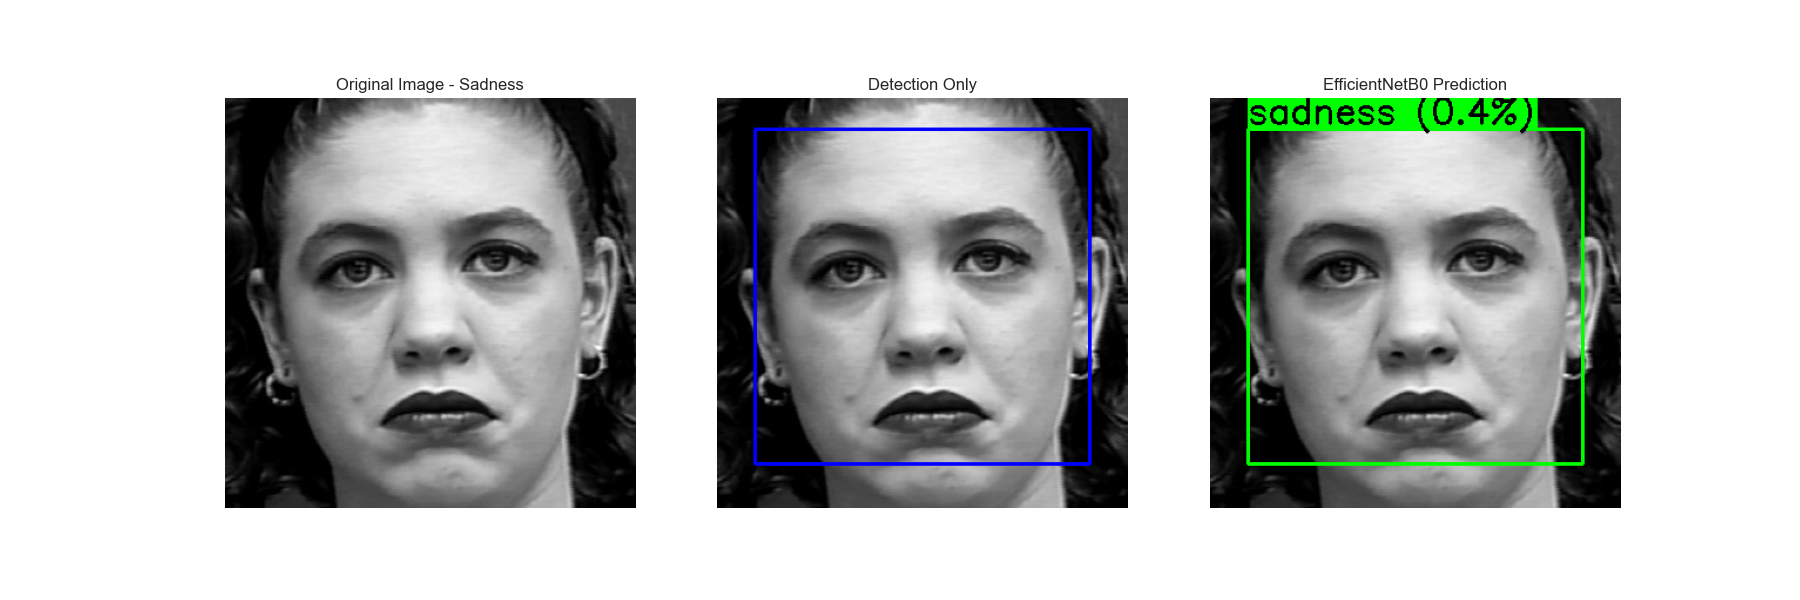
\includegraphics[width=1\textwidth]{figures/EfficientNetB0_Sadness.png}
	\caption{Prediction - EfficientNet-B0 - Emotion: "Sadness", Predicted: "Sadness"}
	\label{fig:predictions_efficientnet_05}
\end{figure}

\begin{figure}[h]
	\centering
	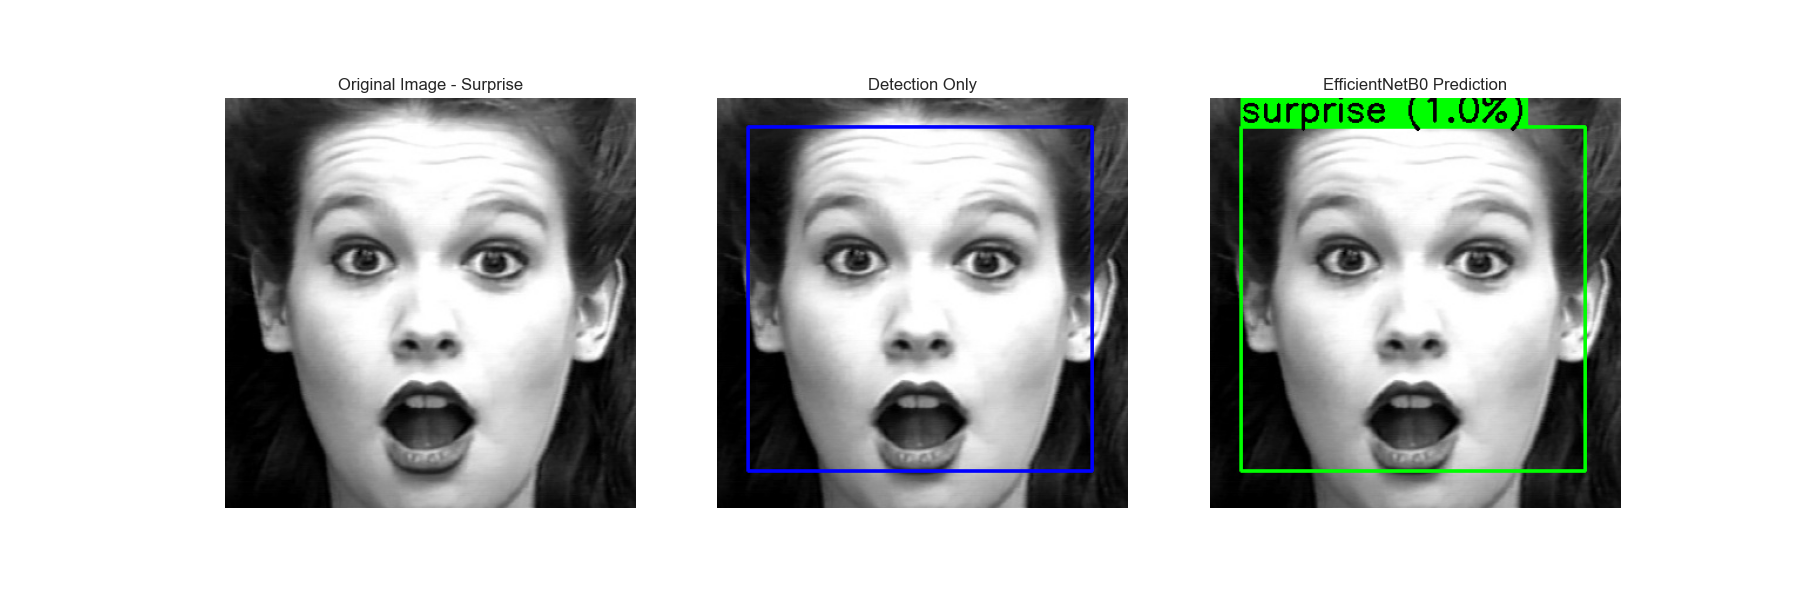
\includegraphics[width=1\textwidth]{figures/EfficientNetB0_Surprise.png}
	\caption{Prediction - EfficientNet-B0 - Emotion: "Surprise", Predicted: "Surprise"}
	\label{fig:predictions_efficientnet_06}
\end{figure}

\begin{figure}[h]
	\centering
	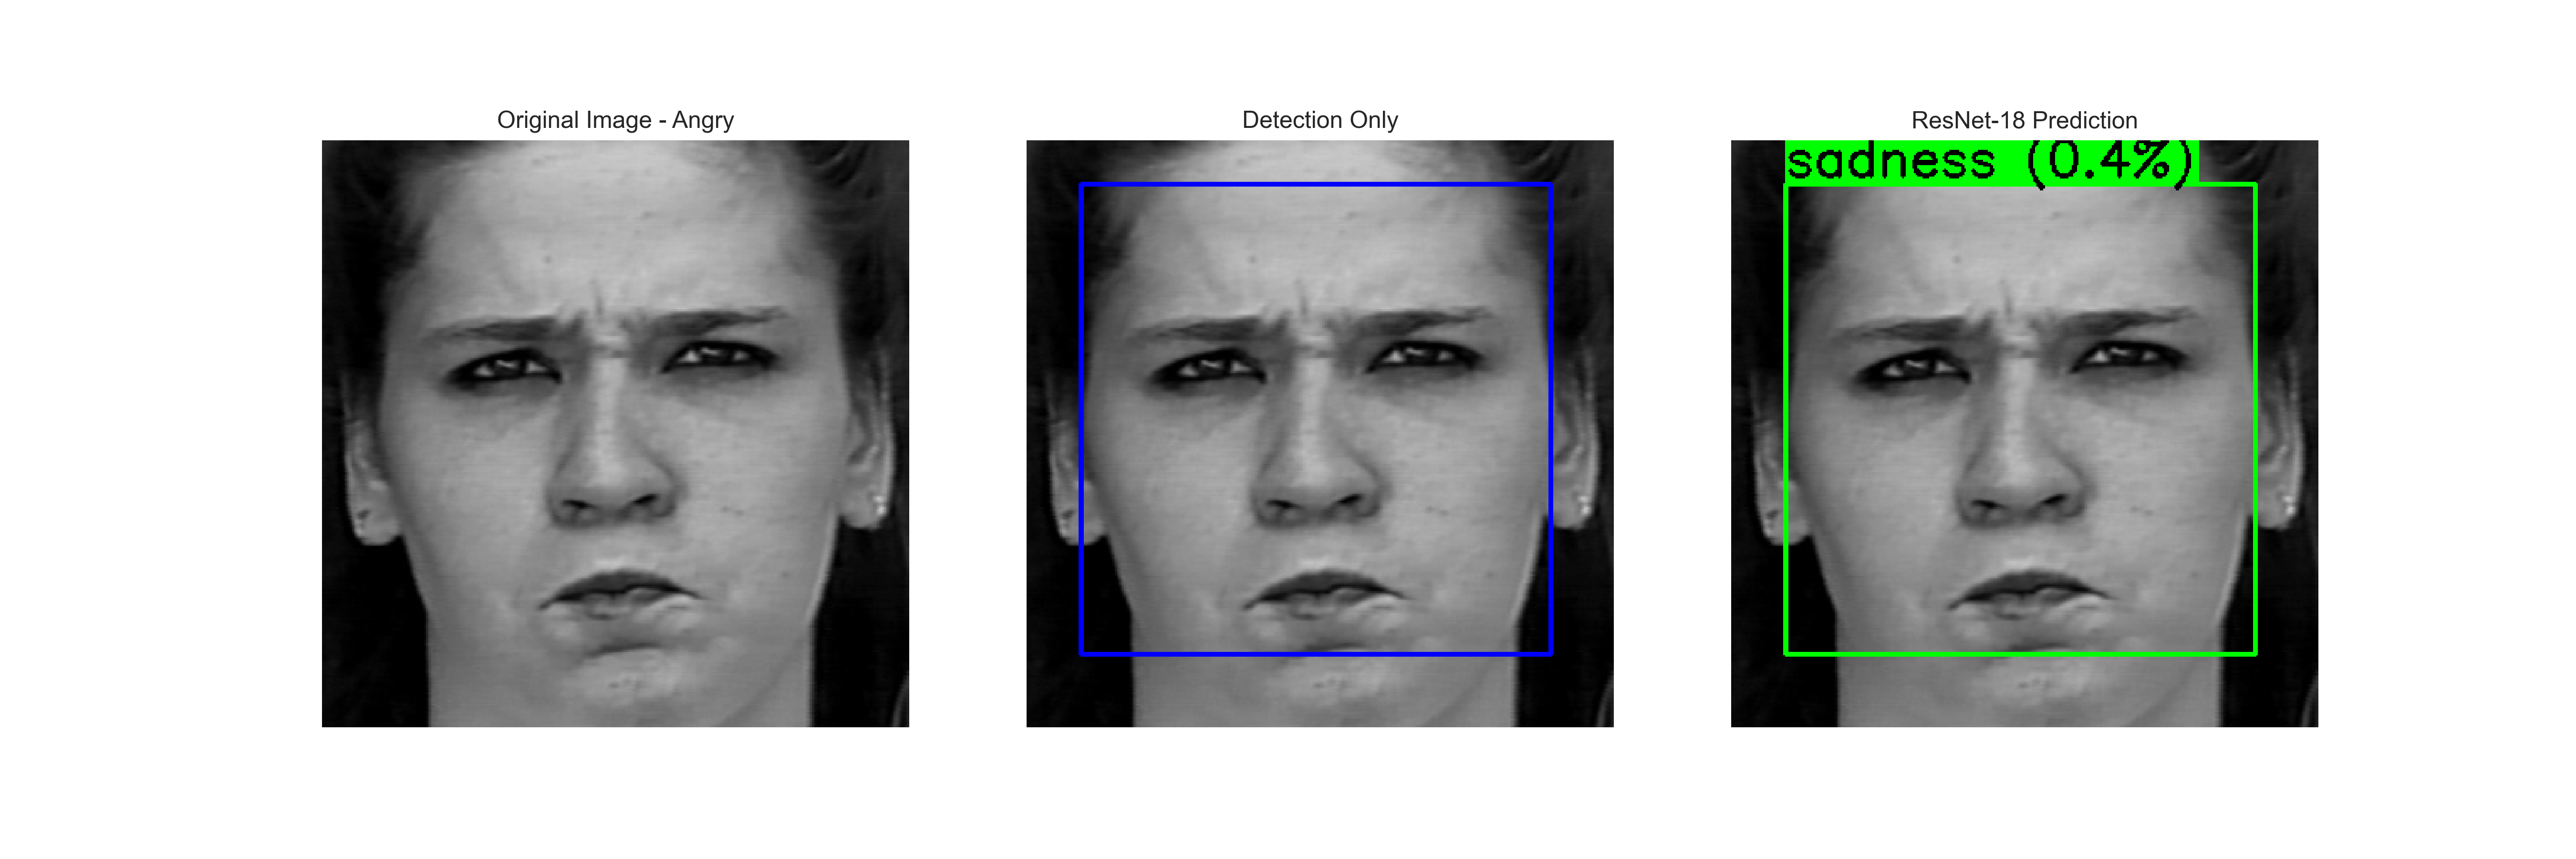
\includegraphics[width=1\textwidth]{figures/ResNet18_Angry.png}
	\caption{Prediction - ResNet18 - Emotion: "Angry", Predicted: "Sadness"}
	\label{fig:predictions_resnet_01}
\end{figure}

\begin{figure}[h]
	\centering
	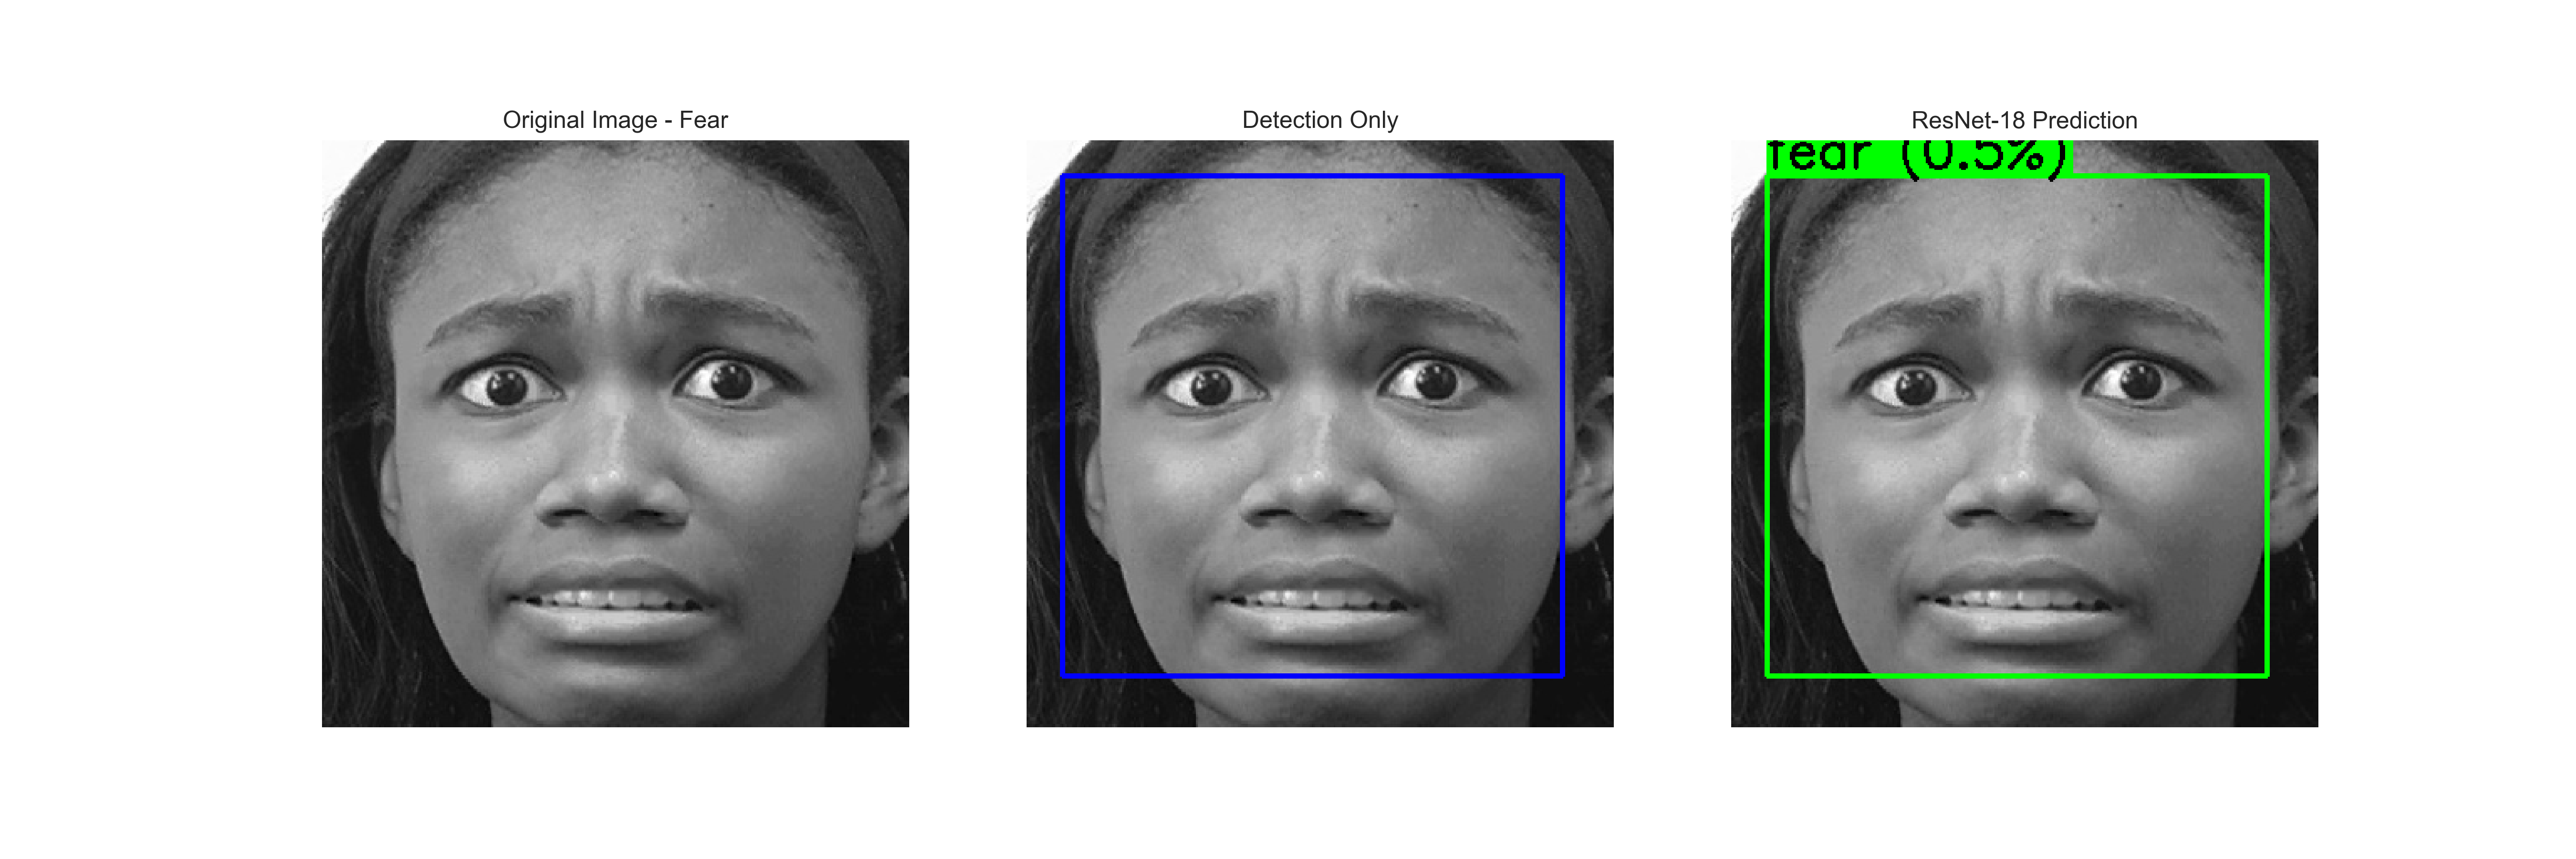
\includegraphics[width=1\textwidth]{figures/ResNet18_Fear.png}
	\caption{Prediction - ResNet18 - Emotion: "Fear", Predicted: "Fear"}
	\label{fig:predictions_resnet_02}
\end{figure}

\begin{figure}[h]
	\centering
	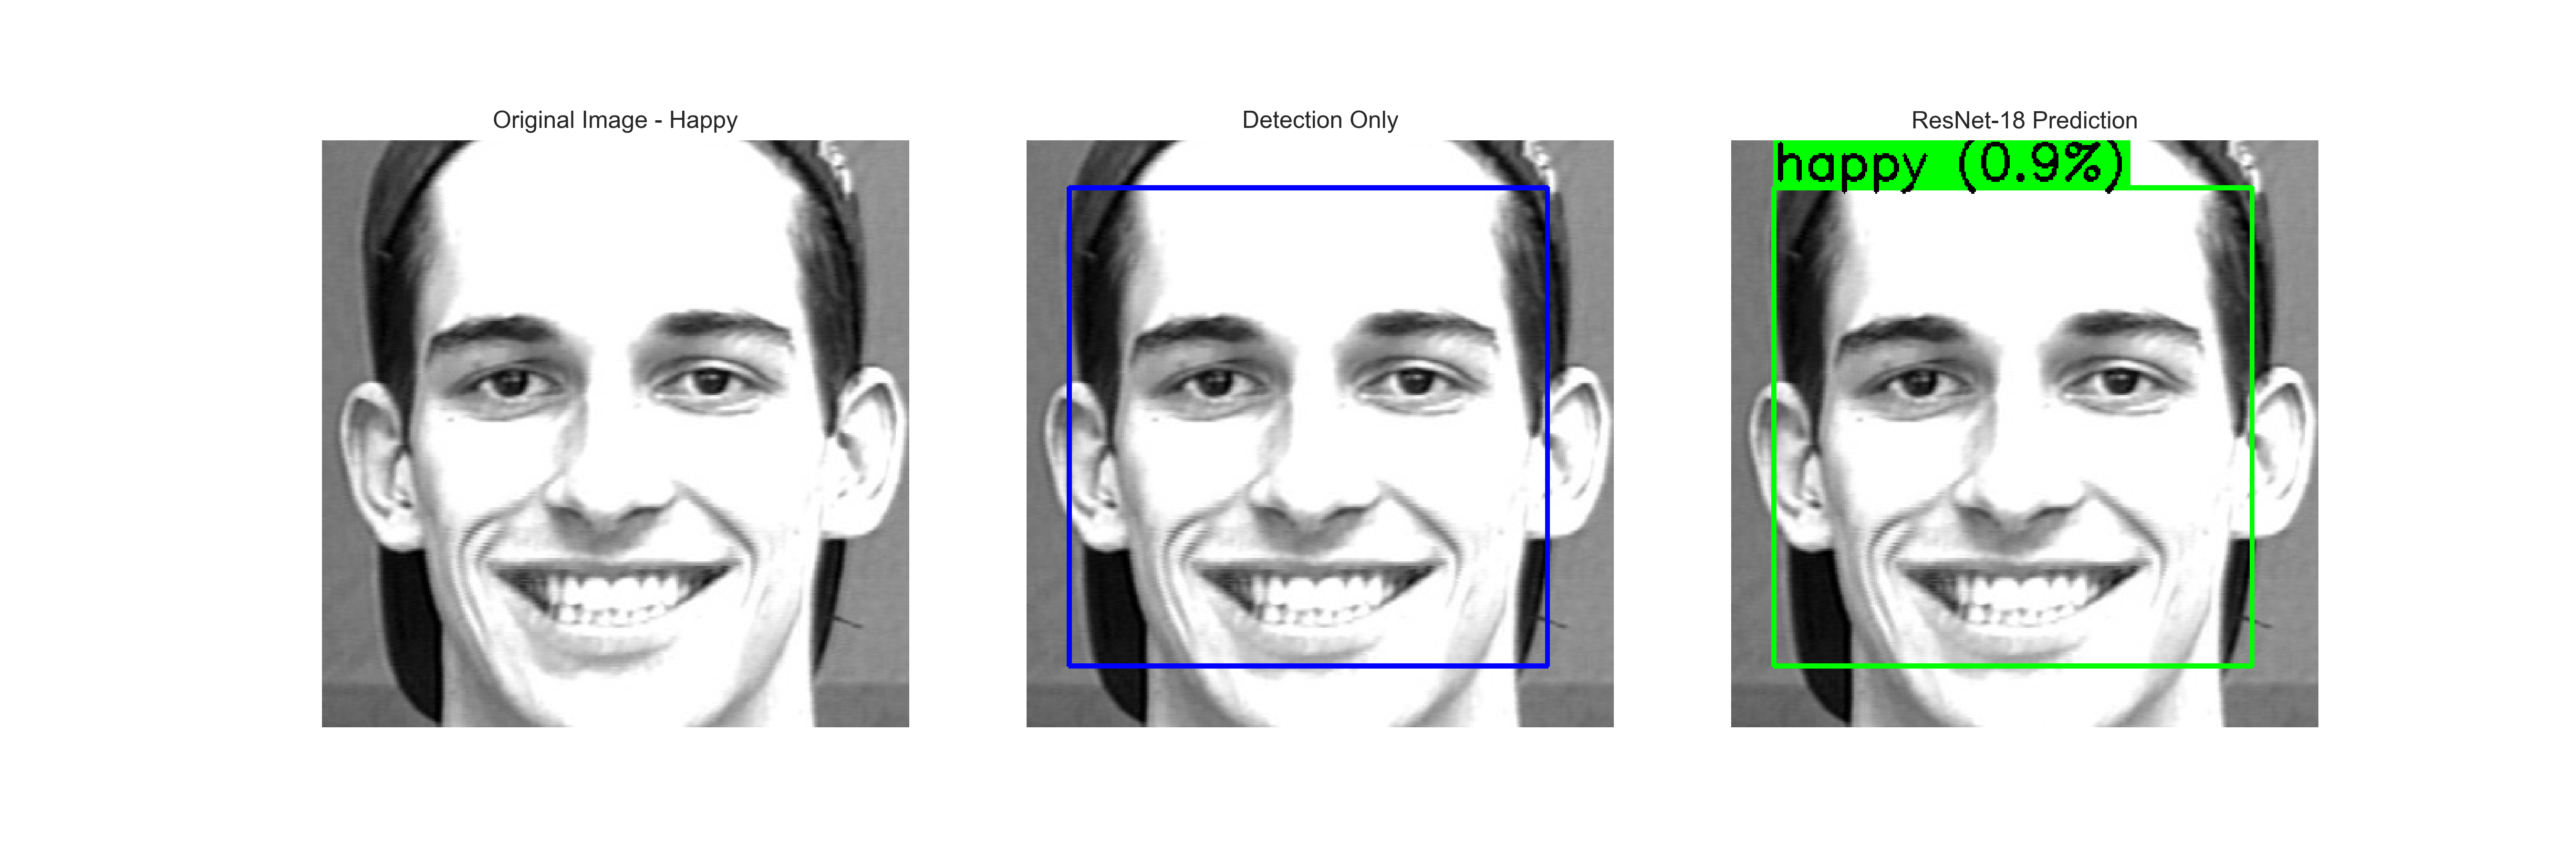
\includegraphics[width=1\textwidth]{figures/ResNet18_Happy.png}
	\caption{Prediction - ResNet18 - Emotion: "Happy", Predicted: "Happy"}
	\label{fig:predictions_resnet_03}
\end{figure}

\begin{figure}[h]
	\centering
	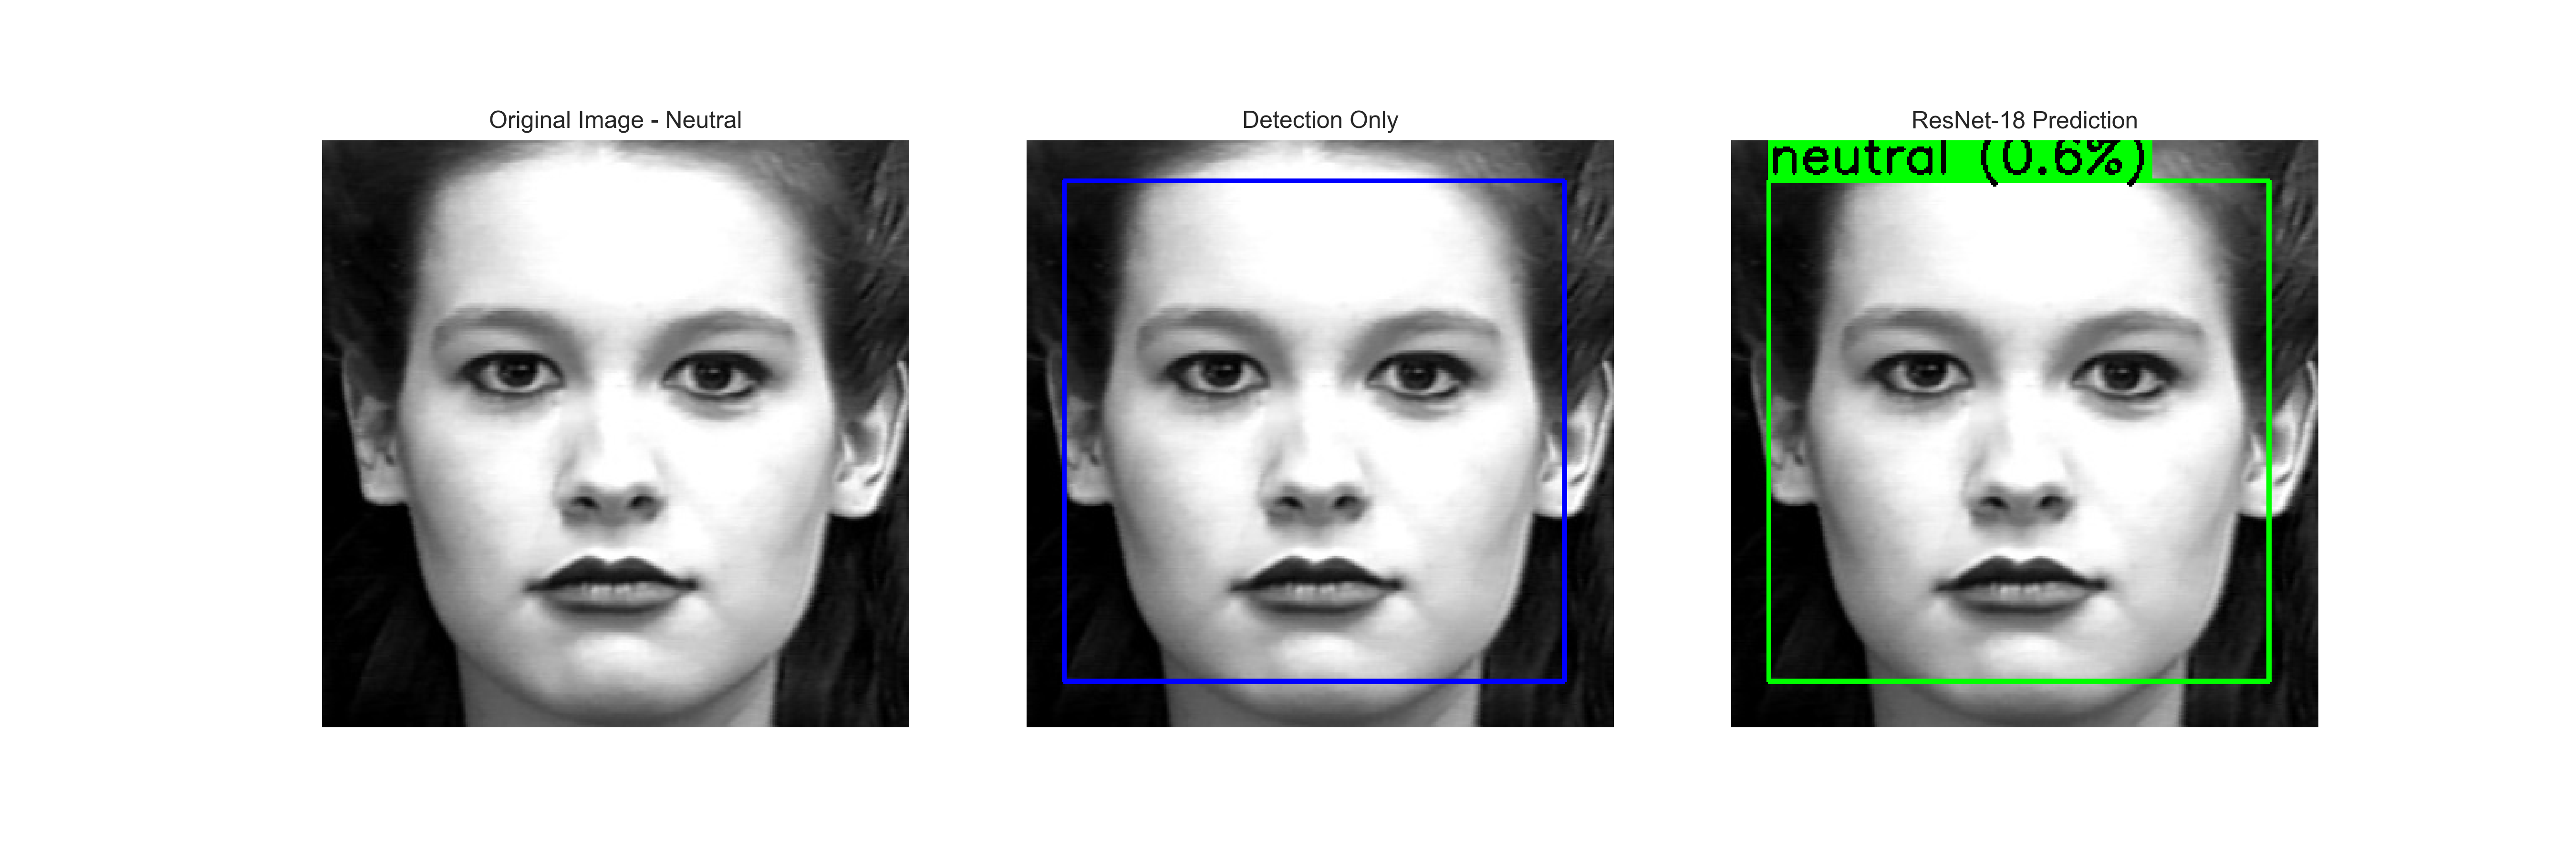
\includegraphics[width=1\textwidth]{figures/ResNet18_Neutral.png}
	\caption{Prediction - ResNet18 - Emotion: "Neutral", Predicted: "Neutral"}
	\label{fig:predictions_resnet_04}
\end{figure}

\begin{figure}[h]
	\centering
	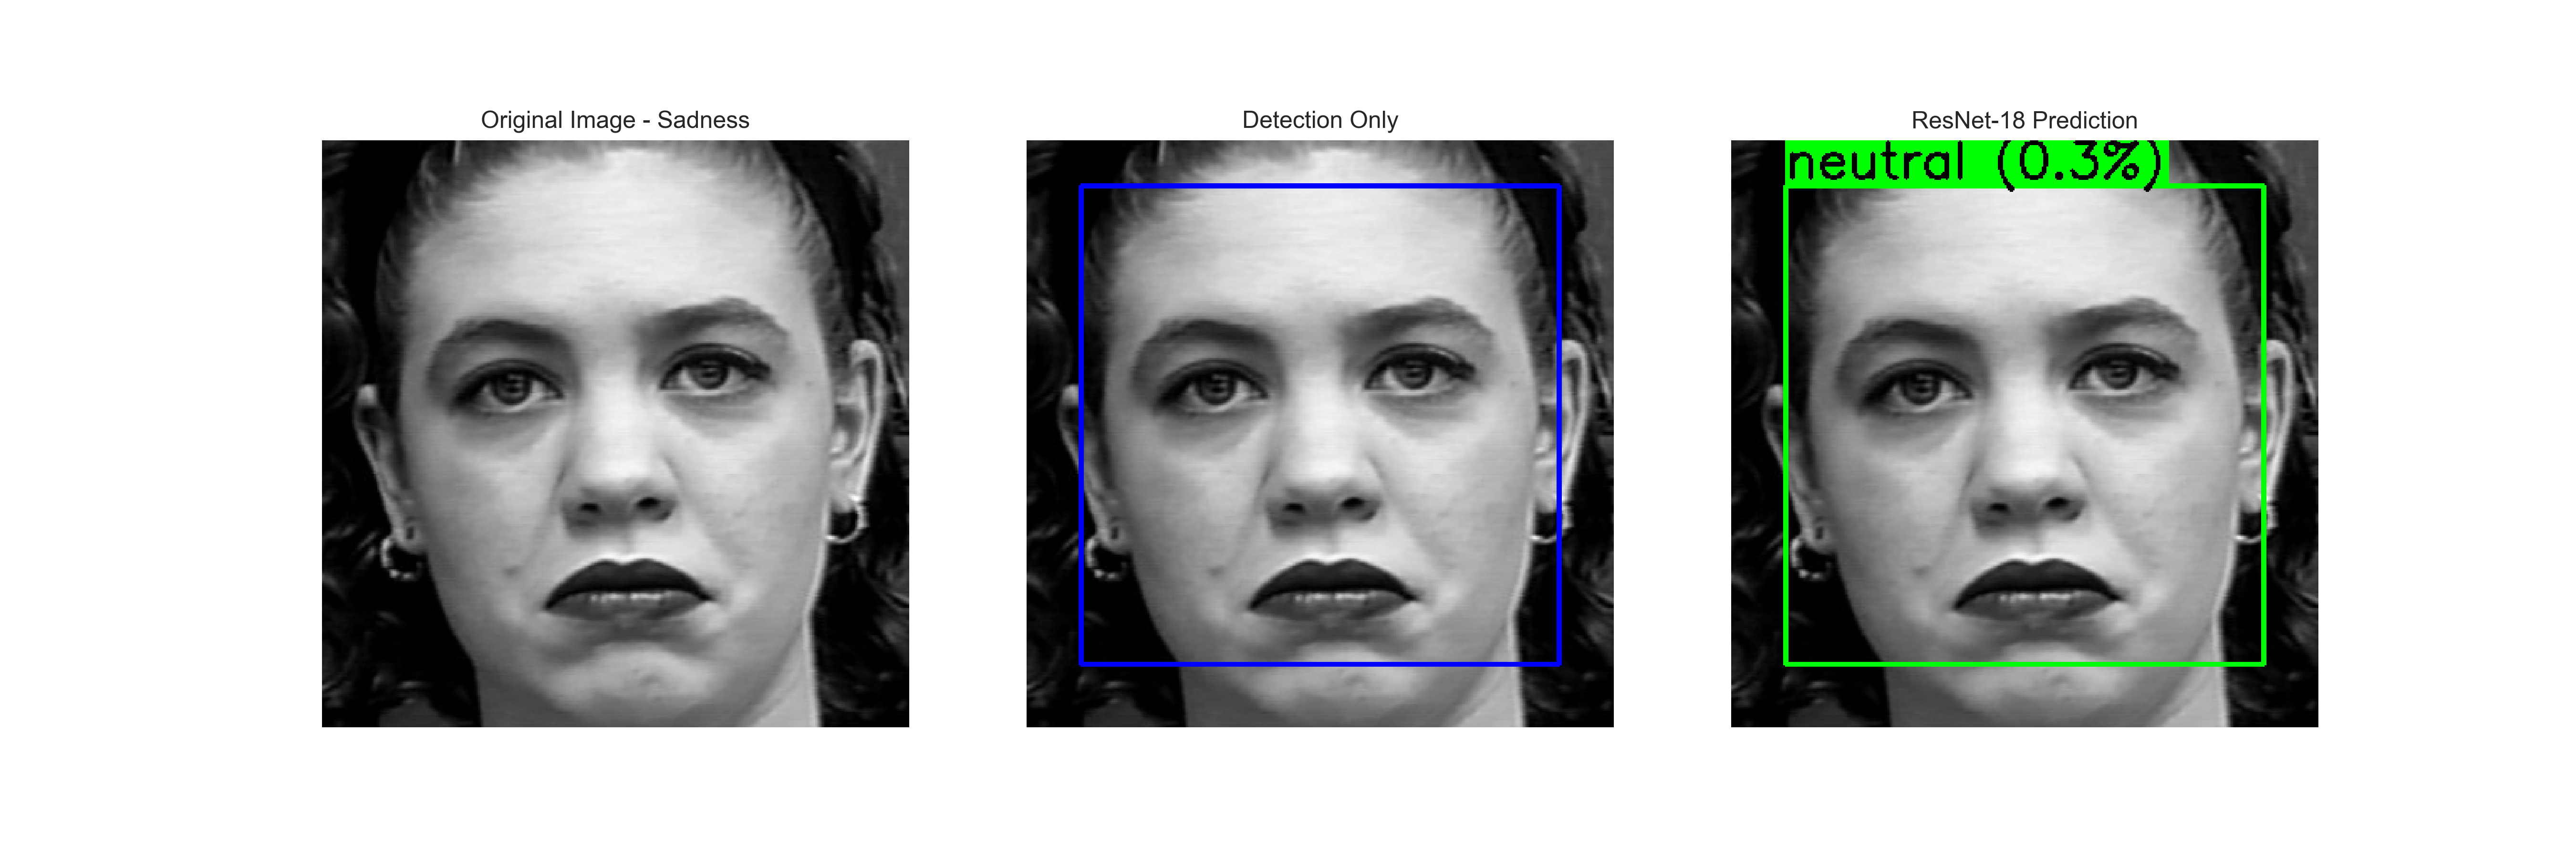
\includegraphics[width=1\textwidth]{figures/ResNet18_Sadness.png}
	\caption{Prediction - ResNet18 - Emotion: "Sadness", Predicted: "Neutral"}
	\label{fig:predictions_resnet_05}
\end{figure}

\begin{figure}[h]
	\centering
	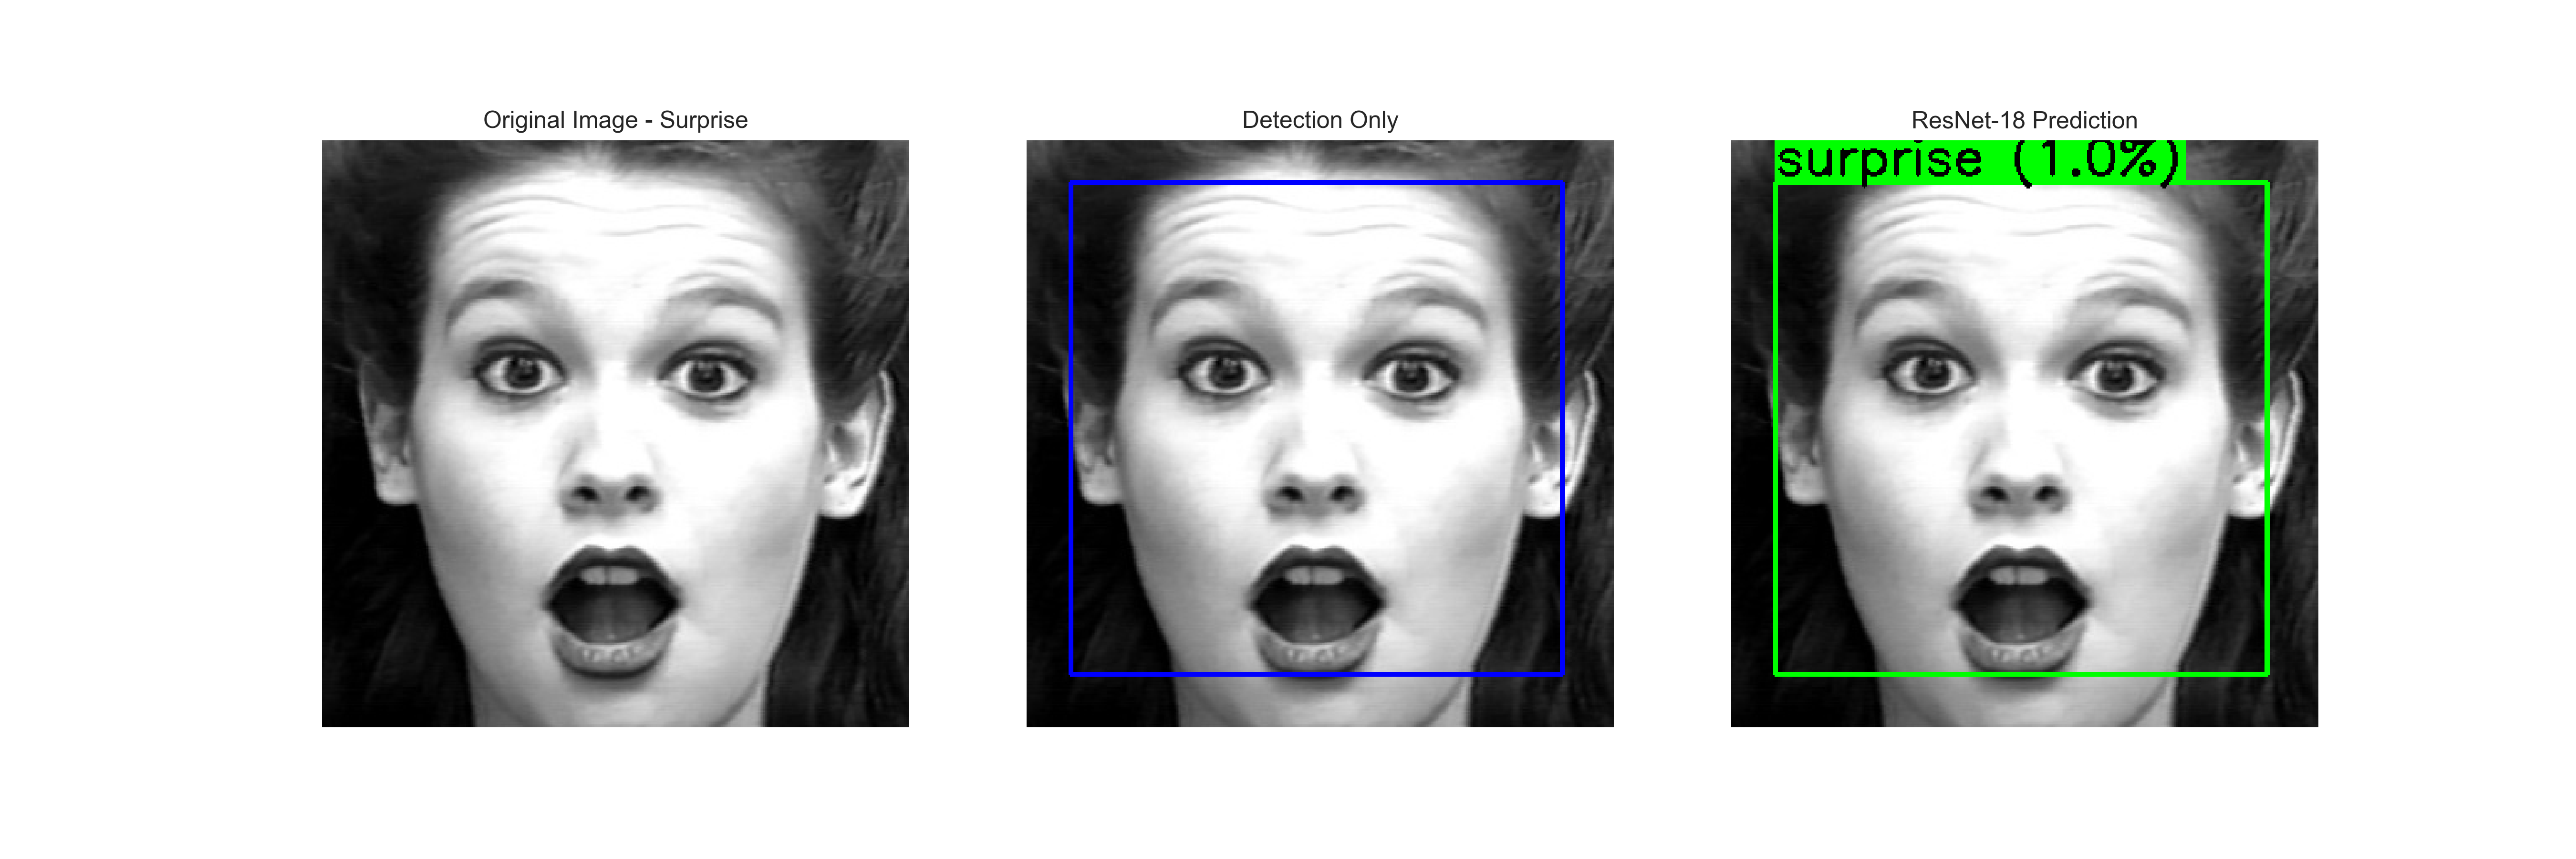
\includegraphics[width=1\textwidth]{figures/ResNet18_Surprise.png}
	\caption{Prediction - ResNet18 - Emotion: "Surprise", Predicted: "Surprise"}
	\label{fig:predictions_resnet_06}
\end{figure}

\begin{figure}[h]
	\centering
	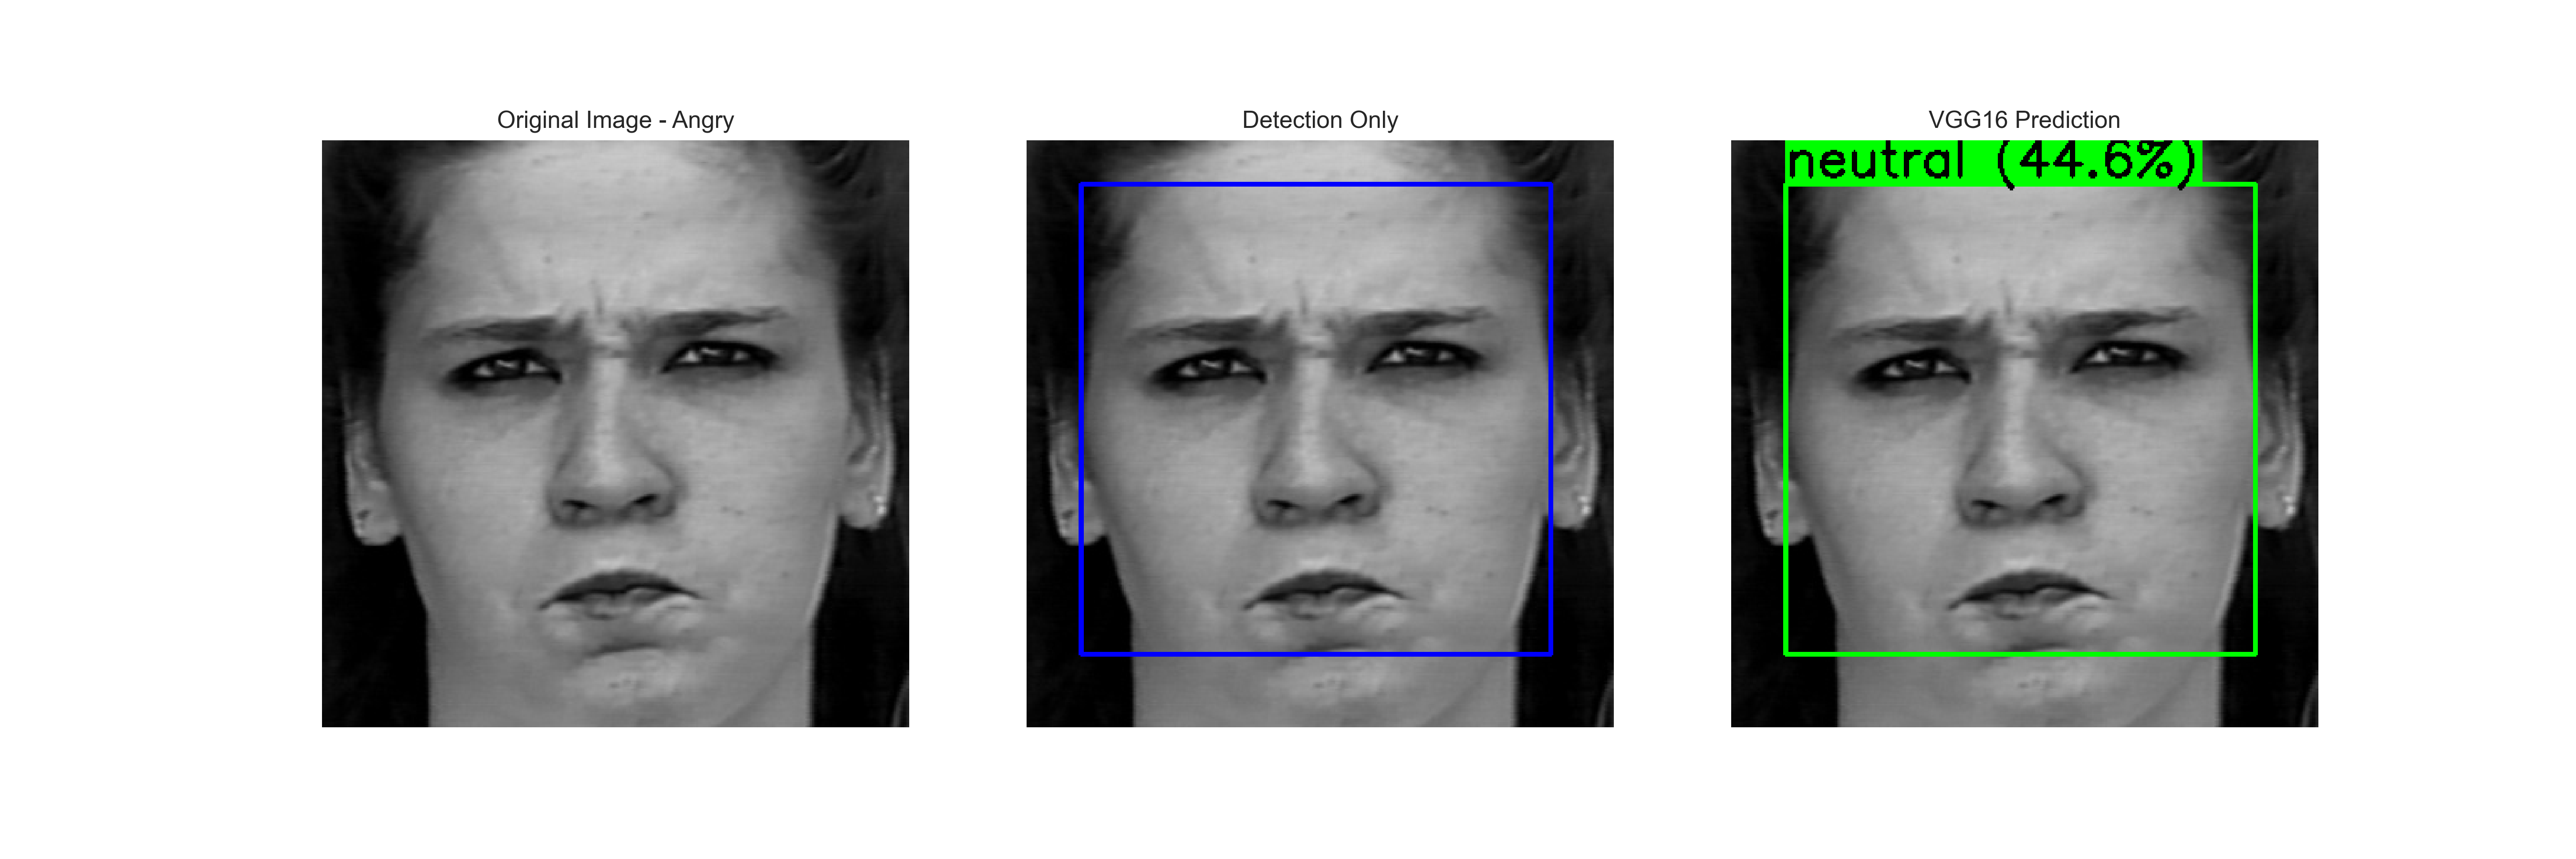
\includegraphics[width=1\textwidth]{figures/VGG16_Angry.png}
	\caption{Prediction - VGG16 - Emotion: "Angry", Predicted: "Neutral"}
	\label{fig:predictions_VGG16_01}
\end{figure}

\begin{figure}[h]
	\centering
	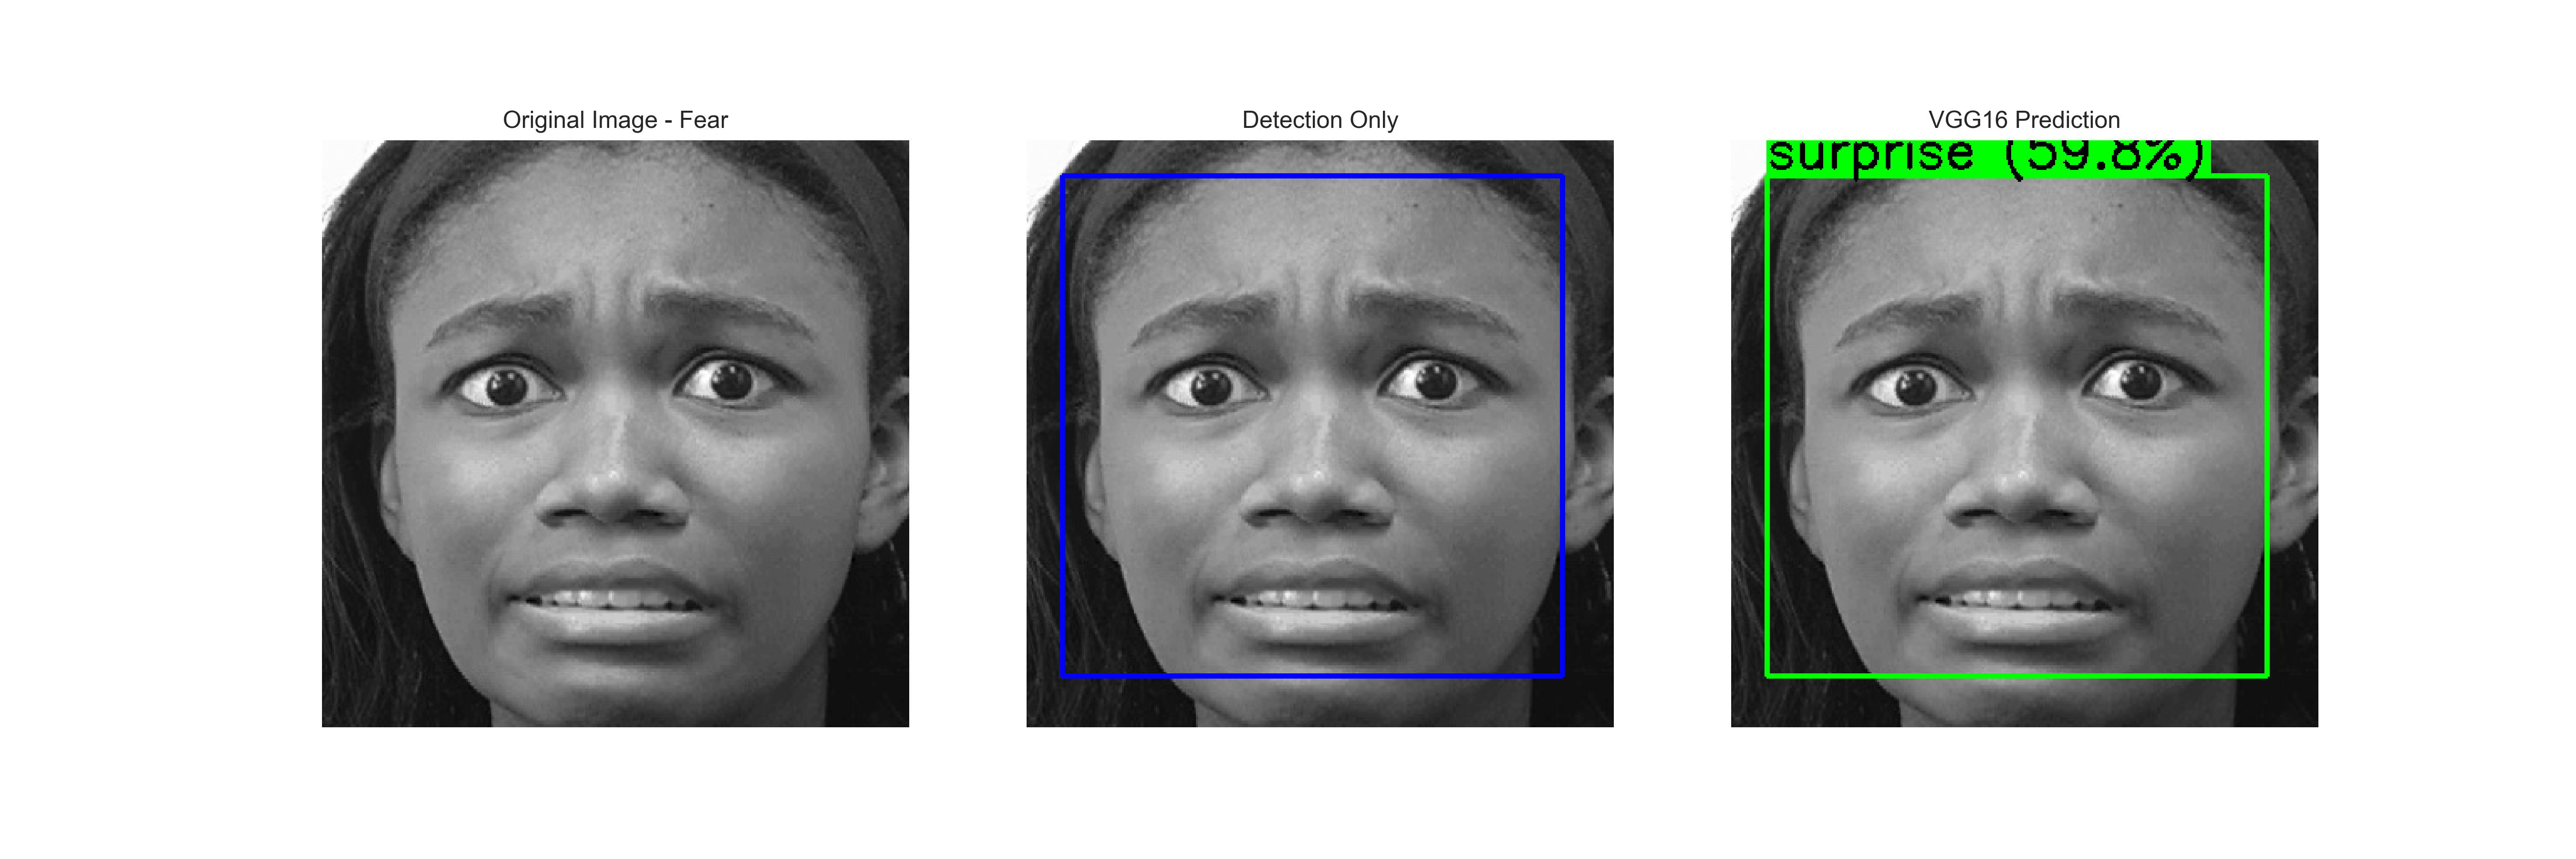
\includegraphics[width=1\textwidth]{figures/VGG16_Fear.png}
	\caption{Prediction - VGG16 - Emotion: "Fear", Predicted: "Surprise"}
	\label{fig:predictions_VGG16_02}
\end{figure}

\begin{figure}[h]
	\centering
	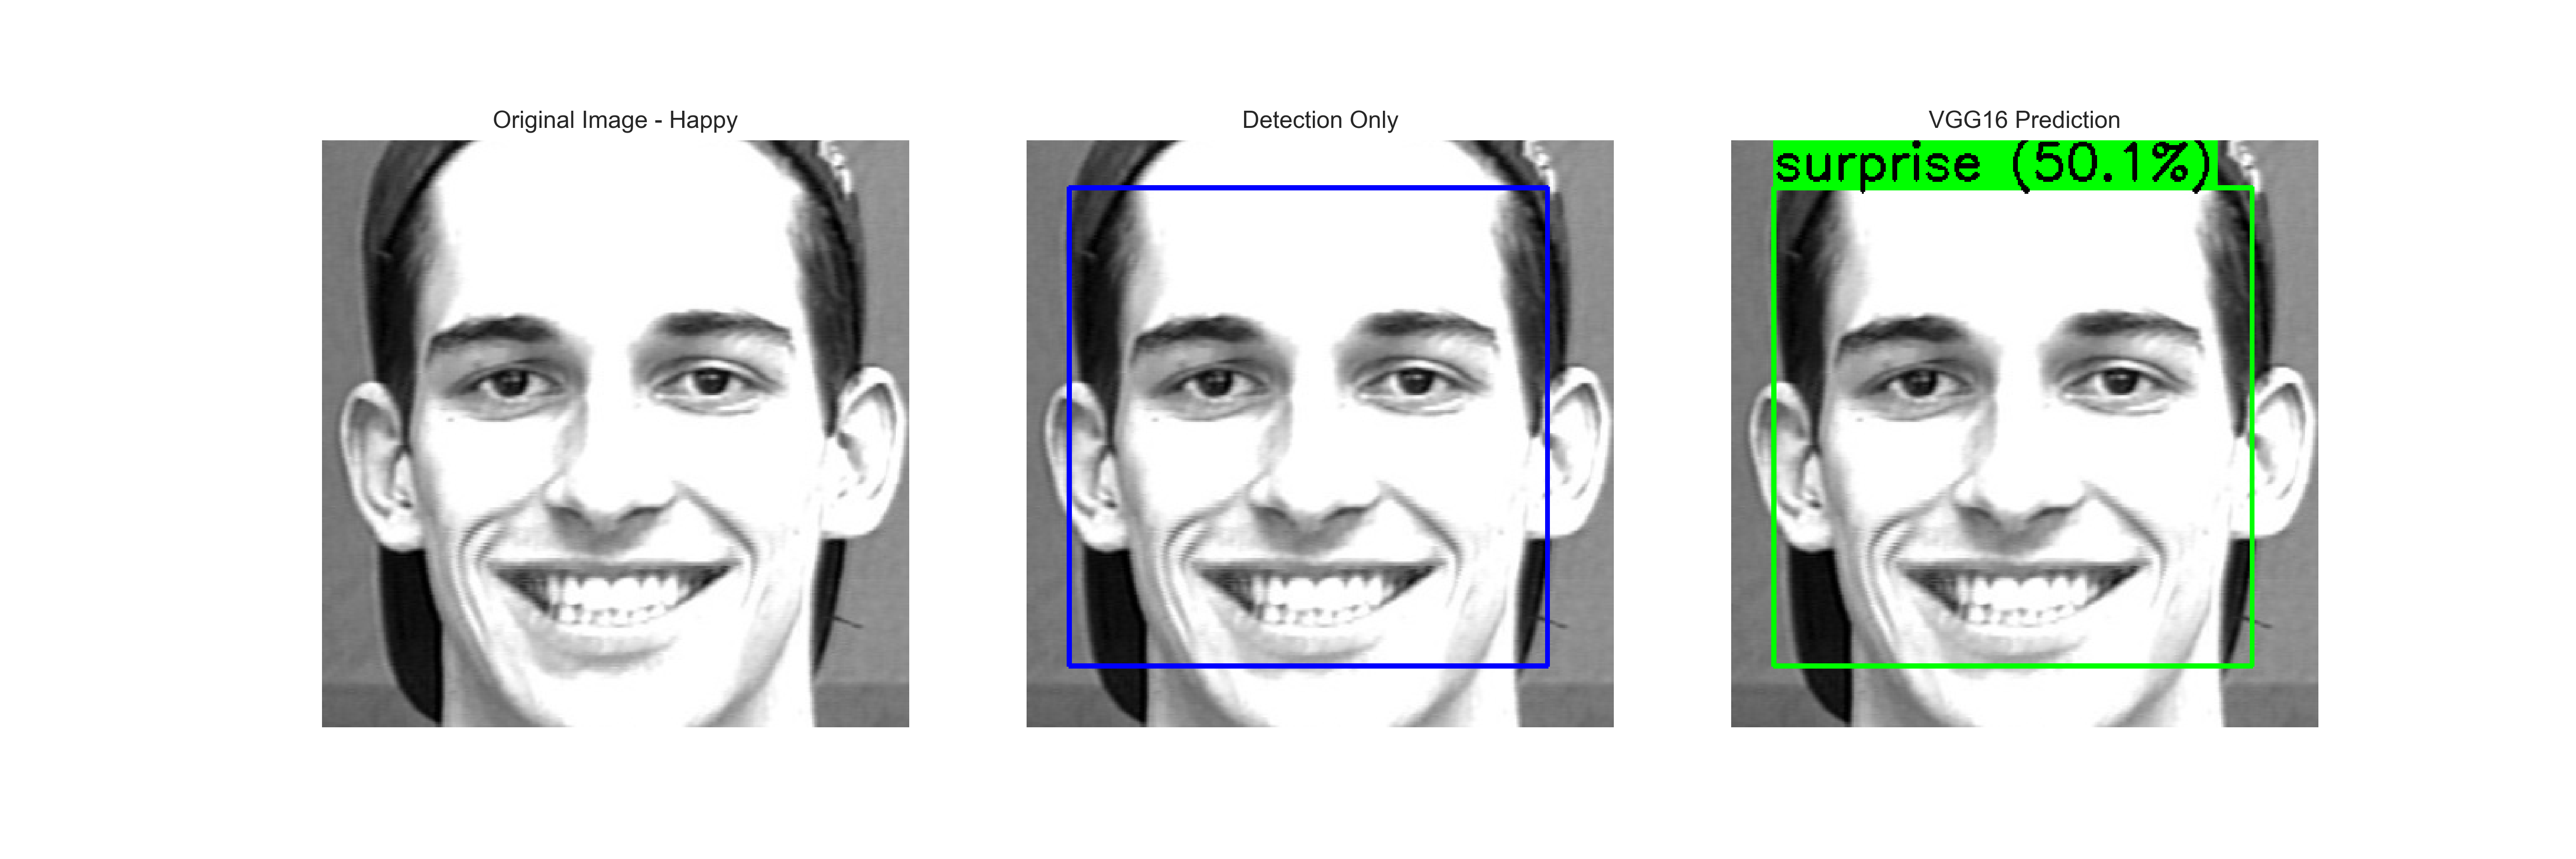
\includegraphics[width=1\textwidth]{figures/VGG16_Happy.png}
	\caption{Prediction - VGG16 - Emotion: "Happy", Predicted: "Surprise"}
	\label{fig:predictions_VGG16_03}
\end{figure}

\begin{figure}[h]
	\centering
	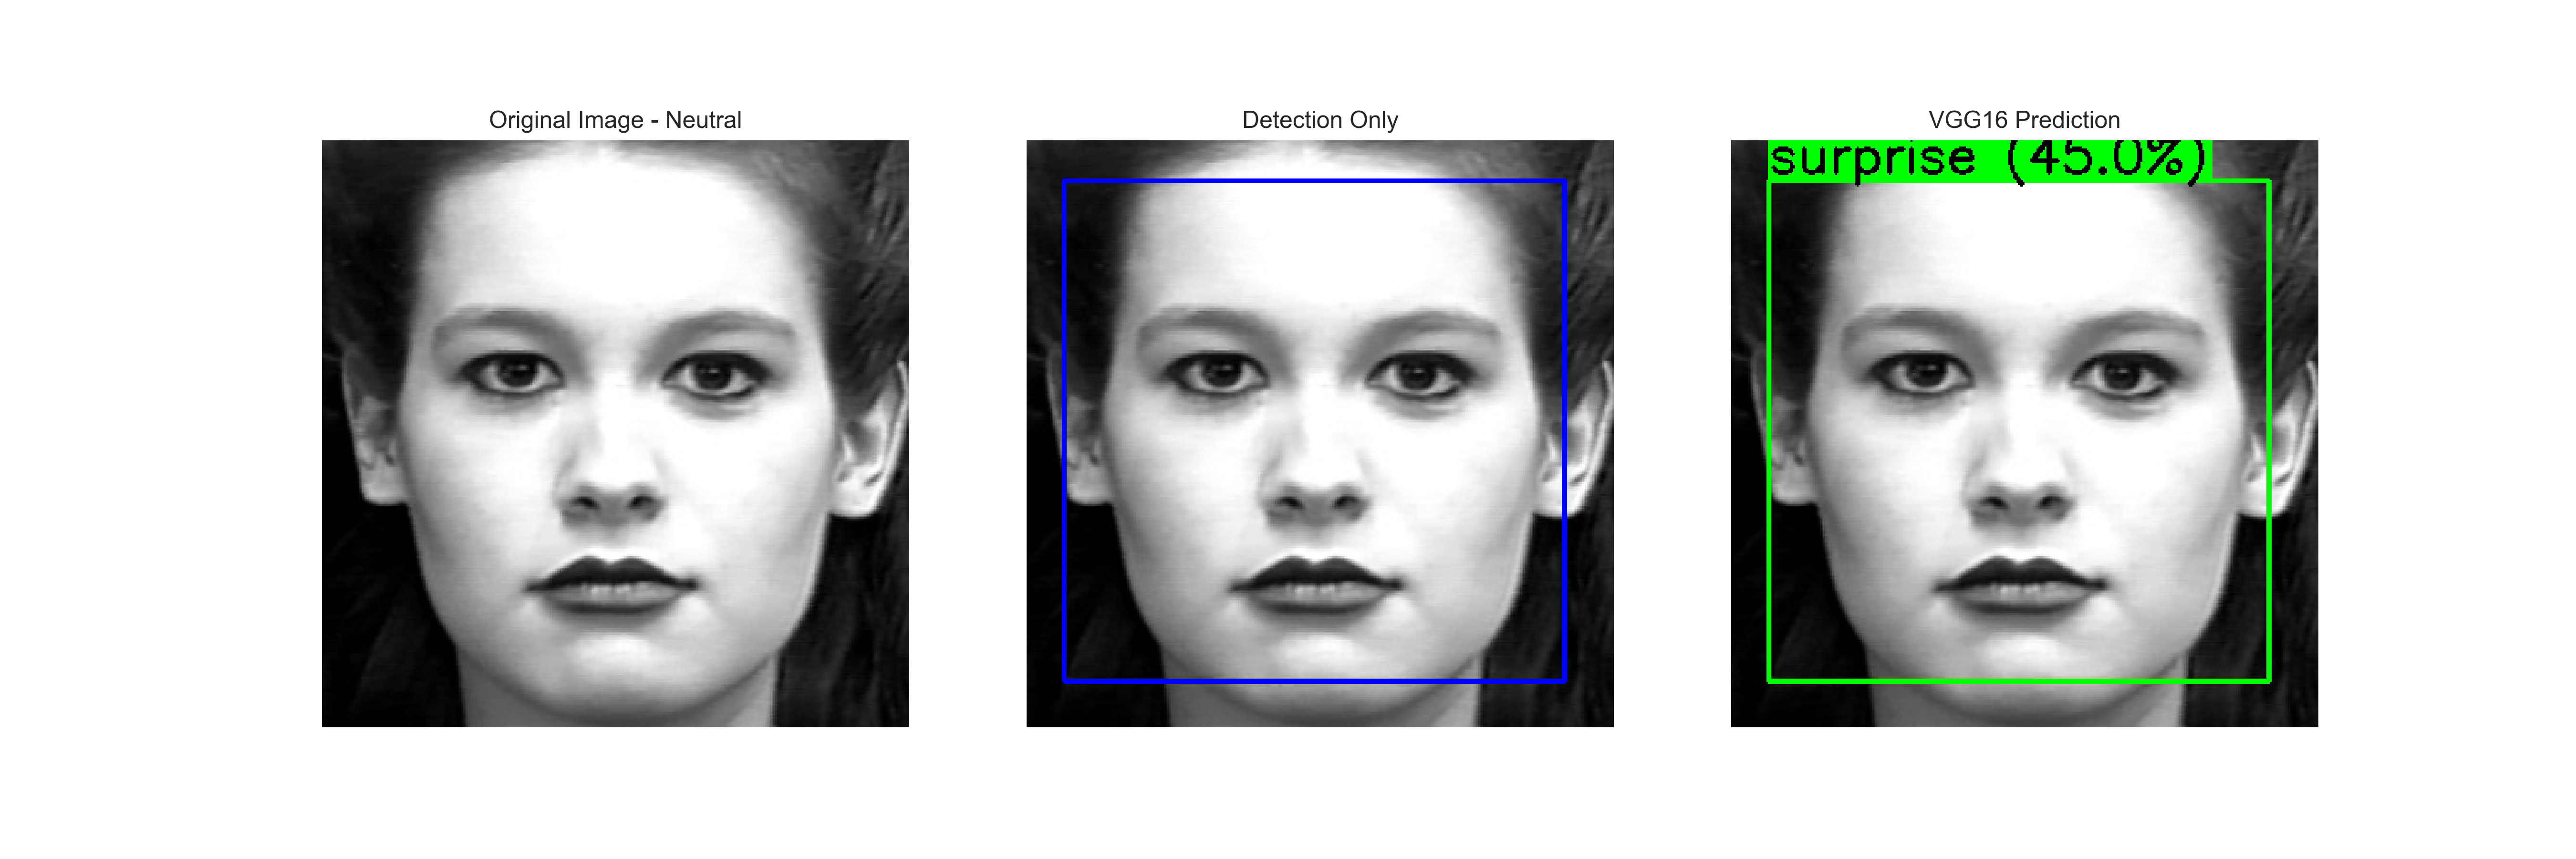
\includegraphics[width=1\textwidth]{figures/VGG16_Neutral.png}
	\caption{Prediction - VGG16 - Emotion: "Neutral", Predicted: "Surprise"}
	\label{fig:predictions_VGG16_04}
\end{figure}

\begin{figure}[h]
	\centering
	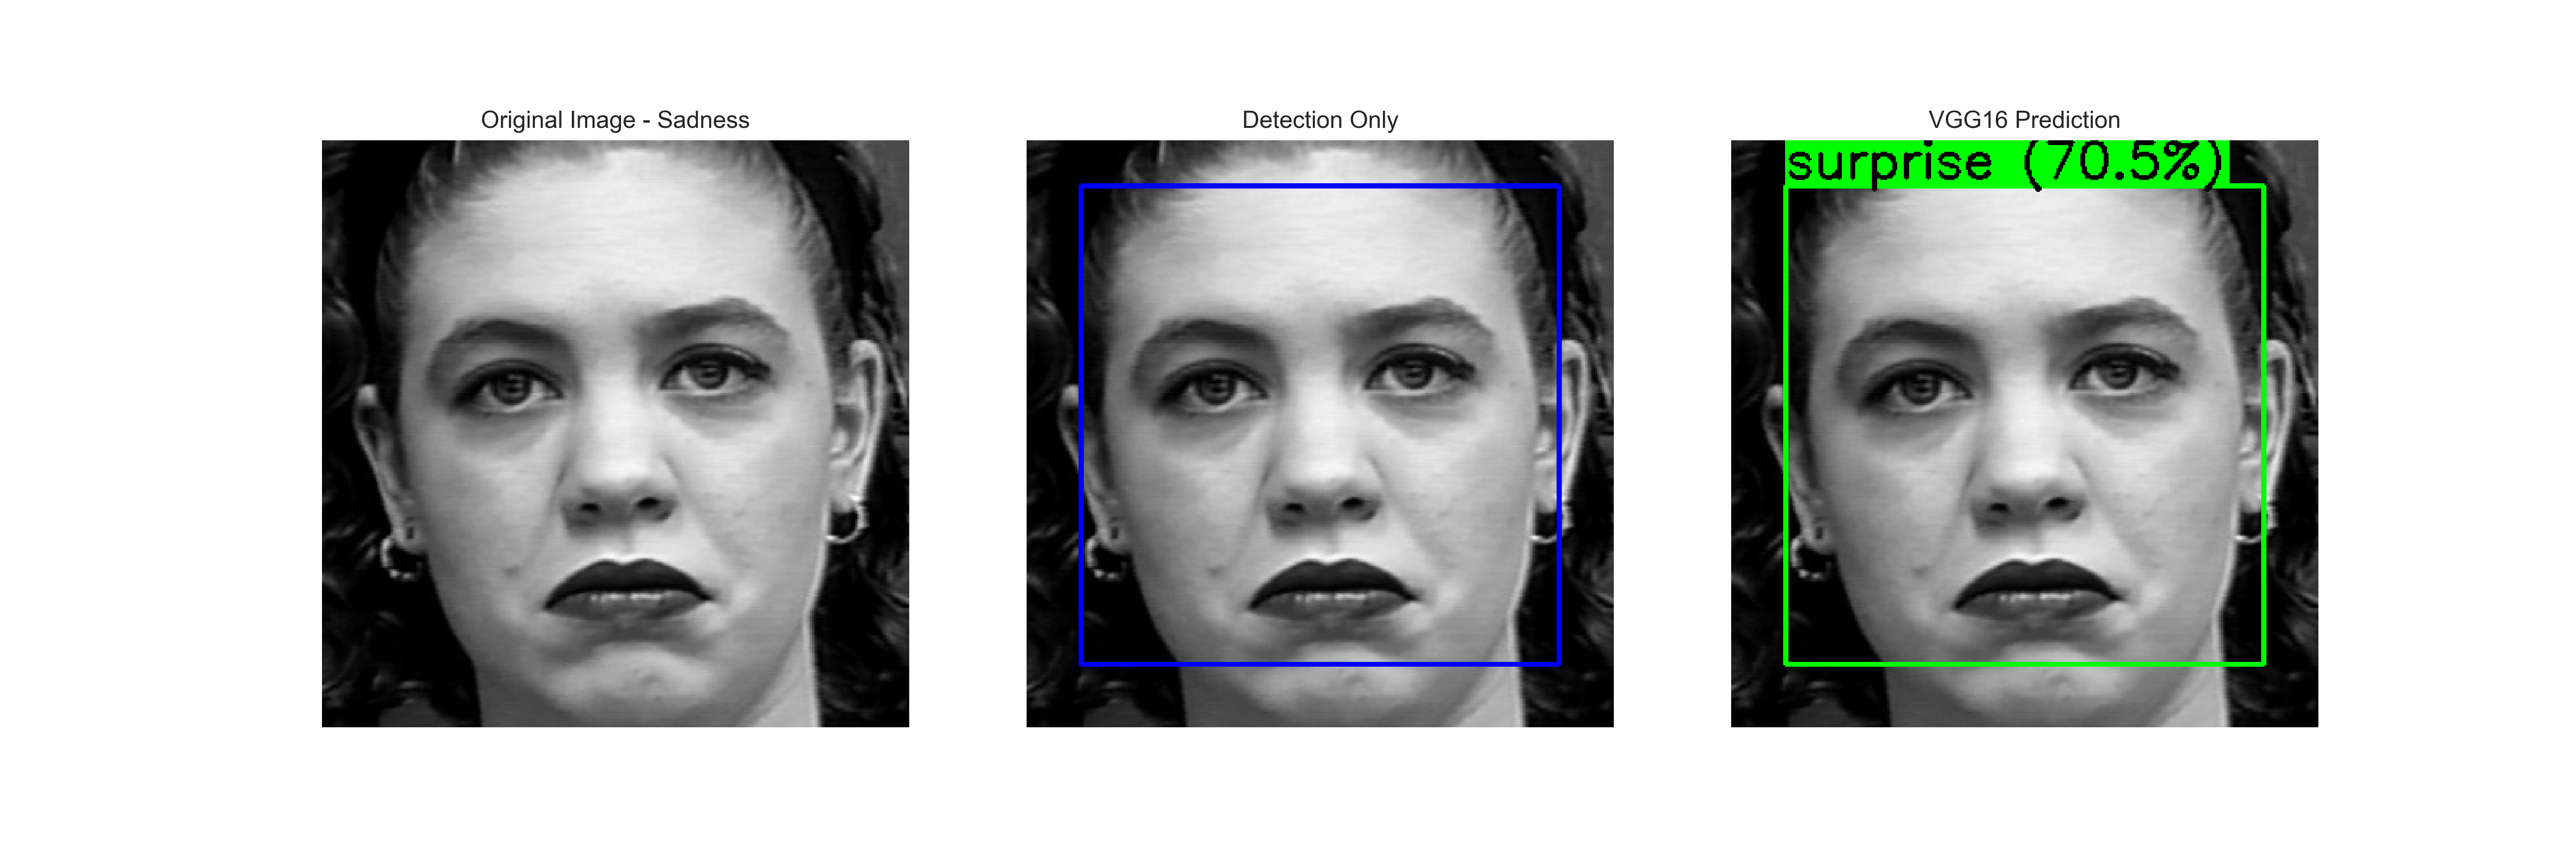
\includegraphics[width=1\textwidth]{figures/VGG16_Sadness.png}
	\caption{Prediction - VGG16 - Emotion: "Sadness", Predicted: "Surprise"}
	\label{fig:predictions_VGG16_05}
\end{figure}

\begin{figure}[h]
	\centering
	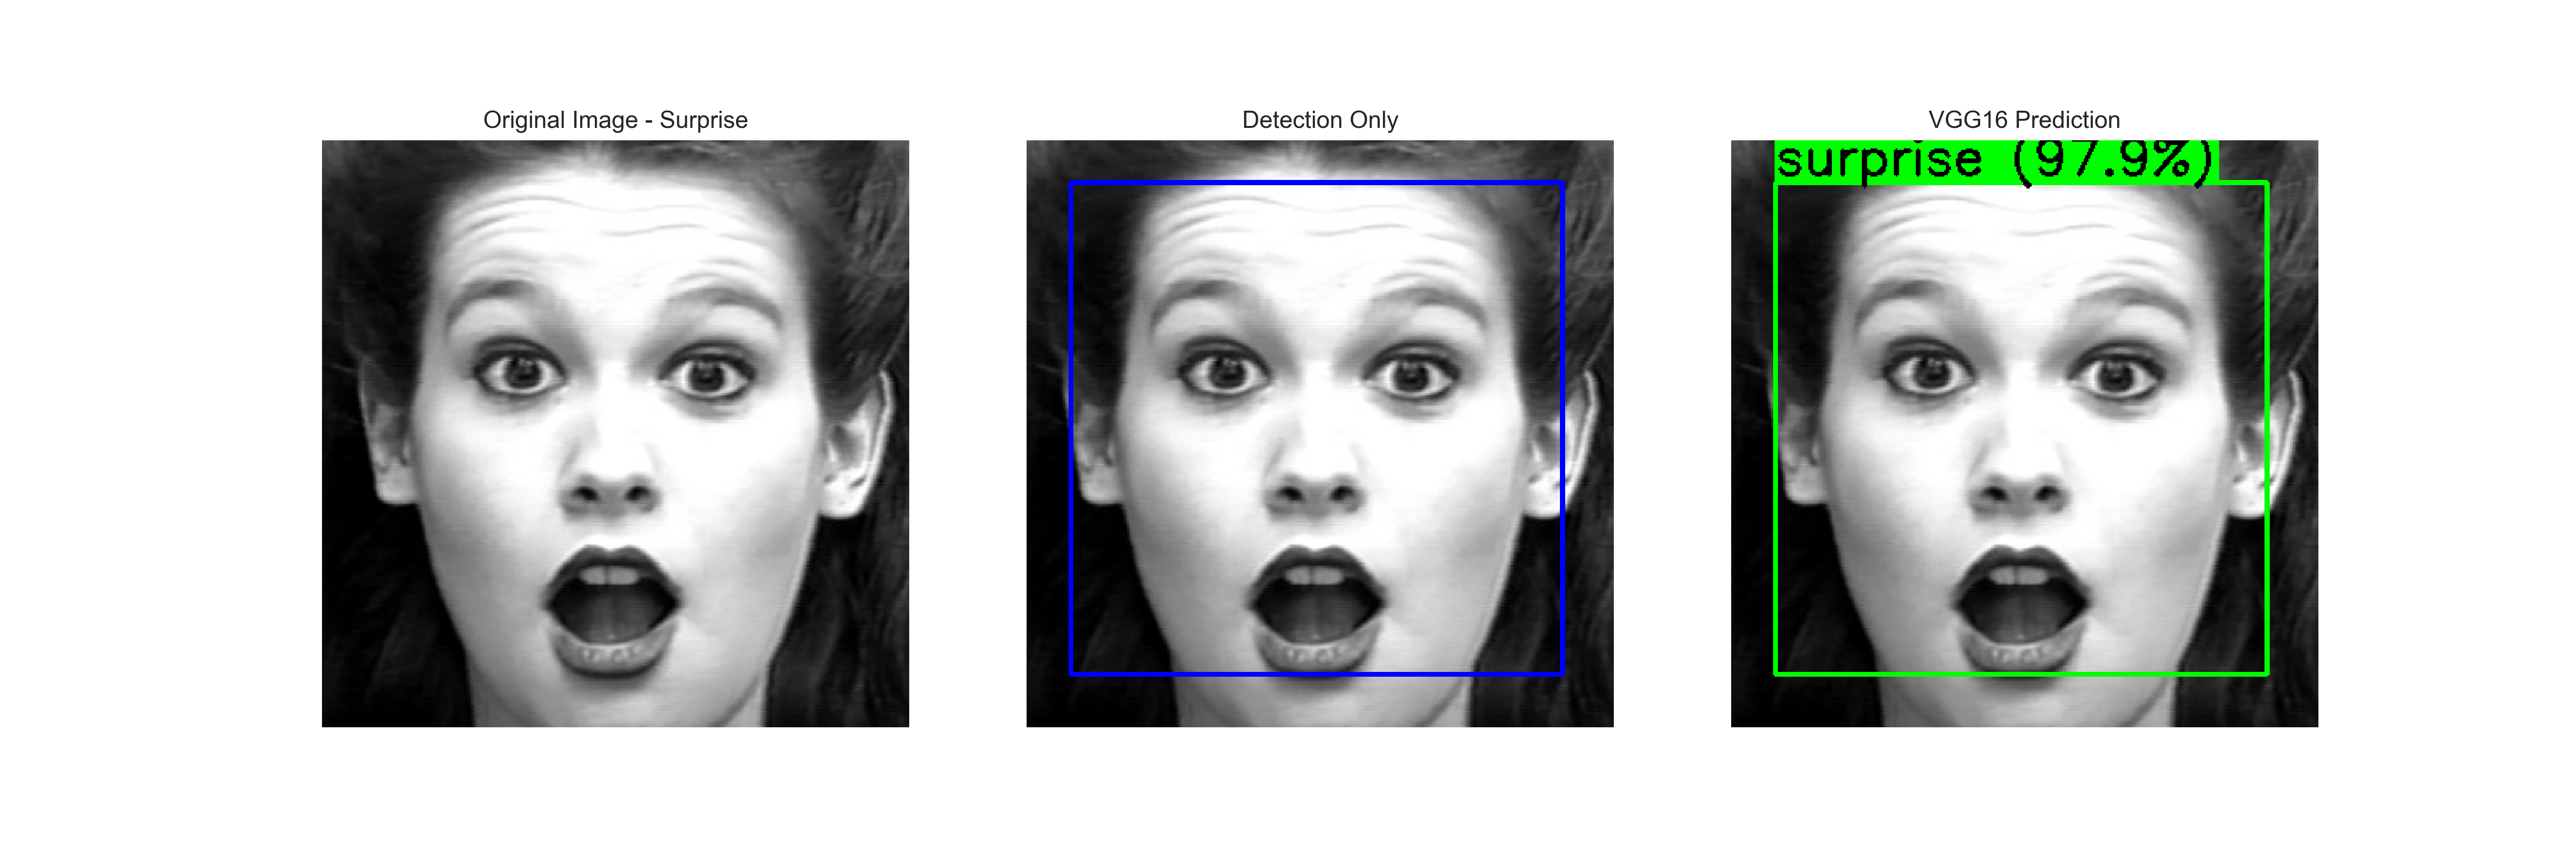
\includegraphics[width=1\textwidth]{figures/VGG16_Surprise.png}
	\caption{Prediction - VGG16 - Emotion: "Surprise", Predicted: "Surprise"}
	\label{fig:predictions_VGG16_06}
\end{figure}
